\documentclass[times, utf8, numeric, diplomski]{fer}
\usepackage{booktabs}			% Tables.
\usepackage{cite}				% Citations.
\usepackage{graphicx}			% Images.
\usepackage{xcolor}				% Text color.
\usepackage[]{algorithm2e}		% Algorithms.
\usepackage{bbm}					% Fancy font for maths.
\usepackage{multirow}			% Multirow cells in tables.
\usepackage{float}				% Image position on page.
\usepackage{amsmath}				% Maths.
\usepackage{subcaption}			% Captions for figures.
\usepackage{url}					% URLs.
\usepackage[hidelinks]{hyperref}

\graphicspath{ {./img/} }

% Math
\def\mat#1{\underline{#1}}
\def\expect{\mathbb{E}}
\def\realnum{\mathbb{R}}
\def\pfrac#1#2{\frac{\partial #1}{\partial #2}}
\def\dfrac#1#2{\frac{d #1}{d #2}}
\def\F1{F$_1$}
\def\normal{\mathcal{N}}
\def\probsep{\ |\ }
\def\dataset{\mathcal{D}}
\def\minibatch{\mathcal{M}}
\def\otherwise{\textit{inače}}

% Referencing
\def\figref#1{(slika \ref{#1})}
\def\secref#1{(poglavlje \ref{#1})}

% TODO notes
\def\TODO#1{\noindent\textcolor{red}{TODO: \textit{#1}}\newline}
\def\todo#1{\TODO{#1}}
\def\todoimg#1{\begin{center} \textcolor{red}{\big[ IMAGE: \textit{#1} \big]} \end{center}}
\def\todoeq#1{\textcolor{red}{\begin{equation}\text{\big[EQUATION: \textit{#1}\big]}\end{equation}}}

\begin{document}

\thesisnumber{1966}

\title{Optimizirane aktivacijske funkcije klasifikatora temeljenog na umjetnim neuronskim mrežama u domeni implementacijskih napada na kriptografske uređaje}

\author{Juraj Fulir}

\maketitle

% Ispis stranice s napomenom o umetanju izvornika rada. Uklonite naredbu \izvornik ako želite izbaciti tu stranicu.
\izvornik

\zahvala{ZAHVALA'n'STUFF}

\tableofcontents

%--------------------------------------------------------------------------------------%
\chapter{Uvod}
\todo{ Opis problema }

%--------------------------------------------------------------------------------------%
\chapter{Implementacijski napadi na kriptografske uređaje}

\section{Side-channel napadi}
\todo{ Postoji nekoliko vrsta.}
\todo{ Ovdje se obrađuje DPA.}

\section{Izvedba napada}
\todo{ Uštekaj uređaj, osciloskop na to i to mjesto i snimaj}
\todo{ Provjeri mogućnosti i zaključi najvjerojatniju}
\todo{ Problem netraktabilnosti postupka -> neuralke <3}

\section{DPA skupovi podataka}
\label{sec:dpa_datasets}
\todo{Tko i cilj*}
\todo{Ne zaboravi referencu na stranicu!}

\subsection{DPAv2}
\todo{Kad je napravljen i ko ga je radil}

\begin{figure}[H]
\begin{subfigure}{.5\textwidth}
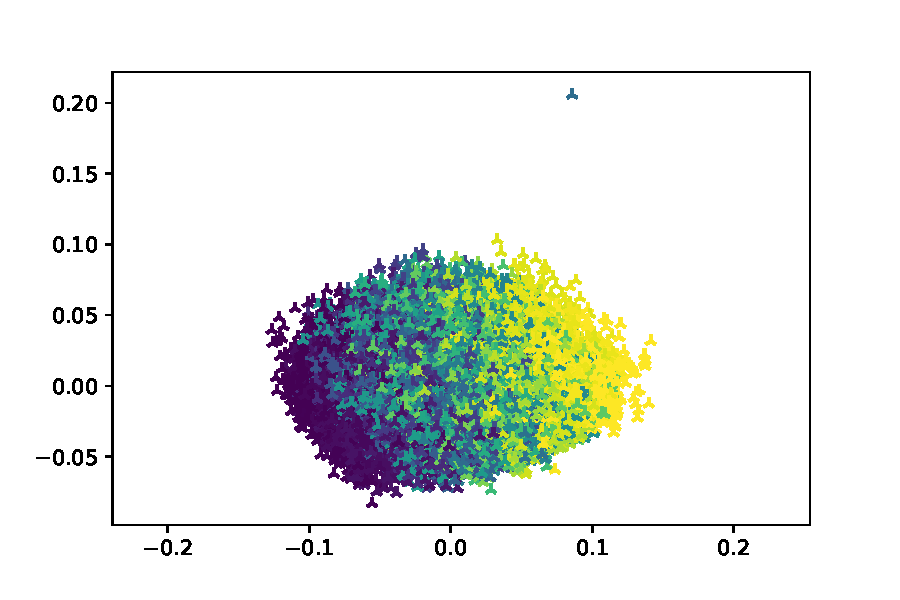
\includegraphics[width=\textwidth]{nl256_tr_instances.pdf}
\centering
\caption{PCA redukcija skupa za učenje}
\label{fig:dpa2_train_pca}
\end{subfigure}
\begin{subfigure}{.5\textwidth}
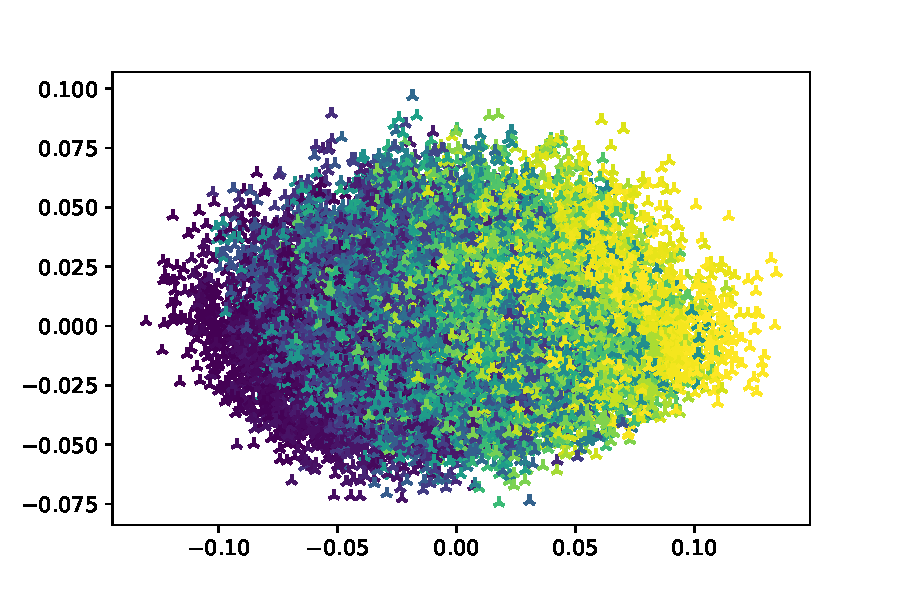
\includegraphics[width=\textwidth]{nl256_ts_instances.pdf}
\centering
\caption{PCA redukcija skupa za testiranje}
\label{fig:dpa2_test_pca}
\end{subfigure}
\begin{subfigure}{.5\textwidth}
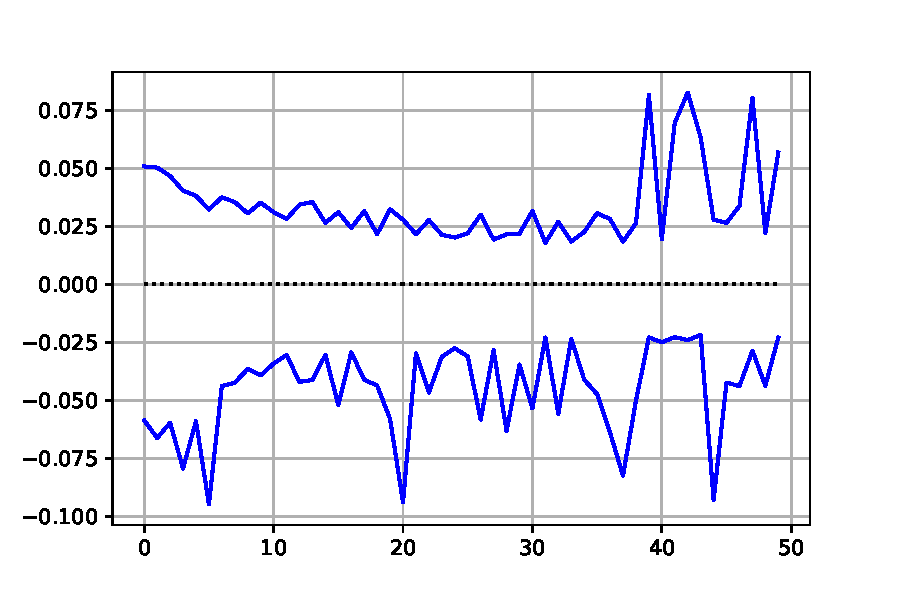
\includegraphics[width=\textwidth]{nl256_tr_inputs.pdf}
\centering
\caption{Distribucija značajki skupa za učenje}
\label{fig:dpa2_train_inputs}
\end{subfigure}
\begin{subfigure}{.5\textwidth}
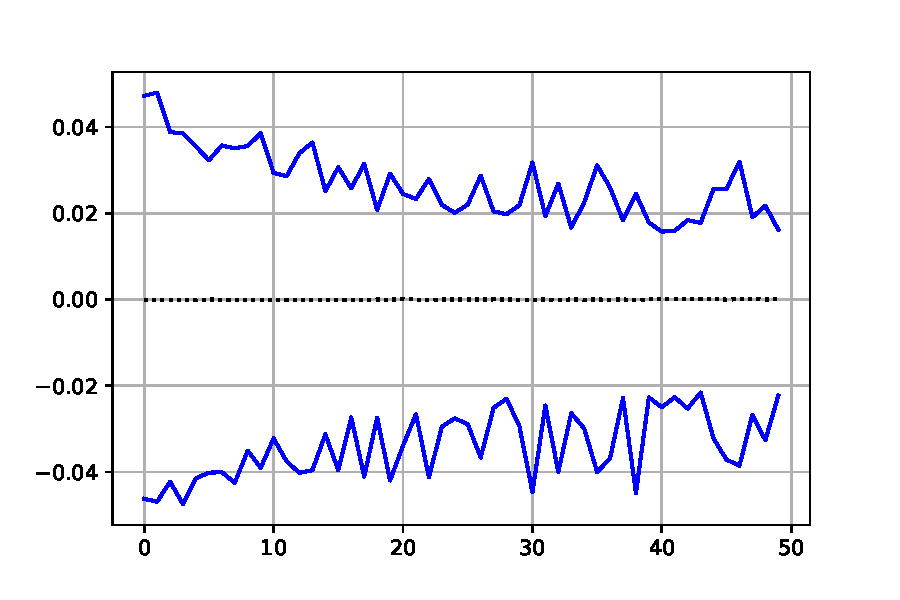
\includegraphics[width=\textwidth]{nl256_ts_inputs.pdf}
\centering
\caption{Distribucija značajki skupa za testiranje}
\label{fig:dpa2_test_inputs}
\end{subfigure}
\begin{subfigure}{.5\textwidth}
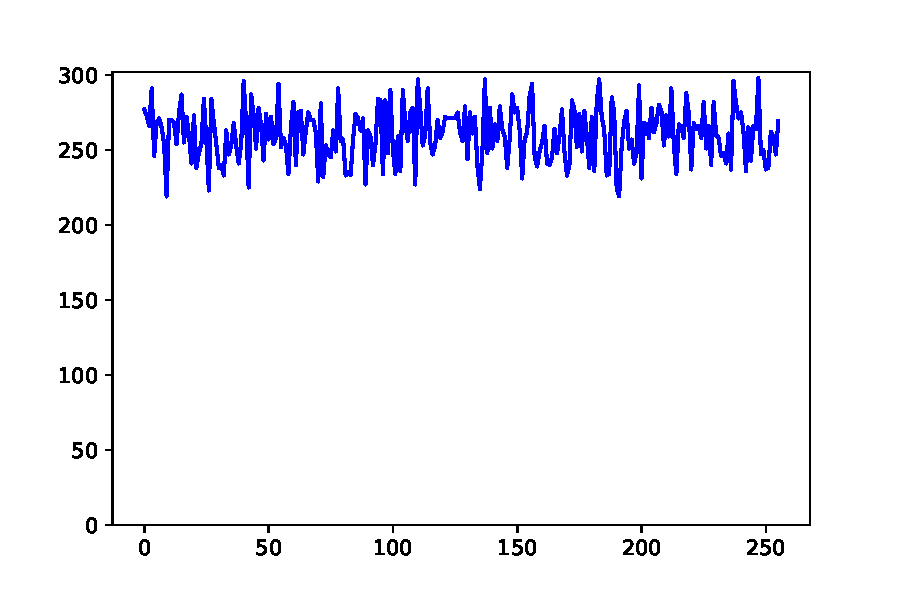
\includegraphics[width=\textwidth]{nl256_tr_outputs.pdf}
\centering
\caption{Distribucija oznaka skupa za učenje}
\label{fig:dpa2_train_outputs}
\end{subfigure}
\begin{subfigure}{.5\textwidth}
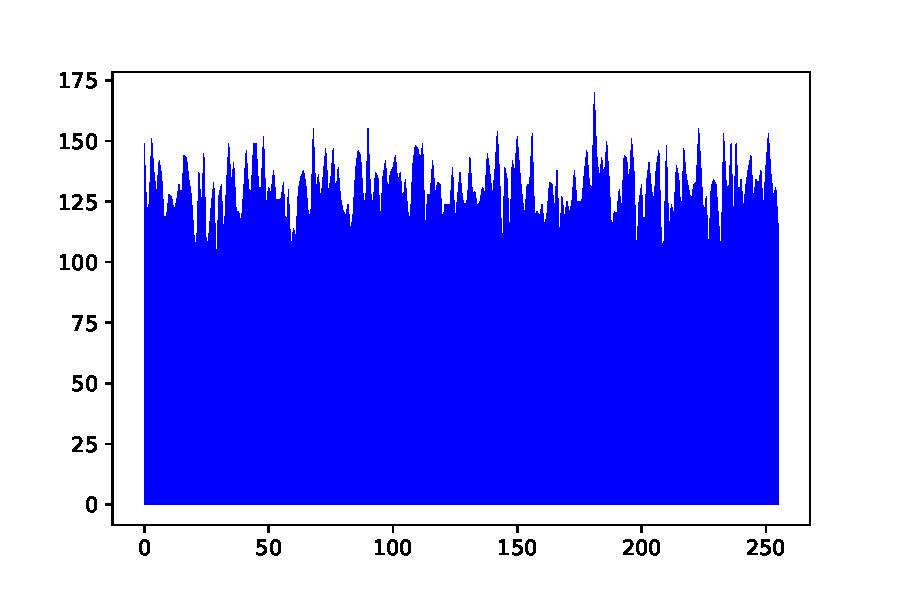
\includegraphics[width=\textwidth]{nl256_ts_outputs.pdf}
\centering
\caption{Distribucija oznaka skupa za testiranje}
\label{fig:dpa2_test_outputs}
\end{subfigure}
\caption{Statistike podskupa za učenje i testiranje skupa DPAv2}
\end{figure}

\todo{Mjere dobrote klasifikacije}

\subsection{DPAv4}
\todo{Kada je napravljen i ko ga je radilo}

\begin{figure}[H]
\begin{subfigure}{.5\textwidth}
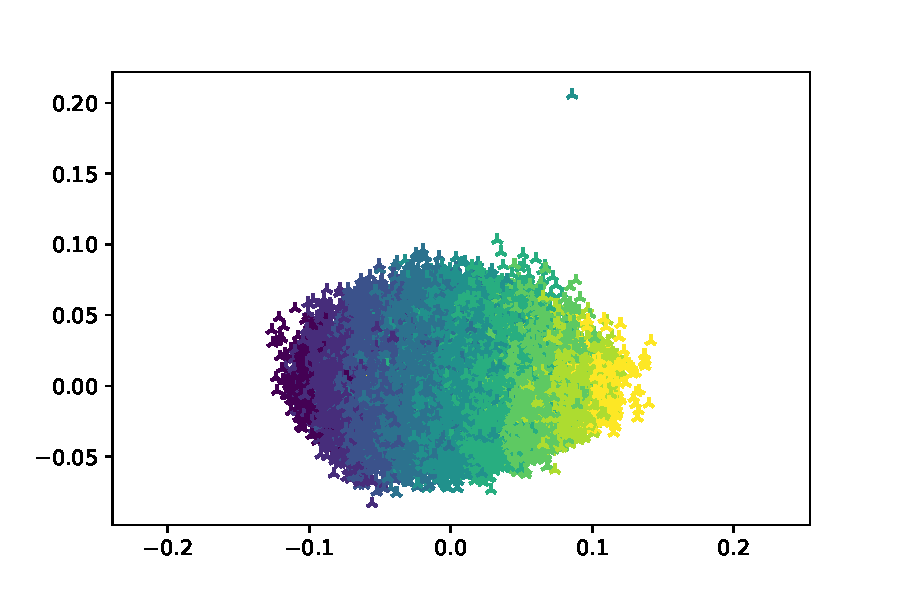
\includegraphics[width=\textwidth]{nl9_tr_instances.pdf}
\centering
\caption{PCA redukcija skupa za učenje}
\label{fig:dpa4_train_pca}
\end{subfigure}
\begin{subfigure}{.5\textwidth}
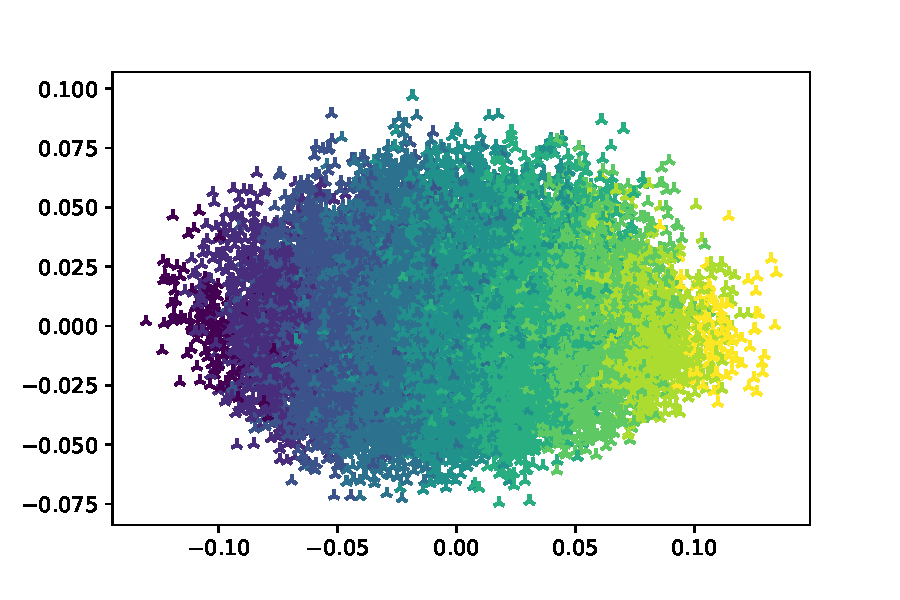
\includegraphics[width=\textwidth]{nl9_ts_instances.pdf}
\centering
\caption{PCA redukcija skupa za testiranje}
\label{fig:dpa4_test_pca}
\end{subfigure}
\begin{subfigure}{.5\textwidth}
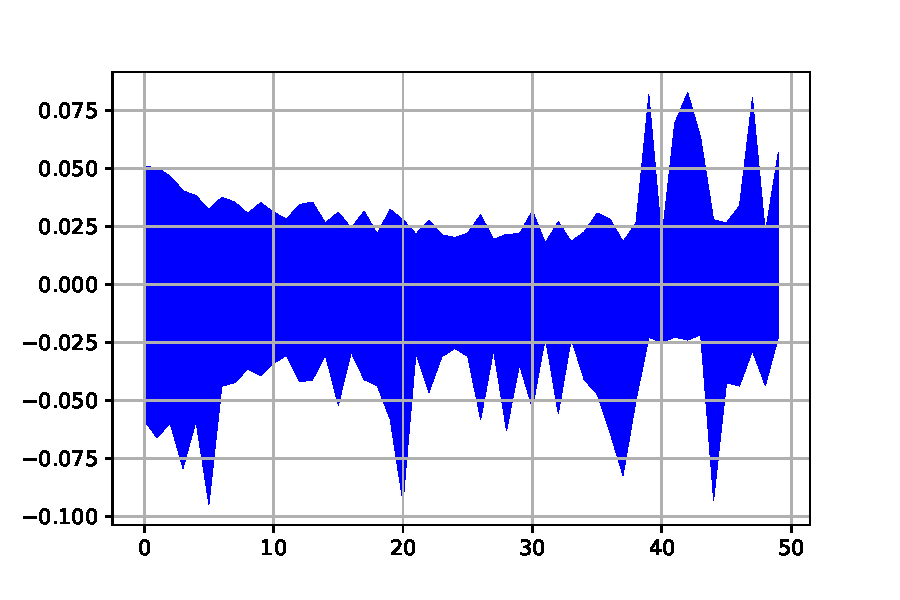
\includegraphics[width=\textwidth]{nl9_tr_inputs.pdf}
\centering
\caption{Distribucija značajki skupa za učenje}
\label{fig:dpa4_train_inputs}
\end{subfigure}
\begin{subfigure}{.5\textwidth}
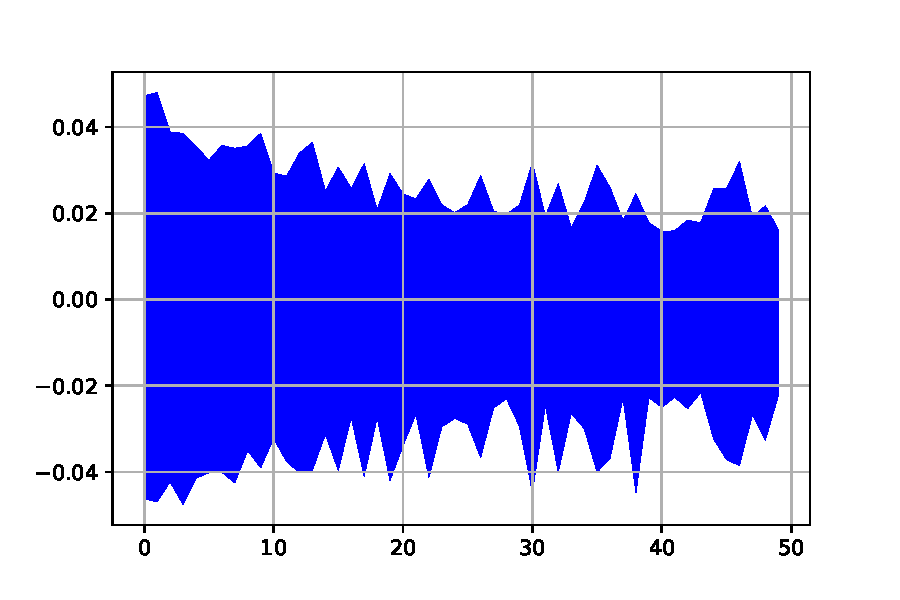
\includegraphics[width=\textwidth]{nl9_ts_inputs.pdf}
\centering
\caption{Distribucija značajki skupa za testiranje}
\label{fig:dpa4_test_inputs}
\end{subfigure}
\begin{subfigure}{.5\textwidth}
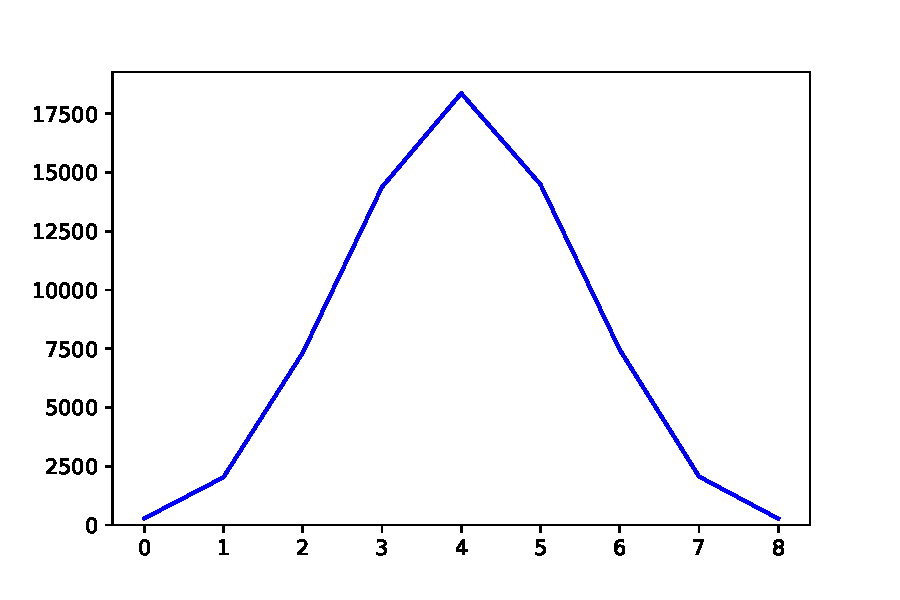
\includegraphics[width=\textwidth]{nl9_tr_outputs.pdf}
\centering
\caption{Distribucija oznaka skupa za učenje}
\label{fig:dpa4_train_outputs}
\end{subfigure}
\begin{subfigure}{.5\textwidth}
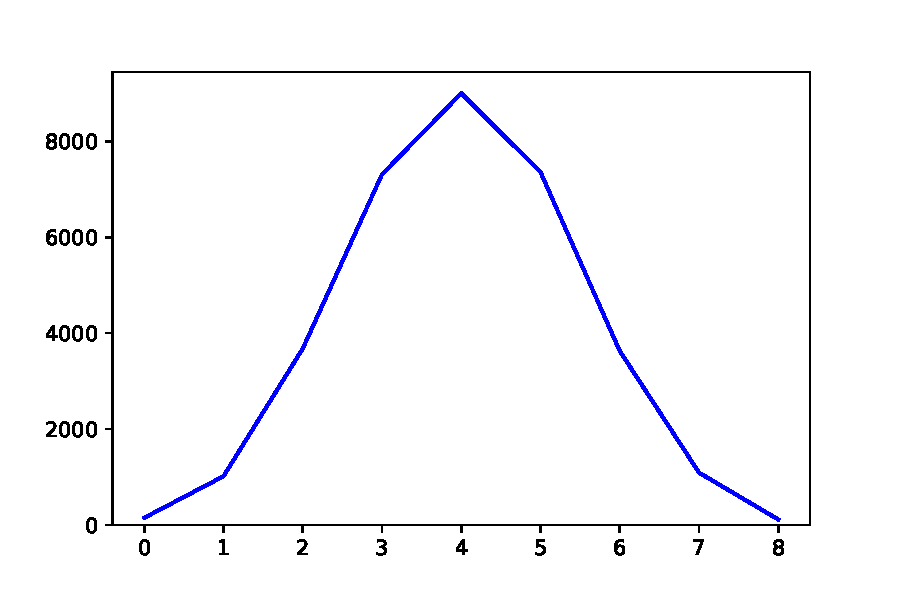
\includegraphics[width=\textwidth]{nl9_ts_outputs.pdf}
\centering
\caption{Distribucija oznaka skupa za testiranje}
\label{fig:dpa4_test_outputs}
\end{subfigure}
\caption{Statistike podskupa za učenje i testiranje skupa DPAv4}
\end{figure}

\todo{Mjere dobrote klasifikacije}

\subsection{Dosadašnji rezultati}


%--------------------------------------------------------------------------------------%
\chapter{Klasifikator temeljen na umjetnim neuronskim mrežama}

\section{Umjetne neuronske mreže}
Umjetne neuronske mreže (nadalje „neuronske mreže“) koriste se za modeliranje višedimenzijske funkcije ili distribucije kojom se aproksimira rješenje zadanog problema iz konačnog broja primjera. Vrlo su moćan alat za savladavanje teških zadataka u raznim područjima te često dostižu ljudske performanse na zadanom problemu. Danas su vrlo raširene u raznim područjima od kojih su samo neka: računalni vid \citep{alexnet,yolo}, prirodna obrada jezika \citep{word2vec,char_cnn} i podržano učenje \citep{atari,active_learn}.

\subsection{Građa}
Neuronske mreže građene su od međusobno povezanih jedinica, tzv. neurona, modeliranih prema pojednostavljenom modelu biološkog neurona. Neuron očitava ulazne značajke sustava ili izlaze drugih neurona te ažurira svoje unutarnje stanje i stvara odziv. Utjecaj ulaza na neuron vrednuje se težinama \engl{weights} koje definiraju kako se neuron ponaša u ovisnosti o pojedinim ulazima. Aktivacijski prag neurona \engl{bias} određuje jedinstvenu osjetljivost neurona na jačinu podražaja. Težine i prag neurona nazivaju se parametri neurona.

\begin{figure}[h]
\centering
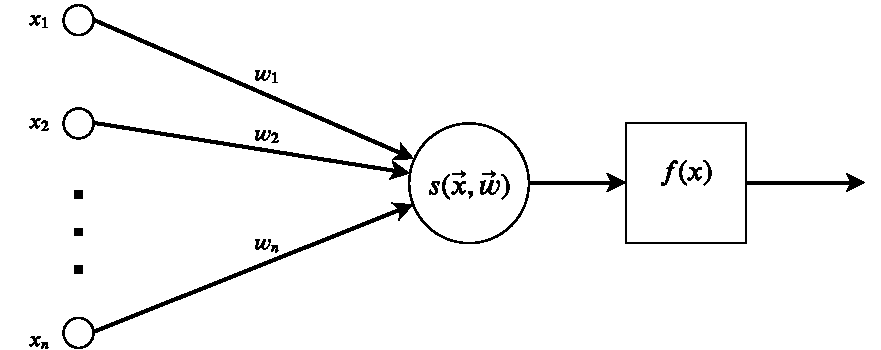
\includegraphics[scale=0.7]{Neuron.pdf}
\caption{Prikazani osnovni dijelovi neurona su težine dendrita ($w_i$), ulazna funkcija ($s(\vec{x},\vec{w})$) i aktivacijske funkcija ($f(x)$). Prag neurona nije prikazan zbog jednostavnosti dijagrama.}
\label{fig:neuron}
\end{figure}

Način na koji se iz ulaza gradi unutarnje stanje neurona opisan je ulaznom funkcijom. Pretvorba unutarnjeg stanja neurona u izlazni signal opisana je aktivacijskom funkcijom koja se detaljnije obrađuje u poglavlju \secref{sec:aktivacijske_fje}. Ulazna i aktivacijska funkcija definiraju prijenosnu funkciju koja ujedno opisuje ponašanje cijelog neurona. Pojam prijenosne funkcije je potreban jer ponekad granica između ulazne i aktivacijske funkcije nije jasna.

\begin{equation}
t(x) = (f \circ s)(x) = f(s(x))
\end{equation}

U literaturi postoje nekonzistencije oko pojma aktivacijske funkcije. U preglednim znanstvenim radovima \citep{function_survey1, function_survey2, function_survey3} pojam aktivacijske funkcije predstavlja ulaznu funkciju, što je neispravno prema brojnim današnjim radovima. Neispravno je i sa stajališta računalne neuroznanosti prema kojoj aktivacijska funkcija označava funkciju učestalosti okidanja neurona u ovisnosti o ukupnom statičkom ulazu \citep[p.~234]{neuroscience}. U starijoj literaturi pojam aktivacijske i prijenosne funkcije često se koristi ekvivalentno \citep{evolving_transfer, evo_parsimonious}. U prijedlogu standardizacije \citet{ieee_standardization} aktivacijska funkcija je definirana: \textit{„Algoritam za računanje vrijednosti aktivacije neurona kao funkcije njenog ukupnog ulaza. Ukupan ulaz je tipično težinska suma ulaza u neuron“}. S obzirom na nekonzistencije u literaturi i iz potrebe razlikovanja funkcija koje prikupljaju i odašilju signale iz neurona u ovom se radu koristi gore spomenuta nomenklatura (ulazna, aktivacijska i prijenosna funkcija).

Najpopularnije ulazne funkcije jesu afina funkcija i unakrsna korelacija.
Afina funkcija \eqref{eq:affine} je skalarni produkt vektora ulaza s vektorom težina neurona uz dodatak vrijednosti praga. Parametri neurona definiraju nagib i pomak ravnine u prostoru ulaza koja opisuje ulaz neurona. Primjenjuje se kada se ulazi u model mogu zapisati vektorom značajki čiji raspored nije bitan.
\begin{equation}
\label{eq:affine}
s(\vec{x};\mat{W},\vec{b})=\mat{W}^T \cdot \vec{x} + \vec{b}
\end{equation}

Unakrsna korelacija, za razliku od afine funkcije, koristi informaciju o susjednosti ulaznih značajki. Unakrsna korelacija vrlo je slična operatoru konvolucije te se u literaturi gotovo uvijek naziva konvolucijom. Često se koristi za ekstrakciju obrazaca u slikama \citep{alexnet}, no može se koristiti u problemima koji zahtijevaju obradu sljedova podataka. Jedan takav primjer je klasifikacija teksta u kome različit slijed riječi može prenositi različito značenje \citep{char_cnn}.

Znatno su rjeđe ulazne funkcije temeljene na udaljenosti vektora... \citep{function_survey1}
\todo{*Spomeni distance based aktivacije}

Povezivanjem neurona gradi se arhitektura mreže koja određuje kako podatci i gradijenti teku kroz mrežu, a time utječu na brzinu učenja i inferencije neuronske mreže. Najčešće se koriste slojevite unaprijedne arhitekture zbog jednostavnosti izvedbe. Unaprijedne arhitekture propuštaju podatke samo u jednom smjeru odnosno već izračunati neuroni se ne izračunavaju ponovno, što je posebno pogodno za optimizaciju širenjem unatrag\secref{sec:backprop}. Slojevite arhitekture omogućuju paralelizaciju izvođenja operacija na grafičkim karticama što značajno ubrzava postupke učenja i inferencije. Pri definiciji slojevite arhitekture najčešće je dovoljno navesti samo redoslijed slojeva, no ponekad je potrebno definirati i način povezivanja slojeva npr. pri uporabi preskočnih veza \citep{highwaynet, resnet, densenet}. Prvi sloj služi za postavljanje ulaza mreže i naziva se ulaznim slojem mreže. Posljednji sloj mreže služi nam za ekstrakciju izlaza te mjerenje kakvoće mreže i naziva se izlaznim slojem mreže. Svi slojevi između ulaznog i izlaznog sloja nazivaju se skrivenim slojevima.

Potpuno povezana arhitektura je najjednostavnija arhitektura. Svaki neuron u potpuno povezanom sloju aktivira se pomoću svih izlaza iz prethodnog sloja. Za naučeni potpuno povezani sloj kaže se da vrši ekstrakciju značajki iz svojih ulaza. Geometrijski gledano, svaki neuron vrši nelinearno mapiranje značajki iz dimenzije prethodnog sloja u novu dimenziju s ciljem modeliranja boljih značajki.

\subsection{Optimizacija umjetne neuronske mreže}
Optimizacijom parametara neuronska mreža prilagođava se danom zadatku, odnosno kaže se da mreža 'uči'. Optimizacija parametara najčešće se izvodi gradijentnim spustom, uz pretpostavku derivabilnosti svih komponenata neuronske mreže. Kada ta pretpostavka ne vrijedi koriste se algoritmi kombinatorne optimizacije poput algoritma roja čestica koji se spominje u \citet{skripta_nenr}. U ovom radu neuronske mreže optimiraju se gradijentnim spustom.

\subsubsection{Gradijentni spust}
\label{sec:gradijentni_spust}

\todoimg{gradijentni spust unimodalna vs višemodalna (gdje preskoči brdo i uleti u bolji optimum)}
\label{fig:gradientni_spust}

Gradijentni spust je algoritam pronalaska minimuma funkcije vođen gradijentom te funkcije. Za zadanu početnu točku iterativno se pomiče u smjeru suprotnom od gradijenta funkcije u toj točki dok ne zadovolji neki od uvjeta zaustavljanja. Na strmim funkcijama gradijent je često prevelik i može izazvati oscilaciju ili divergenciju \figref{fig:oscilira_divergira}. Stoga se gradijent pri pomaku skalira koeficijentom pomaka $\mu$. Dobro odabran koeficijent pomaka može osigurati bržu konvergenciju, a kod višemodalnih funkcija i pronalazak boljeg optimuma \figref{fig:gradientni_spust}.

Početna točka utječe na ishod algoritma. Kod višemodalnih funkcija s optimumima različitih kvaliteta, početna točka može definirati u koji će lokalni optimum algoritam konvergirati \figref{fig:pocetna_tocka}.
\newline
\newline
\begin{algorithm}[H]
\DontPrintSemicolon
\KwIn{funkcija $f(\vec{x})$}
\KwIn{početna točka $\vec{x}_0$}
\KwIn{koeficijent pomaka $\eta$}
\KwIn{broj iteracija $n$}
\For{n iteracija}{
$\vec{g}_i \gets \vec{\nabla}_{\vec{x}} f(\vec{x}_i)$ \;
$\vec{x}_{i+1} \gets \vec{x}_i - \eta \cdot \vec{g}_i$
}
\KwResult{pronađena optimalna točka $\vec{x}_i$}
\;
\caption{Gradijentni spust}
\label{alg:grad_spust}
\end{algorithm}

\todoimg{gradijentni spust stope spuštanja (velka, mala, taman)}
\label{fig:oscilira_divergira}

Broj iteracija definira broj pomaka od početne točke, što definira i trajanje algoritma. Generalno želi se skratiti vrijeme pretraživanja te povećati koeficijent spusta kako bi se koristilo manje pomaka. No u praksi se najčešće nailazi na višemodalne funkcije sa strmim regijama koje izazivaju oscilacije i mogu izazvati divergenciju. Stoga se češće koriste manji pomaci kroz više iteracija. Dodatno se mogu dodati modifikacije gradijenta koje nude ograničavaju veličinu gradijenta (odsijecanje gradijenta i sl.).

\todoimg{gradijentni spust s početnim točkama (jedna ode u lok, jedna ode u glob, jedna zapne desno na platou)}
\label{fig:pocetna_tocka}

Problem se javlja ako algoritam odluta u visoravan na kojoj su gradijenti vrlo mali, a sama regija je s obzirom na pomake ogromna \figref{fig:pocetna_tocka}. Kad gradijent postane neupotrebljivo malen kaže se da je \textit{nestao}. U takvim slučajevima pomaže dodavanje momenta koji se akumulira kroz više iteracija i dodaje vektoru gradijenta. Kad algoritam naiđe na regiju s vrlo malim gradijentima, moment pokušava izvući algoritam iz visoravni pomičući ga u smjeru koji je akumuliran. Kako moment ne bi izvukao algoritam iz optimuma, dodaje mu se koeficijent \textit{zaboravljanja} kojim se stari vektor momenta djelomično zaboravlja u korist novog vektora pomaka (jednadžba \ref{eq:moment_update}). Moment može pomoći i pri zaobilaženju lokalnih optimuma \figref{fig:pocetna_tocka}.

\begin{equation}
\label{eq:moment_update}
\begin{split}
\vec{v} &\gets \alpha \cdot \vec{v} - \eta \cdot \vec{g} \\
\vec{x} &\gets \vec{x} + \vec{v}
\end{split}
\end{equation}

\todoimg{moment prije i na visoravni, moment za savladavanje brda}
\label{fig:visoravan}

Algoritam je primjenjiv na funkcije proizvoljne dimenzionalnosti uz pretpostavku derivabilnosti u svakoj točki. Za proizvoljnu realnu funkciju, uz dobro odabrane hiperparametre, algoritam će konvergirati u jedan od lokalnih optimuma, no algoritam generalno nema garanciju konvergencije u globalni optimum. Garanciju pronalaska globalnog optimuma nudi jedino za trivijalne unimodalne funkcije uz odgovarajuće hiperparametre algoritma \figref{fig:gradientni_spust}.

Problem odabira hiperparametara proizlazi iz činjenice da u generalno praksi funkcija koja se minimizira nije definirana (već samo skup primjera te funkcije) te se ne može jasno vizualizirati postupak pretrage. Čak i da je definirana funkcija najčešće nije poznata vrijednost globalnog optimuma, a pohlepna pretraga je netraktabilna. Unatoč tome, gradijentni spust efikasno i učinkovito pronalazi optimume koji su dovoljno dobri za većinu praktičnih primjena \citep{yolo}.

\subsubsection{Funkcija gubitka}
Pri učenju umjetnih neuronskih mreža potrebno je definirati funkciju gubitka. Funkcija gubitka, za dani ulaz, uspoređuje predikciju mreže sa željenim vrijednostima te dodjeljuje iznos pogreške (realan broj). Potrebno je pažljivo odabrati funkciju gubitka jer utječe na učenje svakog parametra \secref{sec:backprop} te definira što je ishod učenja. 

Najčešće nije poznata definicija funkcije gubitka na čitavoj promatranoj domeni već su poznati samo primjeri te funkcije u podatcima koji su izmjereni i koji se smatraju reprezentativnim. Ovdje se pretpostavlja da će neuronska mreža ostvariti svojstvo generalizacije, koje je detaljnije objašnjeno u poglavlju \ref{sec:svojstva}. Stoga se u narednim formulama koristi notacija sumiranja.

Funkcija gubitka često je usko vezana uz vrstu problema koji se rješava (klasifikacija, regresija i ostali), način učenja (nadzirano, polu-nadzirano, nenadzirano, podržano) i aktivacijsku funkciju posljednjeg sloja neuronske mreže. U ovom radu vrši se klasifikacija nadziranim učenjem, no u nastavku se navodi i primjer funkcije gubitka za regresiju. Funkciju gubitka definira se kao inverz funkcije izglednosti da neuronska mreža modelira funkciju predstavljenu primjerima podatkovnog skupa. Funkcija gubitka se minimizira pa je definirana \textbf{negativnim logaritmom izglednosti} \eqref{eq:negloglikelyhood}. Logaritam je uveden zbog pojednostavljivanja distribucija koje sadrže eksponente.

\begin{equation}
\label{eq:negloglikelyhood}
L(\theta \probsep x,y) = -\log\ p(f(X;\theta)=y \probsep X=x)
\end{equation}

Zbog jednostavnosti zapisa, funkcija modela zapisuje se skraćeno kao aproksimacija odnosno predikcija funkcije izlaza podatkovnog skupa te se ovisnost o ulazima podrazumijeva.
\begin{equation}
\hat{y} = f(x; \theta)
\end{equation}

S obzirom da se želi procijeniti kvaliteta modela na čitavom podatkovnom skupu važno je očekivanje funkcije gubitka \eqref{eq:negloglikelyhood_expect}.
\begin{equation}
\label{eq:negloglikelyhood_expect}
\begin{split}
L(\theta \probsep \dataset) &= \expect_{(x,y) \sim p_\dataset}[L(\theta \probsep x,y)] \\
&= -\frac{1}{|\dataset|} \sum_{(x,y)\in\dataset} \log\ p(\hat{y}=y \probsep x)
\end{split}
\end{equation}

\textbf{U problemima regresije}, pretpostavlja se da izlazi mreže prate Gaussovu distribuciju s jediničnom kovarijacijskom matricom. Njenim uvrštavanjem u negativnu log. izglednost \eqref{eq:negloglikelyhood} dobiva se funkcija kvadratnog gubitka koja računa odstupanje izlaza neuronske mreže od željenih vrijednosti. Uz ovaj gubitak najčešće se koristi funkcija identiteta u izlaznom sloju.
\begin{align}
\label{eq:normal_dist}
\begin{split}
p(\hat{y}=y \probsep x) &= \normal(y \probsep \mu=\hat{y}, \mat{\Sigma}=\mat{I}) \\
&= \frac{1}{\sqrt{2\pi}\Sigma^{^1/_2}} \exp(-(y-\hat{y})^T\Sigma^{^1/_2}(y-\hat{y}))
\end{split}
\end{align}

Uvrštavanjem u \eqref{eq:negloglikelyhood} dobiva se kvadratni gubitak:

\begin{align}
\label{eq:loss_regression}
L(\theta \probsep x,y) &= - \log \Big[ \frac{1}{\sqrt{2\pi}\Sigma^{^1/_2}} \Big] - \log \Big[ \exp(-(y-\hat{y})^T\Sigma^{^1/_2}(y-\hat{y})) \Big] \nonumber \\
&= -\log c - (y-\hat{y})^T\Sigma^{^1/_2}(y-\hat{y}) \nonumber \\
&= \left|\footnotesize 
\begin{array}[c]{l} 
	c = konst. \\ 
	\Sigma = I 
\end{array}
\right| \nonumber \\
&= (y-\hat{y})^T(y-\hat{y}) = \sum_i (y_i - \hat{y}_i)^2
\end{align}

\textbf{U problemima klasifikacije}, pretpostavlja se da su izlazi mreže međusobno isključive slučajne varijable te stoga prate generaliziranu Bernoullijevu distribuciju (kategoričku distribuciju).
\begin{equation}
p(\hat{y}=y \probsep x) = \hat{y}_1^{y_1} \cdot \hat{y}_2^{y_2} \cdots \hat{y}_c^{y_c} 
= \prod_{i=1}^C \hat{y}_i^{y_i}, \quad \sum_i \hat{y}_i = 1
\end{equation}

Uvrštavanjem u \ref{eq:negloglikelyhood} dobiva se kategorički gubitak:
\begin{align}
\label{eq:loss_classification}
L(\theta \probsep x,y) &= - \log \Big[ \prod_{i=1}^C \hat{y}_i^{y_i} \Big] = - \sum_{i=1}^C y_i \log (\hat{y}_i)
\end{align}

\subsubsection{Optimizacija širenjem unatrag}
\label{sec:backprop}
Funkcija gubitka opisuje pogrešku čitave mreže te ovisi o svakom prilagodljivom parametru mreže. Takva formulacija problema omogućuje nam da svaki parametar mreže ugađa se gradijentnim spustom. Dakle, za parametriziranu funkciju $f(x;\theta)$ traže se parametri $\theta^*$ za koje je gubitak najmanji na podatkovnom skupu.
\begin{equation}
\theta^* = argmin_\theta\ L(\theta \probsep \dataset), \quad \forall (x,y) \in \dataset
\end{equation}

Optimiranje gradijentnim spustom zahtjeva derivabilnost funkcije koja se optimizira po ulazima, što izrazi \eqref{eq:loss_regression} i \eqref{eq:loss_classification} zadovoljavaju. Pri tome koristi se pravilo ulančavanja parcijalne derivacije kompozicije funkcija.
\begin{equation}
\label{eq:partial_rule}
\dfrac{}{x} f(g(x)) = \pfrac{f(g(x))}{g(x)} \cdot \pfrac{g(x)}{x}
\end{equation}

Derivacijom funkcije gubitka za regresiju \eqref{eq:loss_regression} po ulazima, uz pretpostavku derivabilnosti čitave neuronske mreže po ulazima, dobiva se sljedeći izraz:
\begin{align}
\dfrac{L(\theta \probsep x,y)}{x} &= \dfrac{}{x}\sum_i(y_i - \hat{y}_i(x))^2 \nonumber \\
&= 2 \cdot \sum_i (y_i - \hat{y}_i(x)) \cdot \dfrac{\hat{y}_i(x)}{x}
\end{align}

Derivacija funkcije gubitka za klasifikaciju može se drastično pojednostaviti ako se za funkciju izlaznog sloja mreže odabere funkcija \textit{softmax} \eqref{eq:softmax_for_loss}, a izlazi se kodiraju \textit{one-hot} oznakama \eqref{eq:onehot}. Ulaz u funkciju softmax su aktivacije neurona izlaznog sloja koje su ovdje označene vektorom $\vec{s}(x)$.
\begin{equation}
\label{eq:softmax_for_loss}
\hat{y}(\vec{x}) = \text{softmax}(\vec{s}(x)) = \frac{\exp(\vec{s}(x))}{\sum_{i=1}^{C} exp(s_i(x))}
%%% \quad \equiv \quad p(y_i \probsep x) = \frac{p(x|y_i)p(y_i)}{\sum_jp(x|y_j)p(y_j)}
\end{equation}

\begin{equation}
\label{eq:onehot}
\vec{y}=[y_1, y_2, \cdots, y_C], \quad y_i \in \{0,1\}, \quad \sum_{i=1}^C y_i = 1
\end{equation}

Uvrštavanjem u \eqref{eq:loss_classification} dobivamo:

\begin{align}
\label{eq:loss_classification_softmax}
L(\theta \probsep x,y) &= - \sum_{i=1}^C y_i \log \frac{\exp(s_i(x))}{\sum_{j=1}^{C} exp(s_j(x))} \nonumber \\
&= - \sum_{i=1}^C \bigg[ y_i \cdot s_i(x) - y_i \log\big(\sum_{j=1}^{C} exp(s_j(x))\big) \bigg] \nonumber \\
&= - \sum_{i=1}^C \big[ y_i \cdot s_i(x) \big] + \log\big[\sum_{j=1}^{C} exp(s_j(x))\big] \cdot \sum_{i=1}^C y_i \nonumber \\
&= \log\big[\sum_{j=1}^{C} exp(s_j(x))\big] - \sum_{i=1}^C \big[ y_i \cdot s_i(x) \big]
\end{align}

Derivacijom \eqref{eq:loss_classification_softmax} po ulazima, koristeći pravilo \eqref{eq:partial_rule} dobivamo:
\begin{align}
\dfrac{L(\theta \probsep x,y)}{x} &= \dfrac{L(\theta \probsep x,y)}{\vec{s}(x)} \cdot \dfrac{\vec{s}(x)}{x} \nonumber \\
&= \bigg[ \vec{s}(x) - y \bigg] \cdot \dfrac{s(x)}{x}
\end{align}

S obzirom da se mreža sastoji od ulančanih nelinearnih neurona s parametrima, gradijent gubitka mora se proslijediti sekvencijalno širenjem unazad (prema ulazima u mrežu). Pojedini neuron može se smatrati parametriziranom funkcijom koju je moguće prikazati grafom. Ulazni gradijent prolaskom kroz neuron širi se na ostale elemente i na ulaze neurona koji vode do prethodnih neurona. Dodatno, gradijent se širi u suprotnom smjeru od toka podataka. Iz toga proizlazi naziv \textit{širenjem unazad} \engl{backpropagation}.

Želi li se mrežu učiti gradijentnim spustom, svaki parametar mreže treba imati pristup gradijentu funkcije gubitka. S obzirom da je neuron parametrizirana funkcija, pomoću koje se ulančavanjem gradi mreža, dovoljno je pokazati da pojedini neuron osigurava svojim parametrima pristup gradijentu te da gradijent šalje svojim prethodnicima s kojima je povezan. Da je to ostvarivo dokazuju izrazi:
\begin{align}
\begin{split}
\pfrac{L(x,y;\theta)}{s(x;w)} &= \pfrac{L(x,y;\theta)}{o(x;w)} \cdot \pfrac{o(x;w)}{s(x;w)} \\
&= \pfrac{L(x,y;\theta)}{o(x;w)} \cdot f'(x)
\end{split}
\end{align}

\begin{align}
\begin{split}
\pfrac{L(x,y;\theta)}{x_i} &= \pfrac{L(x,y;\theta)}{s(x;w)} \cdot \pfrac{s(x;w)}{x_i} \\
&= \pfrac{L(x,y;\theta)}{o(x;w)} \cdot f'(x) \cdot w_i
\end{split}
\end{align}

\begin{align} \label{eq:w_update}
\begin{split}
\pfrac{L(x,y;\theta)}{w_i} &= \pfrac{L(x,y;\theta)}{s(x;w)} \cdot \pfrac{s(x;w)}{w_i} \\
&= \pfrac{L(x,y;\theta)}{o(x;w)} \cdot f'(x) \cdot x_i
\end{split}
\end{align}

\begin{align}
\begin{split}
\pfrac{L(x,y;\theta)}{w_0} &= \pfrac{L(x,y;\theta)}{s(x;w)} \cdot \pfrac{s(x;w)}{w_0} \\
&= \pfrac{L(x,y;\theta)}{o(x;w)} \cdot f'(x) \cdot 1
\end{split}
\end{align}

\subsubsection{Stohastički gradijentni spust}
U prošlom poglavlju korištena je funkcija gubitka na jednom podatkovnom paru, no želi se minimizirati očekivanje funkcije gubitka \eqref{eq:negloglikelyhood_expect} na cijelom podatkovnom skupu jer se želi izgraditi model da aproksimira čitavu uzorkovanu funkciju što bolje. Nažalost, podatkovni skupovi poput spomenutog u poglavlju \ref{sec:dpa_datasets} vrlo su veliki i nije ih praktično koristiti pri optimizaciji gradijentom jer bi se čitavi morali držati u brzoj memoriji. Ovo predstavlja velik problem pri računanju s grafičkim karticama. Očekivanje gubitka služi nam za procjenu smjera i veličine gradijenta. Ako se gradijent procjenjuje na čitavom podatkovnom skupu on će nas dovesti do prvog optimuma koji najčešće nije dobar, odnosno snažno ovisi o odabiru početne točke. 

S druge strane, ako se gradijent računa na pojedinom podatkovnom paru kao u \eqref{eq:loss_classification} ostvareno je stohastičko kretanje jer će svaki primjer usmjeriti gradijent u drugom smjeru. Posljedica toga je dulje vrijeme pretrage, no veća otpornost na loše lokalne optimume. Iako će algoritam generalno konvergirati, postupak je zahtjevan jer za svaki primjer podatkovnog skupa treba provesti korak algoritma. Ovaj problem također ograničava svojstvo ubrzanja grafičkim karticama koje nude masivnu paralelizaciju operacija nad podatcima.

Iz navedenih razloga želi se vršiti procjena gradijenta na "nekoliko" primjera. Podskup takvih primjera naziva se \textbf{mini-grupa} \engl{mini-batch}. Najčešće se uzima najveći broj primjera koji grafička kartica može efikasno obraditi i koji je potencija broja 2. Mini-grupe i dalje zadržavaju stohastičnost kretanja gradijenta (posebice ako je veličina manja od broja klasa), ali procjenjuju bolje od potpuno stohastičnog te brže konvergiraju. Sada formula \eqref{eq:negloglikelyhood_expect_minibatch} poprima oblik koji odgovara očekivanju pojedine mini-grupe $\minibatch_i$.
\begin{equation}
\label{eq:negloglikelyhood_expect_minibatch}
\begin{split}
L(\theta \probsep \dataset) &= \expect_{(x,y) \sim p_{\minibatch_i}}[L(\theta \probsep x,y)] \\
&= -\frac{1}{|\minibatch_i|} \sum_{(x,y)\in\minibatch_i} \log\ p(\hat{y}=y \probsep x)
\end{split}
\end{equation}

Mini-grupe se najčešće definiraju prije početka učenja nasumičnim rasporedom. To je najjednostavniji i najbrži pristup, no definiranjem fiksnih mini-grupa unosi induktivnu pristranost jer nije moguće znati je li odabrani raspored idealan za model koji se evaluira. Pristranost se može ublažiti miješanjem podatkovnog skupa između epoha, no skupocjenost te operacije ograničava njeno korištenje u praksi. Također, problem mogu stvoriti mini-grupe pristrane jednoj ili više dominantnih (većinskih) klasa koje će snažno usmjeravati gradijent prema tim klasama i zanemarivati ostale. Taj problem je posebno izražen u nebalansiranim podatkovnim skupovima, a može se zaobići tehnikom težinskog uzorkovanja s ponavljanjem gdje je vjerojatnost odabira primjera obrnuto proporcionalna dominantnosti (brojnosti) njegove klase. Treba paziti da se provede dovoljan broj uzorkovanja tako da je model učen na svakom primjeru podatkovnog skupa.
\newline
\newline
\begin{algorithm}[H]
\DontPrintSemicolon
\KwIn{funkcija $f(\vec{x})$}
\KwIn{početni parametar $\vec{\theta}_0$}
\KwIn{stopa učenja $\eta$}
\KwIn{kriterij zaustavljanja $k$}
\While{kriterij $k$ nije zadovoljen}{
	\For{$\minibatch_i \in \dataset$}{
		$\vec{g}_i \gets \frac{1}{|\minibatch|} \sum_{(\vec{x},\vec{y})\in\minibatch} \vec{\nabla}_{\theta} L(\theta \probsep \vec{x},\vec{y})$ \;
		$\vec{\theta}_{i+1} \gets \vec{\theta}_i - \eta \cdot \vec{g_i}$
	}
}
\KwResult{pronađeni optimalni parametar $\vec{\theta}^*$}
\;
\caption{Stohastički gradijentni spust}
\label{alg:sgd}
\end{algorithm}

\subsubsection{Optimizator}
Optimizator brine o pomaku odnosno ažuriranju parametara modela pri gradijentnom spustu. Dosad su objašnjena dva pristupa: klasični s koeficijentom pomaka (algoritam \ref{alg:grad_spust}) i s dodatkom momenta \eqref{eq:moment_update}.

Optimizator Adam \engl{adaptive moments} dodatno prati povijest momenta drugog reda kojom prilagođava stopu učenja kako bi smanjio razlike između parametara koji su povijesno dobivali velike ili male gradijente, čime se izglađuje prostor parametara. Povijest drugog momenta prate AdaGrad i RMSProp, no Adam dodatno prati povijest prvog momenta i uključuje centriranje momenata. Adam se pokazao vrlo robusnim optimizatorom i vrlo često se koristi za optimizaciju dubokih neuronskih mreža. \citep{goodfellowbook}

\subsubsection{Promjenjiva stopa učenja}
Tijekom optimizacije gradijentnim spustom uz fiksnu stupu učenja optimizacija će početi oscilirati oko iste vrijednosti, odnosno srednja vrijednost gubitka je konvergirala. Oscilacija se javlja jer je stopa učenja suviše velika za regije u koje vode različiti gradijenti mini-grupa. U takvim situacijama je potrebno smanjiti stopu učenja, no problem je detekcija takvih situacija. Optimizator Adam prilagođava gradijente skaliranjem, odnosno istovjetno možemo reći da prilagođava stopu učenja \citep{goodfellowbook}. Unatoč tome, ponekad je potrebno koristiti dodatne mehanizme smanjivanja stope učenja.

%Jedan način smanjivanja stope je zadavanje ključnih iteracija u kojima se prestaje koristiti stara stopa i koristi se nova. Moguće je zadati stope za svaku od zadanih ključnih iteracija %\citep{onaj rad} ili zadati početnu stopu koja se u ključnoj iteraciji pomnoži konstantom manjom od 1. Pri ovom pristupu problem je odrediti optimalne ključne iteracije ili početnu iteraciju i konstantu.
%\todo{fali tekst (nađi onaj rad)}

%Ključnim iteracijama mogu se proglasiti one u kojima je detektirana konvergencija ili divergencija. Taj pristup omogućava nastavak pretrage, no problem je kako sa sigurnošću detektirati konvergenciju ili divergenciju. Tipično učenje mreže nije monotono, tj. gubitak mreže može na neko vrijeme rasti prije no što nastavi padati, što odgovara ponašanju u lokalnom optimumu. U tom slučaju smanjivanje stope učenja je nepoželjno.

Pristup koji se koristi u ovom radu je zadanu početnu stopu u svakoj iteraciji pomnožiti s konstantom manjom od 1, odnosno stopa se konstantno smanjuje. Korištenje stohastičkog gradijentnog spusta postupak vodi pretragu na sve finije regije. Postupak je sličan postupku simuliranog kaljenja gdje se smanjivanjem temperature sustava smanjuje njegova stohastičnost i postupak konvergira u sve finije regije rješenja. Iako bi u teoriji Adam trebao biti dovoljan, preliminarni eksperimenti pokazuju da dodani mehanizam pomaže učenju mreže.

\subsubsection{Inicijalizacija parametara}
Inicijalizacija parametara mreže odgovara odabiru početne točke pri gradijentnom spustu. Dobrom inicijalizacijom može se osigurati pronalazak boljeg optimuma te u kritičnim slučajevima i osigurati konvergencija mreže. S obzirom da neuronske mreže posjeduju jasnu strukturu (što je posebno izraženo u slojevitim arhitekturama) inicijalizacija ima dodatne utjecaje. U potpuno povezanim slojevima želi se postići da svaki neuron vrši ekstrakciju značajki. Pri tome, u efikasnom sloju svaki će neuron stvoriti svoju značajku. Ako je više neurona inicijalizirano dovoljno slično, ti neuroni će naučiti izvlačiti iste značajke. Kaže se da je došlo do \textbf{koadaptacije neurona}.

Inicijalizacija slojevitim nenadziranim učenjem ograničenog Boltzmann-ovog stroja \engl{restricted Boltzmann machine} pokazuje se dobrom \citep{relu6}. Postupak nenadzirano trenira stohastičku mrežu sloj po sloj na ulaznim značajkama kako bi slojevi ostvarili dobru ekstrakciju viših značajki. Nakon treniranja, mreži se dodaje izlazni klasifikacijski sloj i mreža se nadzirano ugađa na skupu za učenje. Iako je ostvarena inicijalizacija vrlo dobra, postupak je vremenski zahtjevan. Uvođenjem 

%\todo{postoji i init. autoenkoderom, ali u kontekstu evolucije je preskupa}

U ovom radu koristi se Xavier inicijalizacija koja parametre uzorkuje iz centrirane normalne distribucije s varijancom koja ovisi o broju ulaznih i izlaznih neurona. \citep{xavier}
\begin{equation}
W_{i,j} \sim \normal(0, \frac{2}{n_{ulaza}+n_{izlaza}})
\end{equation}

\subsubsection{Normalizacija značajki}
Podatci najčešće nisu uzorkovani iz normalne distribucije. To stvara problem jer prisiljava mrežu da uči srednju vrijednost i varijancu što usporava učenje i stvara numeričke probleme. Stoga je korisno prije korištenja svesti značajke na normalnu distribuciju sa sredinom $0$ i varijancom $1$. To se izvodi računanjem koeficijenata distribucije te oduzimanjem sredine i dijeljenjem s varijancom.

Koeficijenti se računaju iz značajki podatkovnog skupa za učenje. Koeficijent varijance ovisi o koeficijentu sredine pa se njihovo računanje ne može paralelizirati, no to ne predstavlja velik problem s obzirom da se računaju samo jednim prolazom kroz skup.
\begin{equation}
\vec{\mu} = \frac{1}{N} \sum_{\vec{x}\in \dataset} \vec{x}
\end{equation}
\begin{equation}
\vec{\sigma^2} = \frac{1}{N-1} \sum_{\vec{x}\in \dataset} (\vec{x}-\vec{\mu})^2
\end{equation}

Prije no što se značajke predaju modelu normaliziraju se formulom \eqref{eq:feat_norm}.
\begin{equation}
\label{eq:feat_norm}
\vec{z} = \frac{\vec{x} - \vec{\mu}}{\vec{\sigma^2}}
\end{equation}

Koeficijenti normalizacije računaju se isključivo na skupu za učenje, a normalizacija se mora primijeniti prilikom inferencije odnosno na skupu za testiranje.

\subsubsection{Normalizacija nad grupom}
\engl{batch normalization}

Pri optimizaciji neuronskih mreža u jednoj iteraciji se optimiziraju svi parametri. Problem pri tome je što predikcija optimizatora za parametre jednog sloja pretpostavlja da će ostali slojevi ostati netaknuti. To uzrokuje promjenu srednje vrijednosti i varijance odziva koja se akumulira prolaskom kroz mrežu. Iz tog razloga koristi se normalizacija grupom koja standardizira odzive neurona po svakoj mini-grupi. Kako to može smanjiti ekspresivnost neurona, koristi se naknadna afina transformacija s učećim parametrima.
\begin{align}
\mu &= \frac{1}{N} \sum_{i=1}^N h_i \qquad
\sigma^2 = \frac{1}{N} \sum_{i=1}^N (h_i-\mu)^2 \\
\hat{h}_i &= \frac{h_i - \mu}{\sqrt{\sigma^2 + \epsilon}} \qquad
y_i = \gamma \cdot h_i + \beta
\end{align}

\subsection{Regularizacija}
\label{sec:regularizacija}
Decizijska granica opisuje točke u prostoru značajki za koje model dvoji između dviju ili više klasa. Geometrijski, decizijska granica može se interpretirati kao presjek dviju ili više ploha u hiperprostoru. Pri optimizaciji model prilagođava decizijsku granicu kako bi što bolje razdvojio primjere iz podatkovnog skupa koji su različitih klasa, a obuhvatio primjere iste klase. Podatkovni skupovi najčešće sadrže šum zbog nesavršenog uzorkovanja stvarne funkcije, pogrešnog označavanja ili višeznačnosti primjera. Bez regularizacije, model će s ciljem minimiziranja gubitka svoju decizijsku granicu saviti kako bi što ispravnije obuhvatio sve primjere pa čak i šum. Tada se kaže da je model počeo učiti šum odnosno da je \textbf{prenaučen}. Na prenaučenost su posebno osjetljivi složeni modeli kao što su neuronske mreže.

\todoimg{podnaučena, generalizira, prenaučena}

Kako bi se spriječila prenaučenost ili barem ublažila, koriste se tehnike regularizacije. Pri tome se ne smije pretjerati jer suviše snažna regularizacija može ograničiti sposobnost učenja te model postaje \textbf{podnaučen}. Stoga je potrebno pronaći balans između složenosti modela i jačine regularizacije za koji model dobro \textbf{generalizira}. Pri uporabi neuronskih mreža obično se odabire složen model na koji se primjenjuju razne tehnike regularizacije.

\subsubsection{Regularizacija parametara}
Prenaučenost je često posljedica velikih normi vektora parametara. Stoga se u funkciju gubitka dodaje regularizacijski član po težinama $\Omega(\theta)$. Utjecaj regularizacije moguće je mijenjati hiperparametrom $\alpha$.
\begin{equation}
\label{eq:weights_regularization}
\tilde{L}(\theta \probsep x,y) = L(\theta \probsep x,y) + \alpha\Omega(\theta)
\end{equation}

Najčešće se koristi regularizacija \textbf{L2} normom koja akumulira kvadrate svih parametara modela. Pri ažuriranju parametra formula dobiva skaliranu vrijednost tog parametra što smanjuje vrijednost negativnog gradijenta.
\begin{equation}
\Omega(\vec{\theta}) = \frac{1}{2} \|\vec{w}\|_2^2 = \frac{1}{2} \sum_i w_i^2
\end{equation}
\begin{equation}
\vec{\theta}_{i+1} \gets \vec{\theta}_i - \eta \cdot \vec{g}_i + \alpha \cdot \theta
\end{equation}

%\todo{*Spomeni pokoju još (L1, adversarial iz Hintona, ...)}

\iffalse %%%%%%%%%%%%%%%%%%%%%%%%%%%%%%%%%%%%%%%%%%%%%%%%%%%%%%%%%%%%%%%%%%%%%%%%%%%%%%%
\subsubsection{Regularizacija šumom}
Unošenjem šuma u podatke netom prije nego ih dobije model moguće je graditi robusnost modela na šum, ali ujedno to sprječava model da se pretrenira na podatkovnom skupu za treniranje. Jedan primjer može se nasumično zašumiti nekoliko puta te se time povećava efektivna veličina podatkovnog skupa.

U ovom se radu ne koristi regularizacija šumom jer bi mogla imati nepredvidivi utjecaj na učenje. Primjena na slike je vrlo jasna jer uz dovoljno malu amplitudu aditivnog šuma teksture na slici će ostati očuvane zahvaljujući susjedstvu piksela, odnosno izrezivanjem slike obrasci će ostati netaknuti. Značajke podatkovnih skupova navedenih u poglavlju \ref{sec:dpa_datasets} su PCA redukcije originalnih sljedova signala koji su ispunjeni šumom očitavanja.

\todo{ajd svejedno isprobaj, grafi za ljubav}
\fi %%%%%%%%%%%%%%%%%%%%%%%%%%%%%%%%%%%%%%%%%%%%%%%%%%%%%%%%%%%%%%%%%%%%%%%%%%%%%%%%%%%%%

\subsubsection{Rano zaustavljanje}
Pri učenju modela funkcija gubitka na skupu za učenje i testiranje generalno opada, no u jednom trenu gubitak generalizacije počinje rasti. Zaustavi li se učenje u trenutku kada je gubitak generalizacije najmanji dobiva se optimalan model za zadane hiperparametre. U praksi te funkcije neće biti naročito glatke zbog stohastičkog gradijentnog spusta te će greška generalizacije povremeno i rasti kako savladava lokalne optimume.

Postupak ranog zaustavljanja tretira broj epoha kao hiperparametar koji se pretražuje po liniji. No umjesto da za svaku vrijednost broja epoha nanovo trenira model, ovdje se trenira jednom te odabire vrijednost za koju model generalizira najbolje. To upućuje na potrebu unakrsne validacije \secref{sec:crossval}.

\todoeq{Algoritam ranog zaustavljanja}

U ovom radu detekcija pretreniranosti radi se usporedbom s najboljom pronađenom vrijednosti funkcije gubitka na skupu za validaciju. Ako vrijednost gubitka raste $n$ uzastopnih epoha, to je pokazatelj da se mreža počela pretrenirati. Kao dodatan mehanizam ranijeg zaustavljanja, koji služi za uštedu na vremenu provedenom učenjem, koriste se detekcije divergencije i konvergencije. Divergencija je detektirana ako vrijednost gubitka na skupu za učenje raste, a konvergencija ako se taj gubitak mijenja za manje od $p\%$ najboljeg pronađenog gubitka na skupu za učenje kroz $n$ uzastopnih epoha. Sva tri mehanizma doprinose brojaču epoha i kada brojač dostigne vrijednost $n$ učenje se prekida i odabire se epoha s minimalnim gubitkom na skupu za validaciju. Ako ni jedan mehanizam nije aktiviran, brojač se ponovno postavi na $0$.

\todoeq{mehanizam detekcije pretreniranosti, konvergencije i dvg}

\begin{algorithm}

\end{algorithm}

\subsection{Odabir hiperparametara}
Do ovdje su navedeni hiperparametri koji se koriste pri spomenutim tehnikama optimizacije neuronske mreže (poglavlja \ref{sec:gradijentni_spust} - \ref{sec:regularizacija}). No neuronska mreža ima i strukturalne hiperparametre.

Arhitektura mreže je vrlo bitan hiperparametar koji određuje složenost modela te utječe na brzinu inferencije i učenja modela. Razvijene su razne arhitekture koje koriste preskočne veze za postizanje vrlo dubokih arhitektura \citep{resnet, densenet}. Preskočne veze omogućavaju direktniji prijenos gradijenta što pomaže kod problema nestajućeg gradijenta u dubokim mrežama \secref{sec:nestajući_grad}. Arhitektura može omogućiti dodatnu paralelizaciju inferencije i učenja tako da se teške operacije raspodijele na više uređaja, a rezultati spoje samo kada je to nužno \citep{alexnet}.

Aktivacijske funkcije su također važan hiperparametar, no u praksi se većinom ignoriraju zbog manjka intuicije o njihovom utjecaju na učenje pojedinog modela na pojedinom podatkovnom skupu. U praksi se najčešće odabiru funkcije koje su brze i koje se pokazuju korisnima u raznim radovima. Najčešće se koristi ReLU opisan u poglavlju \ref{func:relu}. U povratnim neuronskim mrežama za rekurzivne slojeve popularan je tangens hiperbolni opisan u poglavlju \ref{func:tanh}. U poglavlju \ref{sec:aktivacijske_fje} navedene su i opisane brojne funkcije te je njihov utjecaj ispitan u poglavlju \ref{sec:rezultati}.

\subsubsection{Procjena generalizacije i odabir modela}
\label{sec:crossval}
Skup podataka kojim se uči model najčešće ne opisuje stvarnu funkciju potpuno, već sadrži primjere koji se smatraju reprezentativnim i koji su dovoljni za njeno modeliranje. Kako bi se procijenilo koliko dobro naš model procjenjuje stvarnu funkciju model se ispituje na podatcima koji nisu korišteni prilikom učenja, odnosno na neviđenim podatcima. Ta se metoda zove \textbf{unakrsna validacija} \engl{crossvalidation}, a skupovi se nazivaju \textbf{skupom za učenje} \engl{train set} i \textbf{skupom za testiranje} \engl{test set}. Dakako, važno je pobrinuti se da su oba skupa reprezentativna stvarnoj funkciji, ali da ne sadrže iste primjere. U suprotnom mreža će naučiti pogrešnu funkciju što može dati lažno pesimistične rezultate ili će se nepotpuno ili pristrano provesti testiranje što može dovesti do lažno optimističnih rezultata. Postoji više postupaka mjerenja generalizacije modela (k-preklopa, LOOCV, ...) koji osiguravaju da je generalizacija ispitana na svim primjerima, no zbog postojanja službenog skupa za testiranje i zahtjevnosti ostalih postupaka mjerenja u ovom se radu koristi \textbf{metoda izdvajanja} \engl{holdout}.

Pri odabiru hiperparametara ili pri odabiru modela potrebno je usporediti dobrote njihovih rezultata. Pri tome se skup za učenje ponovno podijeli na skup za učenje i \textbf{skup za validaciju} \engl{validation set}. Skupom za učenje model se optimizira, a skupom za validaciju ispituje se generalizaciju modela. Između kombinacija hiperparametara odabire se ona za koju model najbolje generalizira na skupu za validaciju te se njome nanovo optimizira model na originalnom skupu za učenje i dobiva konačna mjera generalizacije na skupu za testiranje. Navedeni postupak odgovara algoritmu \textbf{ugniježđene unakrsne provjere} \engl{nested crossvalidation}. U ovom radu se umjesto unakrsne validacije k-preklopa koristi metoda izdvajanja u unutarnjoj i vanjskoj petlji, a postupak je opisan pseudokodom \ref{alg:nested_cv}.
\newline
\newline
\begin{algorithm}[H]
\DontPrintSemicolon
\KwIn{model $m$}
\KwIn{podatkovni skup $\dataset$}
\KwIn{kombinacije vrijednosti hiperparametara $\mathcal{K}$}
Podijeli $\dataset$ na $\dataset_{train}$ i $\dataset_{test}$ \;
Podijeli $\dataset_{train}$ na $\dataset_{train'}$ i $\dataset_{val}$ \;
\For{svaku kombinaciju $k_i \in \mathcal{K}$}{
Inicijaliziraj $m$
Optimiziraj $m$ hiperparametrima $k_i$ na $\dataset_{train'}$ \;
Izmjeri generalizaciju $g_i$ na $\dataset_{val}$ \;
}
$k^* \gets argmax_{g_i} k_i$ \;
Inicijaliziraj $m$
Optimiziraj $m$ hiperparametrima $k^*$ na $\dataset_{train}$ \;
Izmjeri konačnu generalizaciju $g$ na $\dataset_{test}$ \;
\KwResult{pronađeni optimalni model $m^*$}
\;
\caption{Ugniježđena unakrsna provjera}
\label{alg:nested_cv}
\end{algorithm}

\subsubsection{Mjere generalizacije}

Za različite vrste problema koriste se različite mjere. Iako je ukupna vrijednost funkcije gubitka na čitavom skupu za testiranje dobar pokazatelj, za probleme klasifikacije koriste se mjere koje detaljnije opisuju stvarne performanse modela.

\begin{equation}
\label{eq:mat_zabune_bin}
\begin{tabular}{|c|c|c|} \hline
\large{$_{\hat{y}} \setminus ^y$} & $\top$ & $\bot$ \\ \hline
$\top$	& TP & FP \\ \hline
$\bot$	& FN & TN \\ \hline
\end{tabular}
\end{equation}

Pri \textbf{binarnoj klasifikaciji} definirana je \textbf{matrica zabune} \eqref{eq:mat_zabune_bin} koja sadrži četiri elementa \eqref{eq:true_groups_bin} koja definiraju vrstu pogotka i pogreške.
\begin{align}
\label{eq:true_groups_bin}
\begin{split}
\text{Stvarno pozitivni:} \quad TP &= \sum_{(x,y)\in\mathbb{D}} \mathbbm{1} \{h(x) = \top \wedge y = \top \} \\
\text{Stvarno negativni:} \quad TN &= \sum_{(x,y)\in\mathbb{D}} \mathbbm{1} \{h(x) = \bot \wedge y = \bot \} \\
\text{Lažno pozitivni:}   \quad FP &= \sum_{(x,y)\in\mathbb{D}} \mathbbm{1} \{h(x) = \top \wedge y = \bot \} \\
\text{Lažno negativni:}   \quad FN &= \sum_{(x,y)\in\mathbb{D}} \mathbbm{1} \{h(x) = \bot \wedge y = \top \}
\end{split}
\end{align}

Iz tih skupova se tada grade složenije mjere. \textbf{Točnost} je mjera kojom se iskazuje postotak točno pogođenih primjera:
\begin{equation}
Acc = \frac{TP+TN}{TP+TN+FP+FN}
\end{equation}

Točnost je dobra mjera, no samo ako je brojnost klasa u podatkovnom skupu balansiran. Ako je brojnost jedne klase puno veća od druge tada će trivijalan klasifikator, koji sve primjere klasificira u tu klasu, davati veliku točnost i razlika naspram ispravnijeg klasifikatora bit će nezamjetna. Stoga se kod nebalansiranih setova češće koristi \textbf{\F1 mjera}, koja uzima u obzir \textbf{preciznost} klasifikatora u razlikovanju pozitivnih primjera od negativnih \eqref{eq:precision} i njegov \textbf{odziv} odnosno obuhvat svih pozitivnih primjera testnog skupa \eqref{eq:recall}. \F1 mjera je definirana kao harmonijska sredina između preciznosti i odziva \eqref{eq:f_measure}. Postoji i generalizirana mjera F$_\beta$ koja dodjeljuje veću težinu preciznosti ili odzivu \eqref{eq:f_beta}, no u ovom radu koristi se samo \F1 koja pridjeljuje jednaku težinu. Harmonijska sredina se koristi jer je najstroža između Pitagorinih mjera za sredinu kao što prokazuje slika \ref{fig:sredine}.
\begin{align}
\text{Preciznost:} \quad P &= \frac{TP}{TP+FP} \label{eq:precision} \\
\text{Odziv:} \quad R &= \frac{TP}{TP+FN} \label{eq:recall} \\
\text{F}_1: \quad F_1 &= 2 \cdot \frac{P \cdot R}{P + R} \label{eq:f_measure} \\
\text{F}_\beta: \quad F_\beta &= (1 + \beta^2) \cdot \frac{P \cdot R}{\beta ^2 \cdot P + R} \label{eq:f_beta}
\end{align}

\begin{figure}[h]
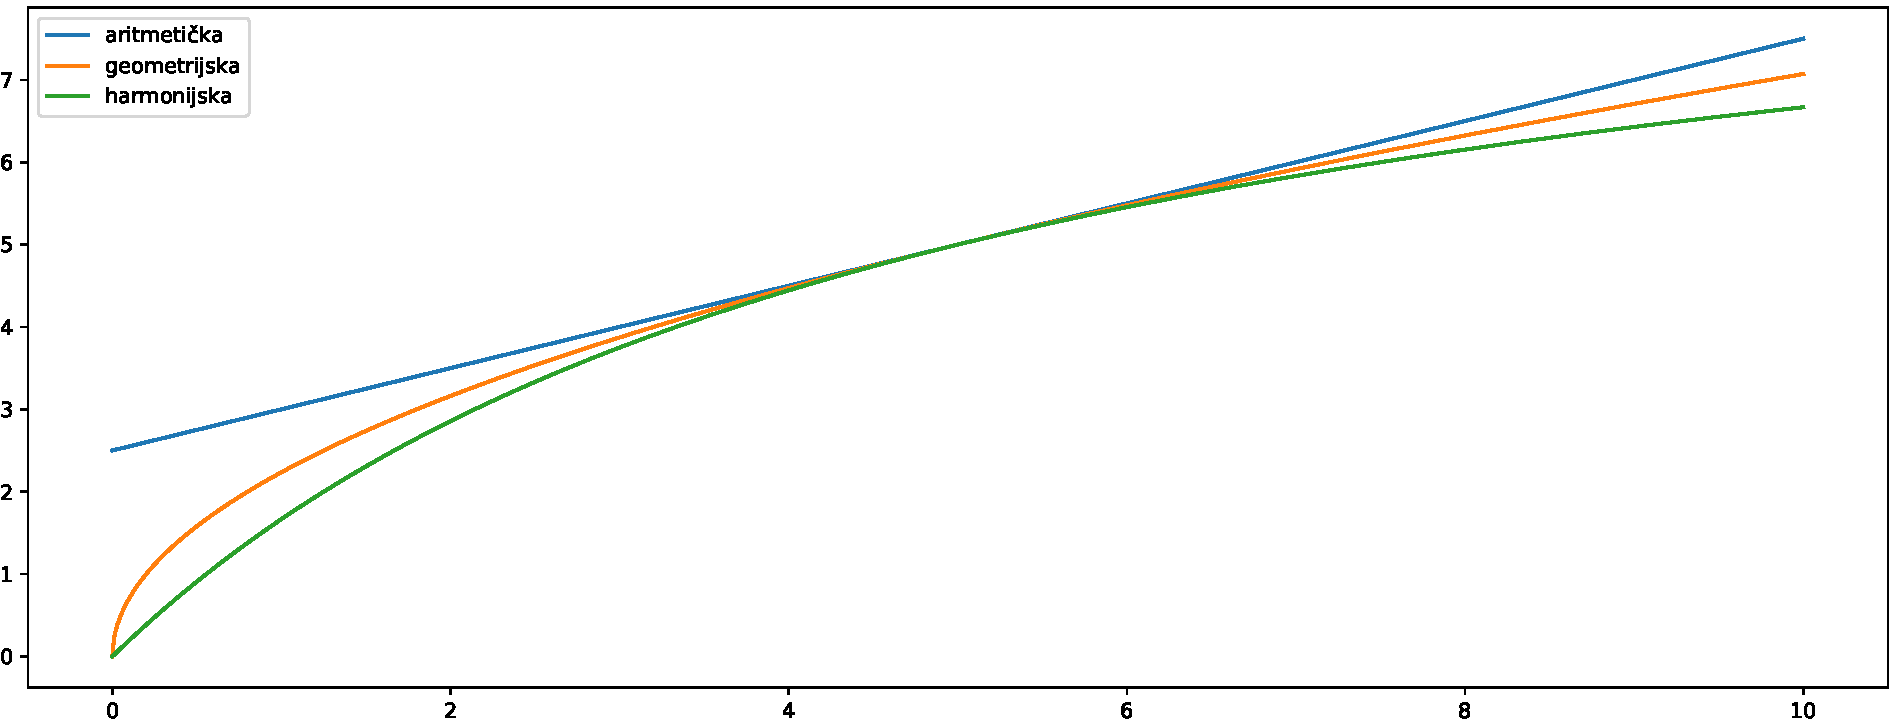
\includegraphics[width=\textwidth]{Pitagorine_sredine.pdf}
\centering
\caption{Pitagorine mjere za sredinu između dviju vrijednosti}
\label{fig:sredine}
\end{figure}

Mjere binarne klasifikacije mogu se primijeniti pri \textbf{višeklasnoj klasifikaciji}, no matrica zabune je dimenzija $C\times C$ gdje je $C$ broj klasa. Elementi matrice računaju se slično kao i kod binarne klasifikacije, ali za svaku klasu posebno.
\begin{align}
\label{eq:true_groups}
\begin{split}
\text{Stvarno pozitivni:} \quad TP_i &= \sum_{(x,y)\in\mathbb{D}} \mathbbm{1} \{h(x) =  C_i \wedge y = C_i \} \\
\text{Stvarno negativni:} \quad TN_i &= \sum_{(x,y)\in\mathbb{D}} \mathbbm{1} \{h(x) \neq C_i \wedge y \neq C_i \} \\
\text{Lažno pozitivni:} \quad FP_i &= \sum_{(x,y)\in\mathbb{D}} \mathbbm{1} \{h(x) = C_i \wedge y \neq C_i \} \\
\text{Lažno negativni:} \quad FN_i &= \sum_{(x,y)\in\mathbb{D}} \mathbbm{1} \{h(x) \neq C_i \wedge y = C_i \}
\end{split}
\end{align}

Za izračun složenijih mjera poput točnosti i \F1 mjere mora se računati prosjek po klasama. Koriste se dva pristupa računanju prosjeka: makro i mikro. \textbf{Makro prosjekom} prvo se izračunaju mjere svake klase naspram svih ostalih te se uzme njihov prosjek. Ova mjera pretpostavlja jednak utjecaj svih klasa nez obzira na njihovu veličinu \citep{ml_probabilistic}.
\begin{equation}
\begin{split}
Acc^M = \sum_{i=1}^K \frac{Acc_i}{K}
\end{split} \quad
\begin{split}
P^M = \sum_{i=1}^K \frac{P_i}{K}
\end{split} \quad
\begin{split}
R^M = \sum_{i=1}^K \frac{R_i}{K}
\end{split} \quad
\begin{split}
F_1^M = \sum_{i=1}^K \frac{F_{1;i}}{K}
\end{split}
\end{equation}

\textbf{Mikro prosjekom} prvo se zbroje matrice zabune po pojedinim klasama, a zatim se nad zbrojenom matricom računaju mjere. Na mikro prosjek više utječe veličina klasa i koristi se u nebalansiranim skupovima.

\begin{align}
\begin{split}
Acc^\mu &= \frac{\sum_i (TP_i+TN_i)}{\sum_i (TP_i+TN_i+FP_i+FN_i)} = Acc^M \\
FP = FN \implies P^\mu &= R^\mu = F_1^\mu = \frac{\sum_i TP_i}{\sum_i (TP_i+FP_i)}
\end{split}
\end{align}

\subsubsection{Pretraživanje po rešetci}
\label{sec:grid_search}
Najjednostavniji način za pretraživanje hiperparametara je pretraživanje po rešetci. Za svaki hiperparametar koji se optimizira definiraju se vrijednosti koje treba ispitati. Algoritam tada evaluira dani model za svaku kombinaciju hiperparametara i vraća kombinaciju ili model koji ostvaruje najbolje rezultate.

Iako se optimalni hiperparametri mogu nalaziti izvan zadanih skupova i neće biti pronađeni, postupak je brz i daje dovoljno dobre rezultate za praktičnu primjenu. Često je dovoljno da pronađe kombinaciju hiperparametara za koju model ne divergira niti prestaje učiti određen broj iteracija.

\subsection{Svojstva}
\label{sec:svojstva}

\subsubsection{Univerzalna aproksimacija}
Teorem univerzalne aproksimacije tvrdi da unaprijedna neuronska mreža može modelirati proizvoljnu Borel mjerljivu funkciju proizvoljno dobro uz nekoliko uvjeta: mora imati linearni izlaz, barem jedan nelinearni skriveni sloj koji koristi sažimajuću funkciju i "dovoljan" broj skrivenih neurona. Dakle, postoji arhitektura i postoje parametri kojima neuronska mreža može modelirati zadani podatkovni skup. No, teorem ne iskazuje kako doći do tih parametara što optimizaciju neuronske mreže čini vrlo teškom \citep{goodfellowbook}. 

\subsubsection{Reprezentacija dubinom}
Iako je prema teoremu univerzalne aproksimacije dovoljan jedan nelinearni skriveni sloj za predstavljanje proizvoljne Borel mjerljive funkcije, gornja granica veličine tog sloja je eksponencijalno velika naspram broja ulaza što je netraktabilno. Dodavanjem dubine moguće je iskoristiti pravilnosti u funkciji koja se aproksimira kako bi se smanjio potreban broj neurona. Primjer su funkcije simetrične oko neke osi. Ako skriveni slojevi mreže vrše preklapanje te funkcije preko same sebe, uzastopnim preklapanjem dobiva se sve jednostavnija funkcija. Preklapanje mogu vršiti po-dijelovima-linearne aktivacijske funkcije poput ReLU i Maxout. Dakako, ne postoji garancija da stvarna funkcija zadovoljava svojstvo simetrije, no u praksi dublje mreže generaliziraju bolje \citep{alexnet, highwaynet, resnet, densenet}. Postoje i druge interpretacije utjecaja dubine, poput svojstva dekompozicije zadatka na manje cjeline ili interpretacija neuronske mreže kao računalnog programa koje nadilaze temu ovog rada. \citep{goodfellowbook}

\iffalse %%%%%%%%%%%%%%%%%%%%%%%%%%%%%%%%%%%%%%%%%%%%%%%%%%%%%%%%%%%%%%%%%%%%%%%%%%%%
\todo{*VC dimenzija \citep{vc_dimension}}
\fi %%%%%%%%%%%%%%%%%%%%%%%%%%%%%%%%%%%%%%%%%%%%%%%%%%%%%%%%%%%%%%%%%%%%%%%%%%%%%%%%%

\iffalse %%%%%%%%%%%%%%%%%%%%%%%%%%%%%%%%%%%%%%%%%%%%%%%%%%%%%%%%%%%%%%%%%%%%%%%%%%%%
\subsubsection{*Kompresija podataka}
\todo{https://www.quantamagazine.org/new-theory-cracks-open-the-black-box-of-deep-learning-20170921/}
\fi %%%%%%%%%%%%%%%%%%%%%%%%%%%%%%%%%%%%%%%%%%%%%%%%%%%%%%%%%%%%%%%%%%%%%%%%%%%%%%%%%%

\subsubsection{Generalizacija}
\label{sec:generalizacija}
\todoimg{underfit-fit-overfit}

Model sa svojstvom generalizacije dobro modelira stvarnu funkciju te ispravno radi na neviđenim primjerima.

\todoimg{train-test U curve}

Ovo je posebno izraženo kod klasifikacije slika gdje za jednu generičku klasu (npr. automobil) postoji neprebrojivo mogućih slika s različitim modelom, bojom ili kutom gledanja automobila. No dostupno je svega nekoliko stotina tisuća primjera koji se smatraju reprezentativnim za tu klasu i njima se želi izgraditi klasifikator koji je robustan na većinu perturbacija slike.

\subsection{Problemi}
\subsubsection{Odabir hiperparametara}
Arhitektura, prijenosne funkcije i parametri definiraju neuronsku mrežu te njihov pravilan odabir značajno utječe na performanse neuronske mreže. Nažalost nije ih moguće optimalno odabrati u zatvorenom obliku, već se to svodi na problem pretraživanja kao što je pretraživanje po rešetci \secref{sec:grid_search}. Arhitekture mogu poprimiti vrlo složene oblike kao što je predstavljeno radovima \citet{highwaynet}, \citet{resnet}, \citet{densenet}, \citet{inceptionnet} i \citet{yolo} te se najčešće grade ručno s maksimalnom traktabilnom složenošću mreže. Detaljnije o odabiru aktivacijskih funkcija napisano je u poglavlju \ref{sec:aktivacijske_fje}.

\subsubsection{Nestajući gradijent}
\label{sec:nestajući_grad}
Prolaskom kroz duboku mrežu gradijent se množi matricama težina $\mat{W_i}$. Uzastopno množenje može dovesti do problema ako su svojstvene vrijednosti matrice udaljene od $\pm 1$. Rastavom matrice u umnošku ponovljenom $t$ puta \eqref{eq:vanish_grad} vidljiv je problem. Svojstvene vrijednosti veće od $1$ će rasti, a one manje od $1$ će se smanjivati. \citep{goodfellowbook}
\begin{equation}
\label{eq:vanish_grad}
\mat{W}^t = (\mat{V} diag(\mat{\lambda}) \mat{V}^{-1})^t = \mat{V} diag(\mat{\lambda})^t\mat{V}^{-1}
\end{equation}

Problem eksplodirajućeg gradijenta rješava se odrezivanjem gradijenta koji je prevelik. Problemu nestajućeg gradijenta moguće je pristupiti uvođenjem preskočnih veza u arhitekturu \citep{highwaynet,resnet,densenet} te odabirom aktivacijske funkcije s linearnim svojstvima \citep{elish}.

\iffalse %%%%%%%%%%%%%%%%%%%%%%%%%%%%%%%%%%%%%%%%%%%%%%%%%%%%%%%%%%%%%%%%%%%%%%%%
\subsubsection{*Neprijateljski primjeri}
\todo{Problem pretreniranosti + neprijateljski primjeri}

Vrlo složeni modeli, kao što su neuronske mreže, unatoč regularizaciji skloni su pretreniranju. \citep{intriguing_props}
\fi %%%%%%%%%%%%%%%%%%%%%%%%%%%%%%%%%%%%%%%%%%%%%%%%%%%%%%%%%%%%%%%%%%%%%%%%%%%%%

\chapter{Aktivacijske funkcije}
\label{sec:aktivacijske_fje}
Aktivacijska funkcija služi unošenju nelinearnosti u neuronsku mrežu i ima utjecaj na njeno učenje. Prilikom inferencije aktivacijske funkcija stvara nelinearnosti u decizijskoj granici koje su parametrizirane parametrima neurona na koji se primjenjuje. U slojevitim arhitekturama aktivacijske funkcije se primjenjuju uzastopno s različitim parametrima i vrše nelinearne projekcije iz jedne dimenzije u drugu.

Prilikom učenja neuronske mreže važan nam je utjecaj derivacije aktivacijske funkcije na gradijent pri širenju unatrag. Prolaskom unazad gradijent se množi s parametrima slojeva koji se mogu zapisati matricom težina $\mat{W}$. Uzastopnom primjenom matrica težina, ako su loše kondicionirane, može doći do "\textit{nestajanja}" ili "\textit{eksplozije}" gradijenta.

\section{Odabir aktivacijske funkcije}
Za odabir aktivacijske funkcije ne postoji jasno pravilo. U praksi se odabiru po empirijskim rezultatima i brzinom izvođenja. Iako neke funkcije imaju teorijski potkrijepljena svojstva to ih u praksi ne čini najboljima.

\todo{dokaz da su monotone fje dobre}

\subsection{Aktivacijske funkcije s učećim parametrima}
\todo{članak: učeći parametri u fjama (onaj stari)}

U radu \citet{trained_func} autori istražuju učeće aktivacijske funkcije ...

U radu TAF...

\todo{Spomeni i složenije metode: \citep{network_in_network}}

\subsection{Periodične aktivacijske funkcije}
\todo{članak: fourier mreža s periodičkim fjama}

Periodične aktivacijske funkcije stvaraju brojne lokalne optimume u funkciji gubitka koji otežavaju učenje neuronskih mreža. S obzirom da se mreže treniraju stohastičkim gradijentnim spustom većina lokalnih optimuma nije vidljiva i ublažava naglašenost lokalnih optimuma. Pri uporabi sinusoide autori pokazuju da će model konvergirati samo ako su težine inicijalizirane dovoljno malim vrijednostima da ulaz ne prelazi interval monotonosti sinusa $[-\frac{\pi}{2}, \frac{\pi}{2}]$. U usporedbi sinusoide s ograničenom sinusoidom na potpuno povezanom modelu pokazuje se nezamjetna razliku u performansama iako oko $40\%$ ulaza neurona završava izvan intervala monotonosti, što upućuje da modeli ne ovise o periodičnosti funkcije. U primjeni na rekurzivnim modelima ne ostvaruje konzistentnu prednost nad monotonim tangensom hiperbolnim zbog čega članak nije prošao postupak recenzije. \citep{taming_waves}

\todo{ostale reference iz taming the waves}

\section{Popularne aktivacijske funkcije}
U nastavku su navedene popularne aktivacijske funkcije koje je autor pronašao u literaturi i koje su isprobane u ovom radu. Funkcije su pasivne u smislu da ne sadrže učeće parametre te njihov izlaz ovisi isključivo o ulazu  u funkciju. Za svaku funkciju napisana je formula i iscrtan izgled funkcije i njene derivacije te navedena neka poznata svojstva.

\subsection{Funkcija identiteta}
\engl{Identity function}

\begin{figure}[H]
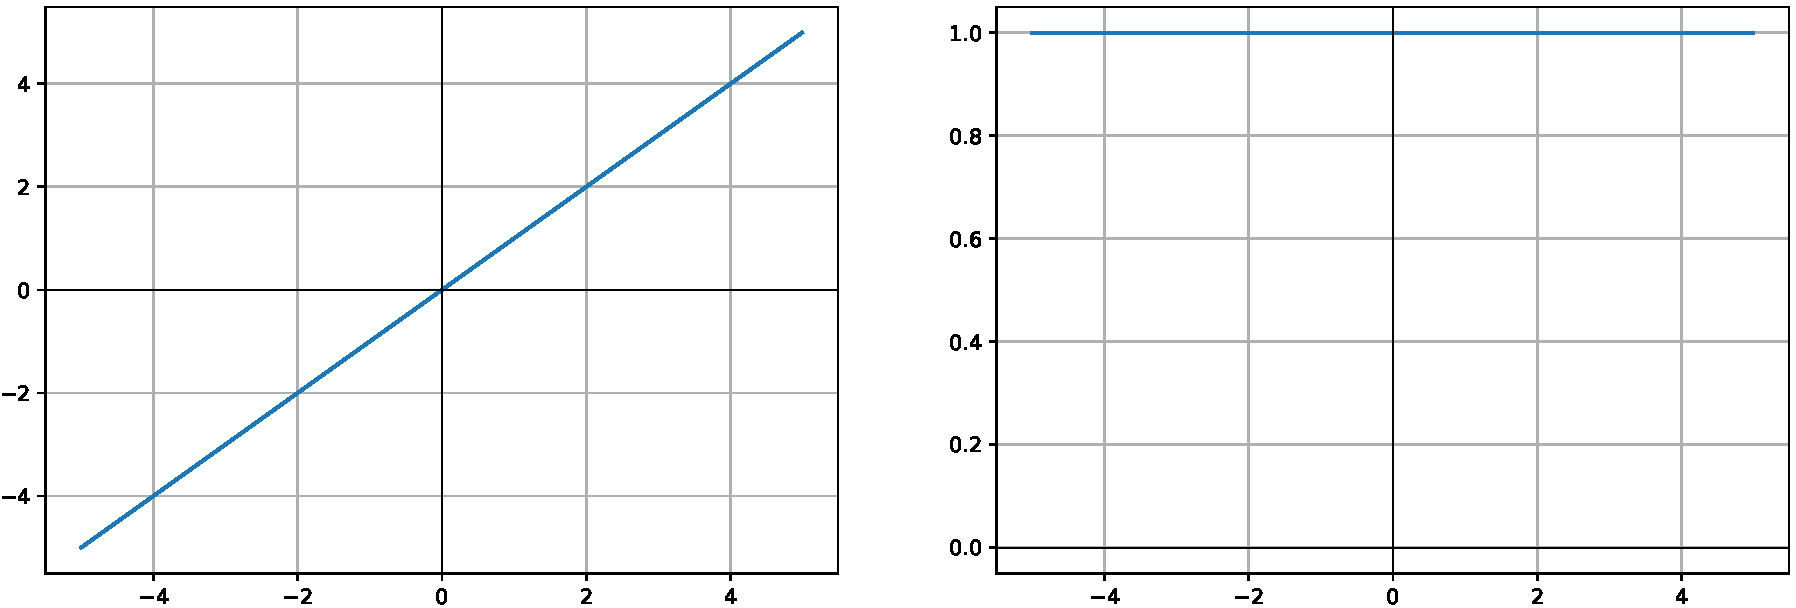
\includegraphics[width=\textwidth]{Identity.pdf}
\centering
\caption{Funkcija identiteta i njena derivacija}
\label{fig:identity}
\end{figure}

\begin{equation}
\begin{split}
f(x) = x
\end{split}
\qquad
\begin{split}
f'(x) = 1
\end{split}
\end{equation}

Funkcija identiteta je jednostavna i brza, no njome neuronska mreža može naučiti samo linearne funkcije. Ako se primijeni na dva uzastopna sloja neuronske mreže, konačna će funkcija ponovno biti linearna što znači da se mreža ne može koristiti na nelinearnim podatcima. Derivacija funkcije je konstanta $1$ što znači da je gradijent prolaskom kroz nju očuvan. Funkcija identiteta često se koristi kao funkcija aktivacijske sloja kod regresije, no u dubokim arhitekturama \citep{resnet,densenet} i novijim aktivacijskim funkcijama \citep{swish,elish} koristi se paralelno s nelinearnim funkcijama.
\begin{align}
\begin{split}
f_l(x) &= w_l \cdot x + b_l \\
f_1(f_2(x)) &= w_1 \cdot (w_2 \cdot x + b_2) + b_1 \\
&= \underline{w_1 \cdot w_2} \cdot x + \underline{w_1 \cdot b_2 + b_1} \\
&= w_{1,2} \cdot x + b_{1,2}
\end{split}
\end{align}

\subsection{Zglobnica ili ispravljena linearna jedinica (ReLU)}
\label{func:relu}
\engl{Rectified linear unit}

\begin{figure}[H]
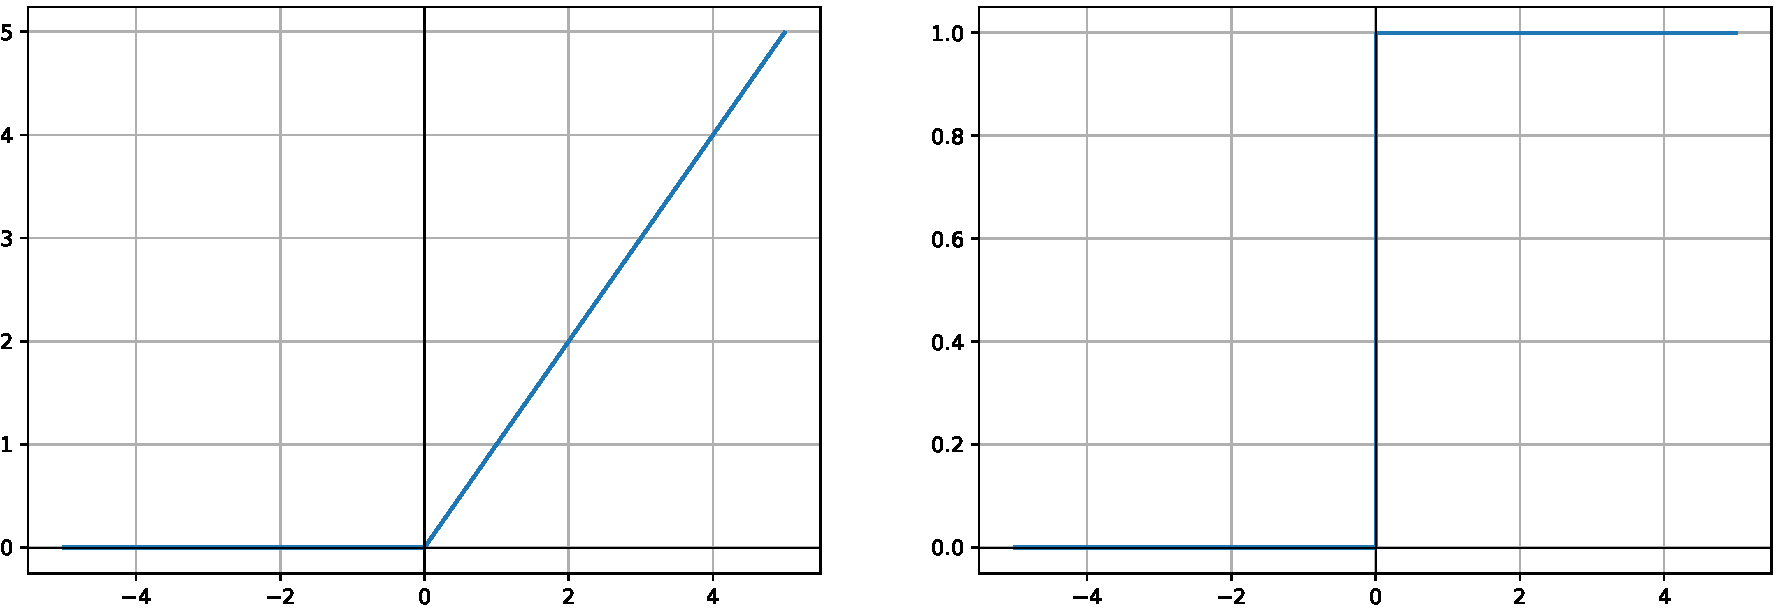
\includegraphics[width=\textwidth]{ReLU.pdf}
\centering
\caption{Funkcija ReLU i njena derivacija}
\label{fig:relu}
\end{figure}

\begin{equation}
\label{eq:relu}
\begin{split}
f(x) &= \begin{cases}
x,		& \text{ako } x > 0 \\
0,		& \otherwise
\end{cases} \\
&= max(0, x)
\end{split}
\qquad
\begin{split}
f'(x) = 
\begin{cases}
1,		& \text{ako } x > 0 \\
0,		& \otherwise
\end{cases}
\end{split}
\end{equation}

Funkcija ReLU svoje korijene povlači iz rada bioloških neurona, a u dubokom učenju je zamijenila dotadašnju sigmoidu i tangens hiperbolni. Zahvaljujući prizemljenosti na negativnoj domeni ReLU omogućava neuronskoj mreži učenje rijetke reprezentacije. Njihovim kombiniranjem u dubokoj mreži dobiva se model s eksponencijalno puno linearnih regija koje dijele zajedničke parametre \citep{relu_rbm}. Zahvaljujući linearnosti na pozitivnoj domeni funkcija ne doprinosi nestajanju ni eksploziji gradijenta, a sam izračun funkcije i derivacije je vrlo brz i efikasan. \citep{relu}

Problem u negativnoj domeni je mogućnost blokiranja gradijenta i neaktivnih neurona (mrtvi neuroni), no dok god postoji put kroz mrežu gdje su neuroni aktivni (u pozitivnoj domeni) učenje će raditi, što pokazuju i rezultati \citep{relu}. Drugi problem je u neograničenosti funkcije u pozitivnoj domeni, no on se rješava regularizacijom koja ograničava veličinu ulaza u neuron \citep{relu}.

\subsection{Propusna ispravljena linearna jedinica (LReLU)}
\engl{Leaky ReLU}

\begin{figure}[H]
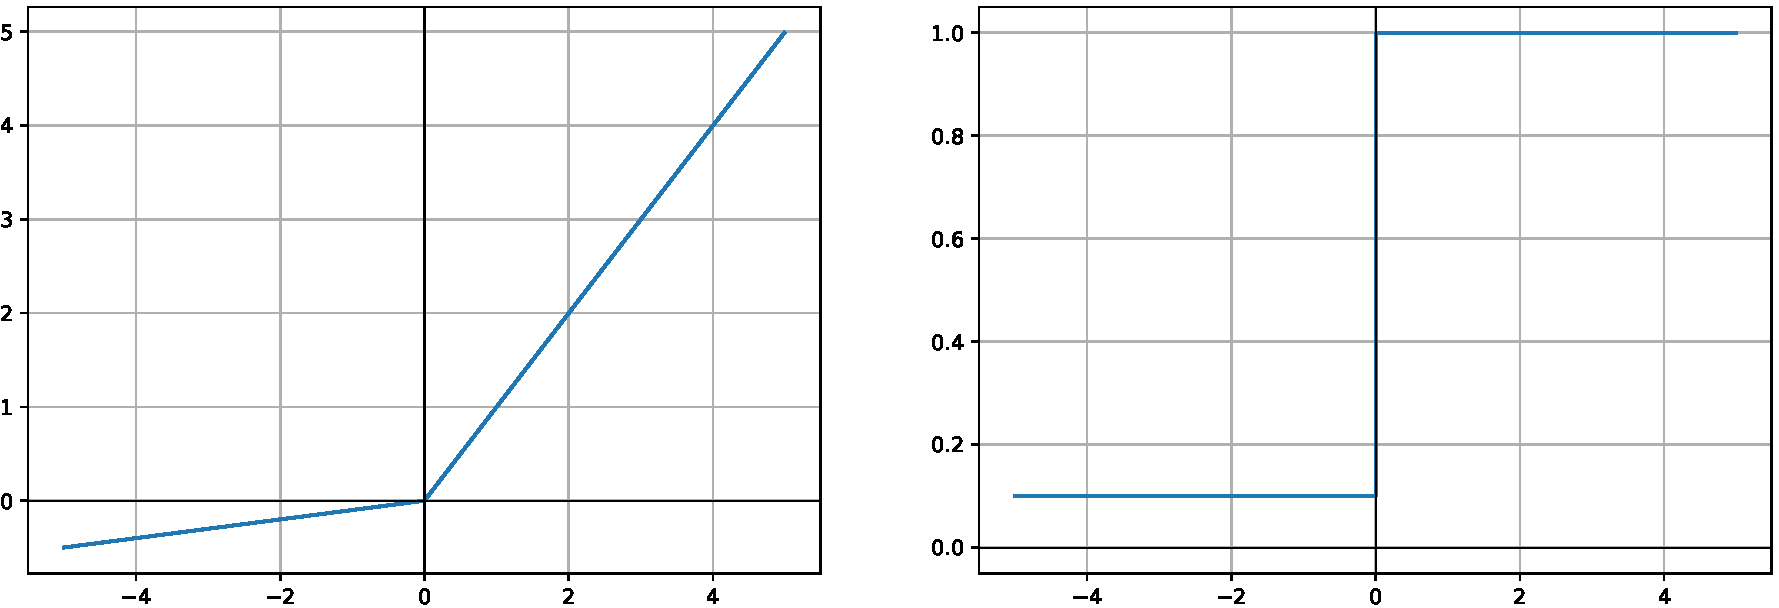
\includegraphics[width=\textwidth]{LReLU.pdf}
\centering
\caption{Funkcija LReLU i njena derivacija za $\alpha=0.1$}
\label{fig:lrelu}
\end{figure}

\begin{equation}
\label{eq:lrelu}
\begin{split}
f(x) &= \begin{cases}
x,			& \text{ako } x > 0 \\
\alpha x,	& \otherwise
\end{cases} \\
&= max(\alpha x, x)
\end{split}
\qquad
\begin{split}
f'(x) = 
\begin{cases}
1,		& \text{ako } x > 0 \\
\alpha,	& \otherwise
\end{cases}
\end{split}
\end{equation}

Problem funkcije ReLU \secref{func:relu} je što postoji mogućnost pojave mrtvih neurona, koji su uvijek u neaktivnom području i kroz njih ne teče gradijent. Taj problem efektivno smanjuje kapacitet modela pod cijenu nepotrebnog memorijskog opterećenja i smanjene brzine izvođenja. Iz navedenih razloga uvedena je propusna ReLU funkcija koja u "neaktivnom" području propušta mali gradijent. Rezultati na zadatku prepoznavanja govora pokazuju da je propusna ReLU funkcija ekvivalentna standardnom ReLU, no rezultati su prikazani na relativno plitkim arhitekturama (do 4 skrivena sloja). Tipična vrijednost parametra $\alpha$ je $0.01$. \citep{lrelu}

\iffalse %%%%%%%%%%%%%%%%%%%%%%%%%%%%%%%%%%%%%%%%%%%%%%%%%%%%%%%%%%%%%%%%%%%%%%%%%
\subsection{Nasumična ispravljena linearna jedinica (RReLU)}
\engl{Randomized leaky ReLU}

\todoimg{}

\begin{equation}
\begin{split}
f(x) &= 
\begin{cases}
x,			& \text{ako } x > 0 \\
\alpha x,	& \otherwise
\end{cases}
\end{split}
\qquad
\begin{split}
f'(x) = 
\begin{cases}
1,		& \text{ako } x > 0 \\
\alpha,	& \otherwise
\end{cases}
\end{split}
\end{equation}
\begin{equation}
\alpha \sim U(l,u),\quad l,u \in [0,1]
\end{equation}

\todo{koji problem rješava}
\todo{svojstva}
\todo{problemi}
\fi %%%%%%%%%%%%%%%%%%%%%%%%%%%%%%%%%%%%%%%%%%%%%%%%%%%%%%%%%%%%%%%%%%%%%%%%%%%%%%%%%%%%%

\subsection{Ispravljena linearna jedinica s pragom (ThReLU)}
\engl{Thresholded ReLU}

\begin{figure}[H]
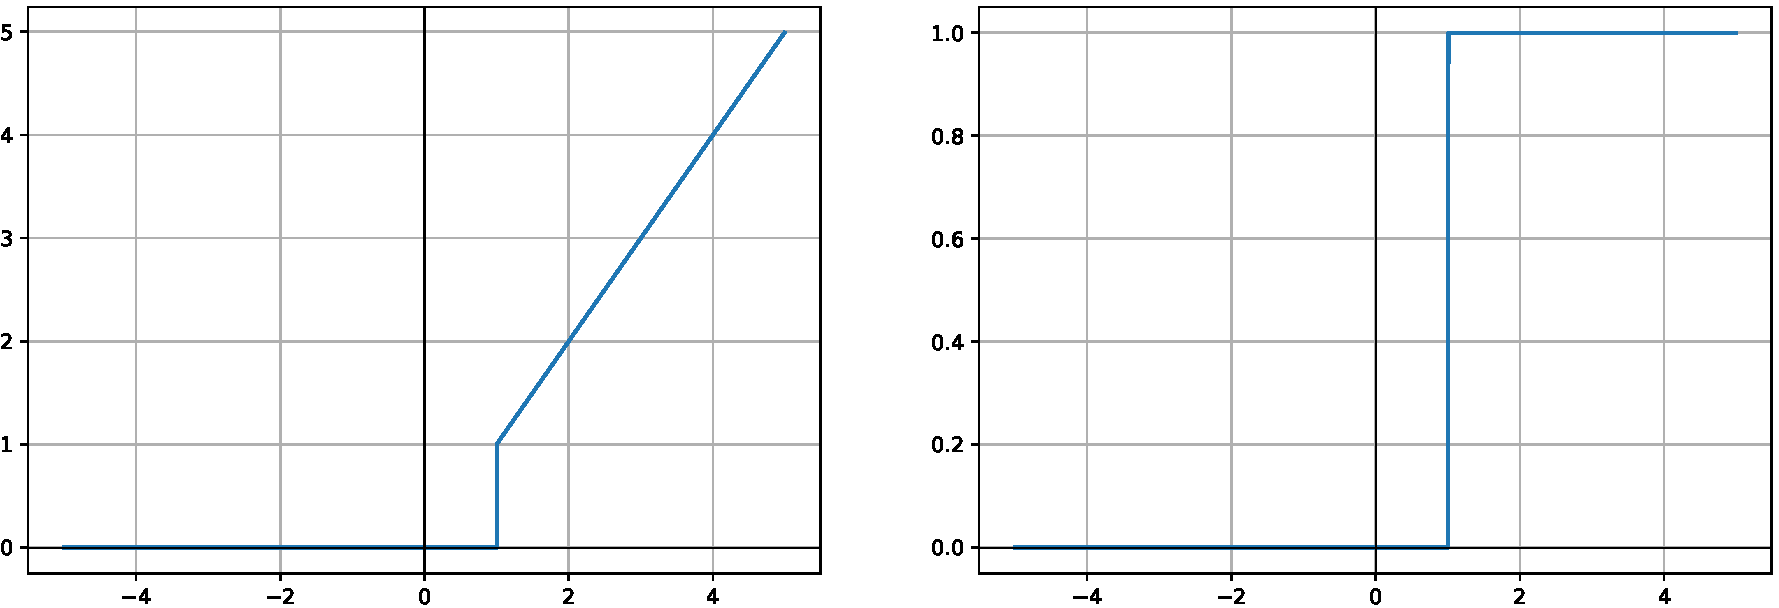
\includegraphics[width=\textwidth]{ThReLU.pdf}
\centering
\caption{Funkcija ThReLU i njena derivacija}
\label{fig:threlu}
\end{figure}

\begin{equation}
\label{eq:threlu}
\begin{split}
f(x) = 
\begin{cases}
x,		& \text{ako } x > \theta \\
0,		& \otherwise
\end{cases}
\end{split}
\qquad
\begin{split}
f'(x) = 
\begin{cases}
1,		& \text{ako } x > \theta \\
0,		& \otherwise
\end{cases}
\end{split}
\end{equation}

\todo{koji problem rješava}
\todo{svojstva}
\todo{problemi}



\iffalse %%%%%%%%%%%%%%%%%%%%%%%%%%%%%%%%%%%%%%%%%%%%%%%%%%%%%%%%%%%%%%%%%%%%%%%%%%%%%%%%
\subsection{(CReLU)}
\engl{Concatenated ReLU}

\todoimg{}

\begin{equation}
???
\end{equation}

\todo{koji problem rješava}
\todo{svojstva}
\todo{problemi}
\fi %%%%%%%%%%%%%%%%%%%%%%%%%%%%%%%%%%%%%%%%%%%%%%%%%%%%%%%%%%%%%%%%%%%%%%%%%%%%%%%%%%%%%

\subsection{Softplus}

\begin{figure}[H]
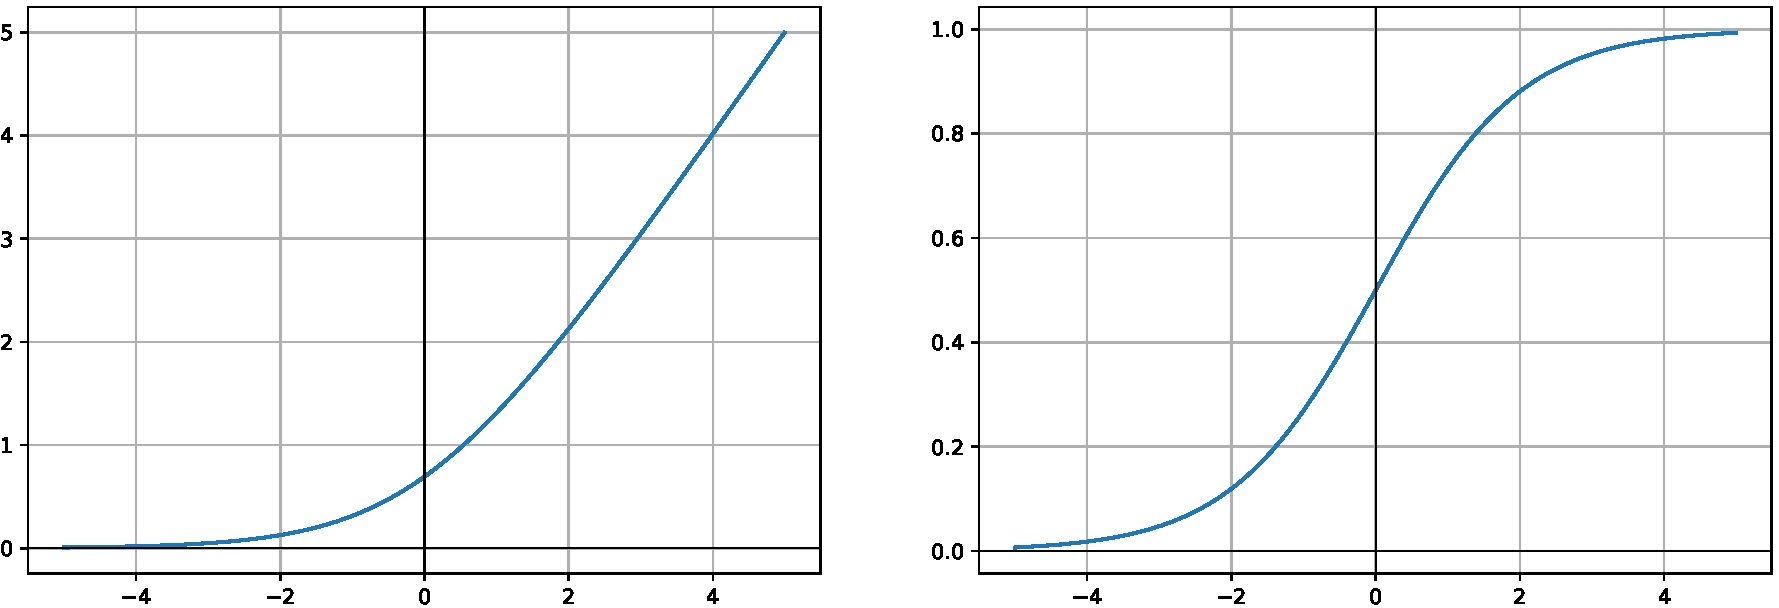
\includegraphics[width=\textwidth]{Softplus.pdf}
\centering
\caption{Softplus i njegova derivacija}
\label{fig:softplus}
\end{figure}

\begin{equation}
\label{eq:softplus}
\begin{split}
f(x) = log(1+e^x)
\end{split}
\qquad
\begin{split}
f'(x) = \frac{e^x}{1+e^x}
\end{split}
\end{equation}

Funkcija $Softplus$ je strogo pozitivna monotono rastuća glatka funkcija nalik na $ReLU$. Vrlo je bliska beskonačnom zbroju binomnih jedinica odmaknutih za $1$ koje se mogu koristiti u ograničenim Boltzmann-ovim strojevima. \citep{relu_rbm}
\begin{equation}
\sum_{i=1}^{\infty}\sigma(x-i+0.5) \approx log(1+e^x)
\end{equation}

U odnosu na $ReLU$, funkcija nema problem nestajućeg gradijenta jer propušta gradijent u negativnoj domeni i ostvaruje veće vrijednosti od $ReLU$. To je svojstvo posebna prednost nad $ReLU$ i sigmoidom pri korištenju tehnike Dropout kojom se blokira doprinos velikog broja neurona. Unatoč teoretskim prednostima funkcija rijetko postiže zadovoljive rezultate. \citep{softplus}

\todoimg{usporedba softplus i relu, možda zgodno za pokazati}

\iffalse %%%%%%%%%%%%%%%%%%%%%%%%%%%%%%%%%%%%%%%%%%%%%%%%%%%%%%%%%%%%%%%%%%%%%%%%%%%%%%%%
\subsection{Noisy softplus}

\todoimg{}

\begin{equation}
???
\end{equation}

\todo{koji problem rješava}
\todo{svojstva}
\todo{problemi}
\fi %%%%%%%%%%%%%%%%%%%%%%%%%%%%%%%%%%%%%%%%%%%%%%%%%%%%%%%%%%%%%%%%%%%%%%%%%%%%%%%%%%%%

\subsection{Eksponencijalno-linearna jedinica (ELU)}
\label{func:elu}
\engl{Exponential linear unit}

\begin{figure}[H]
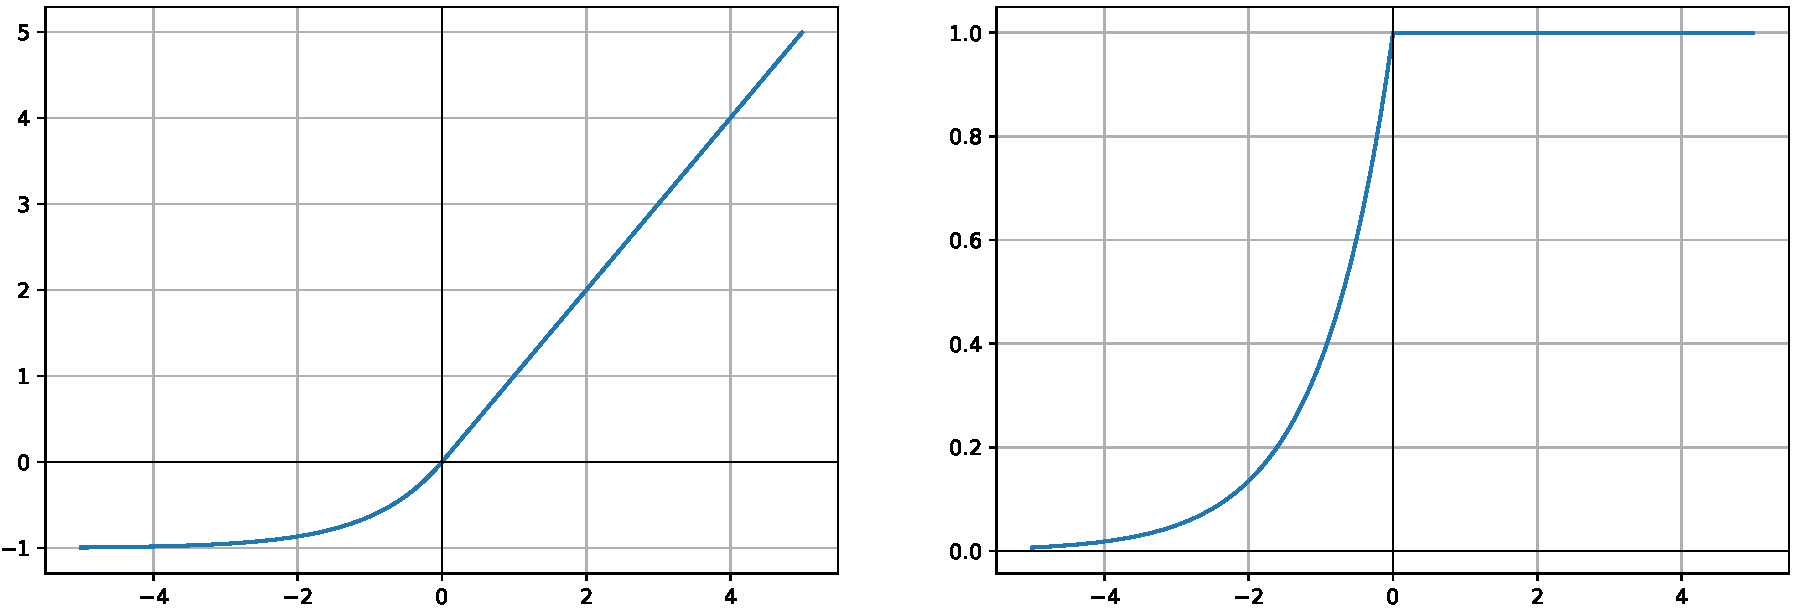
\includegraphics[width=\textwidth]{ELU.pdf}
\centering
\caption{Funkcija ELU i njena derivacija}
\label{fig:elu}
\end{figure}

\begin{equation}
\label{eq:elu}
\begin{split}
f(x) = 
\begin{cases}
x,					& \text{ako } x > 0 \\
\alpha (e^x - 1),	& \otherwise
\end{cases}
\end{split}
\qquad
\begin{split}
f'(x) = 
\begin{cases}
1,	 		& \text{ako } x > 0 \\
\alpha e^x,	& \otherwise
\end{cases}
\end{split}
\end{equation}

Funkcija $ELU$ je linearna na pozitivnoj domeni, a u negativnoj domeni postepeno prelazi u zasićenje. Uvedena je kako bi umanjila efekt otklona izlaza neurona, koja nastaje kada je srednja vrijednost izlaza otklonjena od $0$. Aktivacije koje nisu centrirane usporavaju učenje mreže i stoga ih je potrebno centrirati. Jedan pristup je centriranje normalizacijom grupa, a alternativni je odabirom aktivacijske funkcije. $ReLU$ nije centriran jer je u pozitivnoj domeni linearan, a u negativnoj $0$. Tangens hiperbolni je primjer centrirane funkcije. $ELU$ je djelom linearan pa nema problem nestajućeg gradijenta te brže prelazi u zasićenje i time smanjuje razlike između neaktivnih neurona za različite ulazne argumente što ga čini otpornim na šum. Hiperparametar $\alpha$ određuje negativnu vrijednost zasićenja i tipično se postavlja na $1$. Funkcija postiže bolje rezultate od $ReLU$ s normalizacijom grupe. Kada se koristi s normalizacijom grupe ostvaruje nešto lošije rezultate, no i dalje bolje od $ReLU$ i izvedenica. \citep{elu}

\subsection{Skalirana eksponencijalno-linearna jedinica (SELU)}
\engl{Scaled exponential linear unit}

\begin{figure}[H]
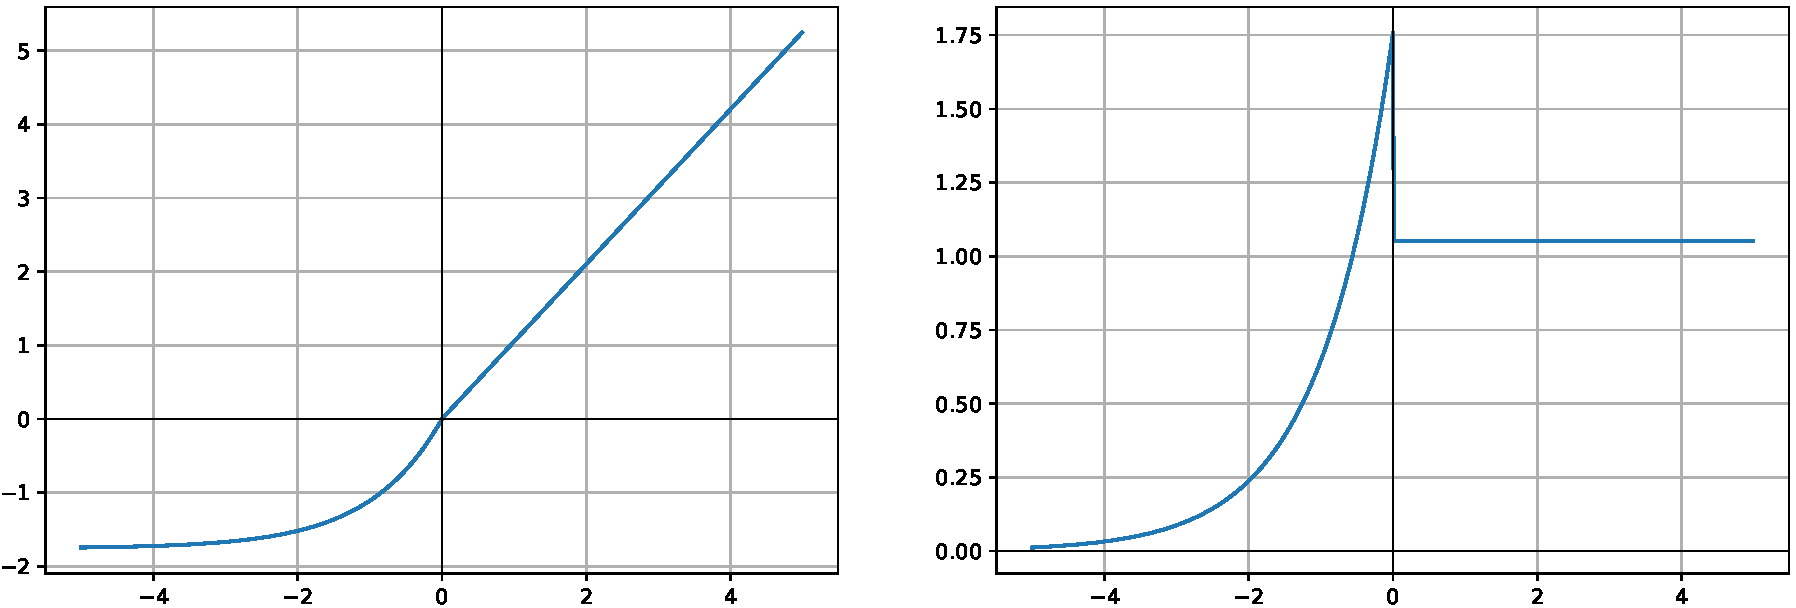
\includegraphics[width=\textwidth]{SELU.pdf}
\centering
\caption{Funkcija SELU i njena derivacija}
\label{fig:selu}
\end{figure}

\begin{equation}
\label{eq:selu}
\begin{split}
f(x) = \lambda
\begin{cases}
x,					& \text{ako } x > 0 \\
\alpha (e^x - 1),	& \otherwise
\end{cases}
\end{split}
\qquad
\begin{split}
f'(x) = \lambda
\begin{cases}
1,	 		& \text{ako } x > 0 \\
\alpha e^x,	& \otherwise
\end{cases}
\end{split}
\end{equation}

Aktivacijska funkcija $SELU$ izgrađena je za ostvarivanje samo-normalizirajuće neuronske mreže kojom je moguće izgraditi duboke potpuno povezane modele bez potrebe za eksplicitnim tehnikama normalizacije. Funkcija naslijeđuje svojstvo otpornosti na nestajuće i eksplodirajuće gradijente od funkcije $ELU$ \secref{func:elu}. Primjenom funkcije na mreži s prilagođenom inicijalizacijom i regularizacijom ostvaruju se rezultati bolji od ekvivalentnih mreža s primjenjenim tehnikama normalizacije (normalizacija težina, slojeva ili grupom) te specijaliziranih mreža (HighwayNet \citep{highwaynet}, ResNet \citep{resnet}) na brojnim podatkovnim skupovima. Performanse samo-normalizirajućih mreža potkrijepljene su teorijom te su definirane vrijednosti parametara $\alpha \approx 1.6733$ i $\lambda \approx 1.0507$ za normalizirane ulaze u sloj. \citep{selu}

\iffalse %%%%%%%%%%%%%%%%%%%%%%%%%%%%%%%%%%%%%%%%%%%%%%%%%%%%%%%%%%%%%%%%%%%%%%%%%%%%%%%
\subsection{(GELU)}
\engl{Gaussian error linear unit}

\todoimg{}

\todo{koji problem rješava}
\todo{svojstva}
\todo{problemi}
\fi %%%%%%%%%%%%%%%%%%%%%%%%%%%%%%%%%%%%%%%%%%%%%%%%%%%%%%%%%%%%%%%%%%%%%%%%%%%%%%%%%%%%

\subsection{Swish}
\label{func:swish}

\begin{figure}[H]
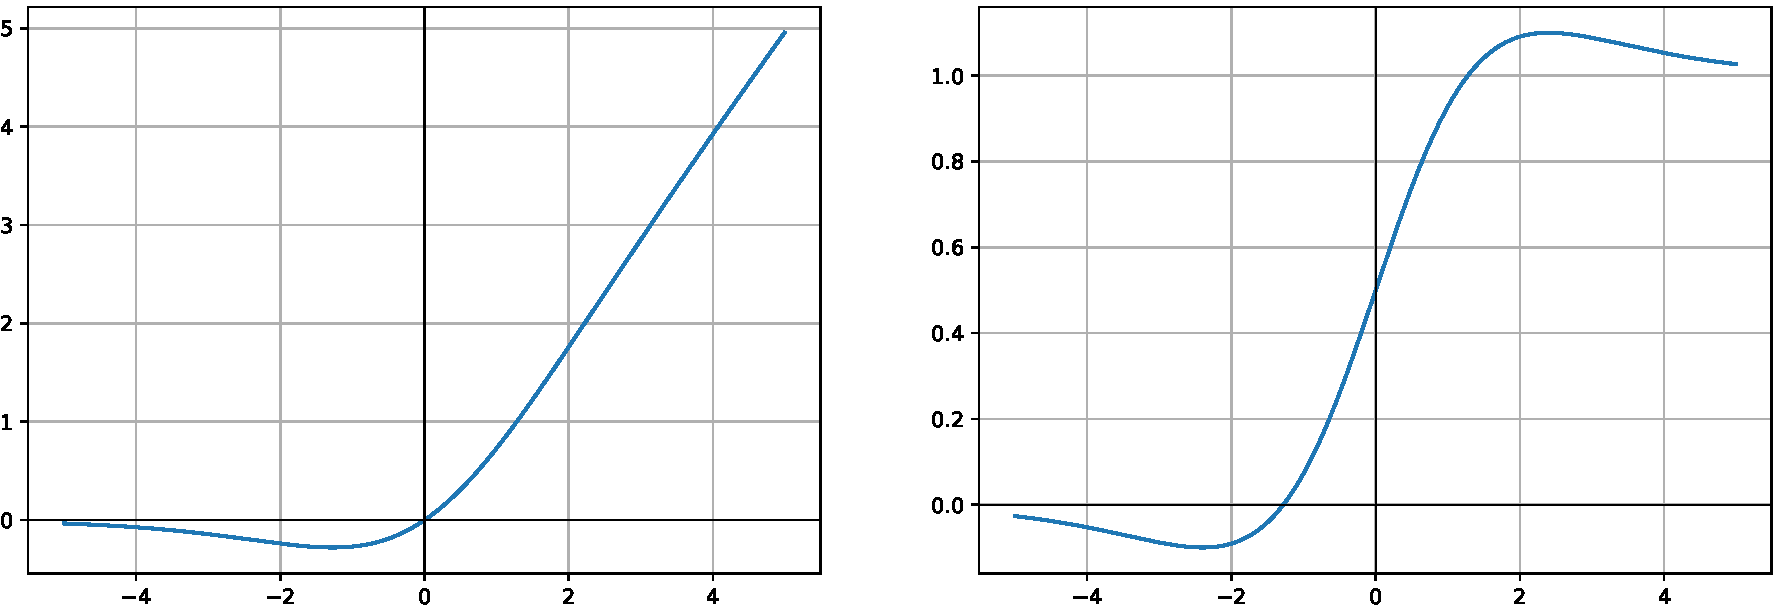
\includegraphics[width=\textwidth]{Swish.pdf}
\centering
\caption{Funkcija Swish i njena derivacija}
\label{fig:swish}
\end{figure}

\begin{equation}
\label{eq:swish}
\begin{split}
f(x) = x \cdot \sigma(\beta x)
\end{split}
\qquad
\begin{split}
f'(x) = \sigma(\beta x) \cdot (1 + \beta x \cdot (1-\sigma(\beta x))
\end{split}
\end{equation}
\begin{equation*}
\beta \text{ može biti definiran ili je učeći parametar}
\end{equation*}

Funkcija Swish je pronađena pretragom temeljenom na potpornom učenju. Funkcija zadovoljava strukturu kompozicije binarne (umnožak) i dviju unarnih operacija (identitet i sigmoida). Ispitivanje funkcije na nekoliko podatkovnih skupova i na nekoliko dubokih arhitektura s preskočnim vezama ostvaruje konzistentno bolje rezultate u odnosu na nekoliko dotadašnjih najboljih funkcija bez mijenjanja originalnih hiperparametara. Udubina funkcije na negativnoj domeni pokazuje se važnom jer se većina izlaza nalazi upravo tamo. Parametar $\beta$ interpolira funkciju između linearne funkcije ($\beta=0$) i funkcije $ReLU$ ($\beta \rightarrow \infty$). \citep{swish}

\subsection{ELiSH}
\label{func:elish}
\engl{Exponential Linear Sigmoid Squashing}

\begin{figure}[H]
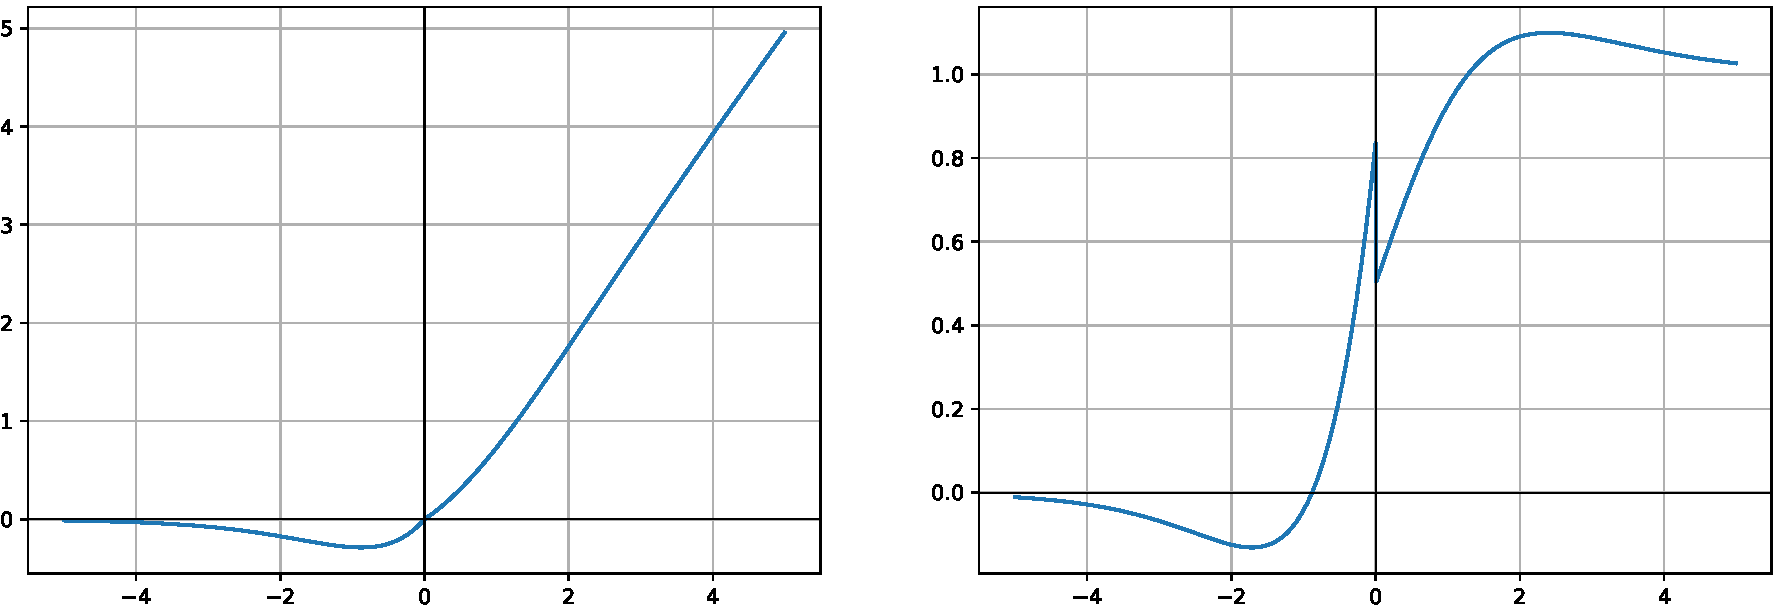
\includegraphics[width=\textwidth]{ELiSH.pdf}
\centering
\caption{Funkcija ELiSH i njena derivacija}
\label{fig:elish}
\end{figure}

\begin{equation}
\begin{split}
&f(x) = 
	\begin{cases}
		swish(x), \quad x \geq 0 \\
		ELU(x) \cdot \sigma(x), \quad \otherwise
	\end{cases} \\
&f'(x) =
	\begin{cases}
		swish'(x), \quad x \geq 0 \\
		\sigma(x) \cdot (ELU'(x) + ELU(x) \cdot (1-\sigma(x)), \quad \otherwise
	\end{cases}
\end{split}
\end{equation}

Ova funkcija i njena brža aproksimacija \textit{Tvrdi ELiSH} su kompozicije funkcija, različito definirane na pozitivnoj i negativnoj domeni. ELiSH pozitivnu domenu nasljeđuje od funkcije Swish \eqref{eq:swish}, a negativna je umnožak funkcije ELU \eqref{eq:elu} i sigmoide \eqref{eq:sigmoid}. Obje funkcije su ručno izgrađene s ciljem iskorištavanja dobrog prijenosa informacije koji ostvaruju funkcije Swish i sigmoida te sprečavanjem nestajućeg gradijenta pomoću linearne komponente u funkciji Swish. \citep{elish}

\subsection{Tvrdi ELiSH}
\label{func:hard_elish}
\engl{Hard ELiSH}

\begin{figure}[H]
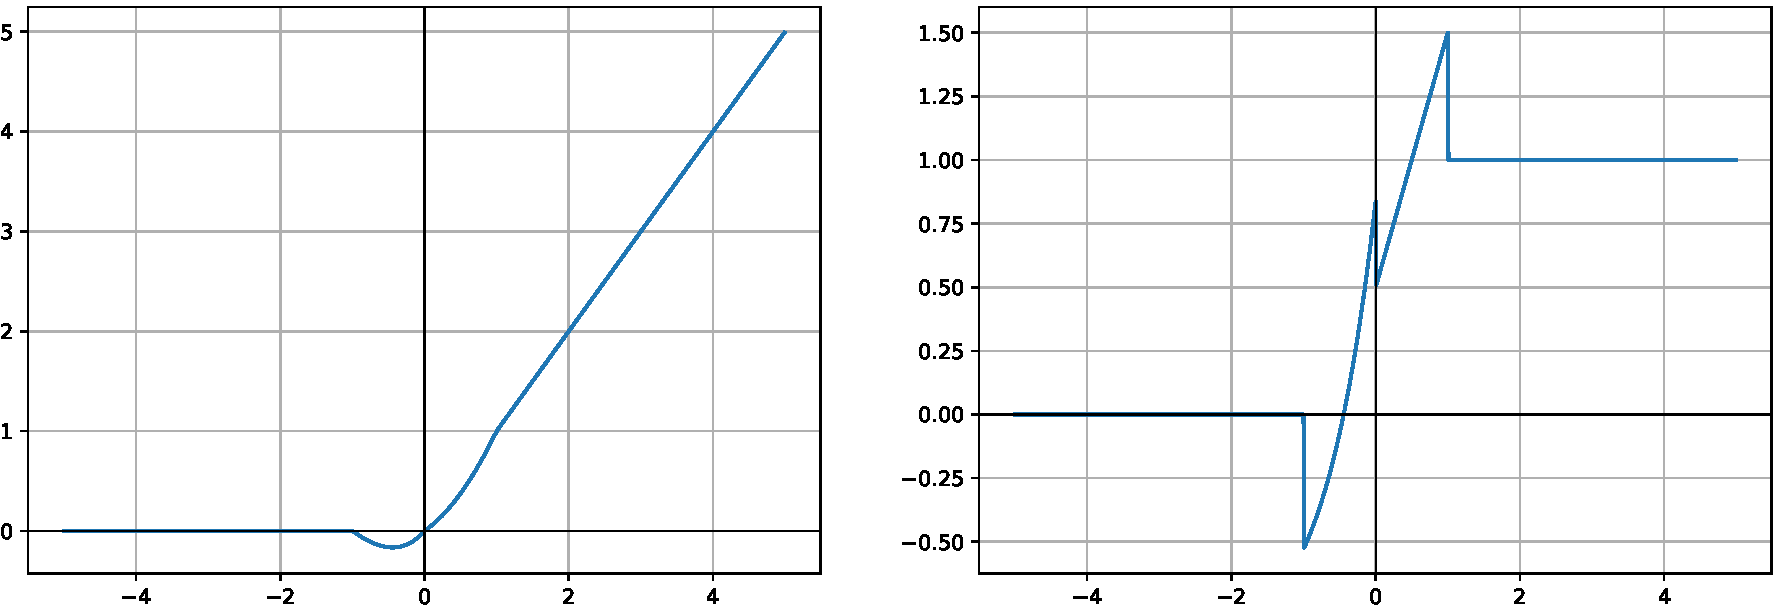
\includegraphics[width=\textwidth]{Hard_ELiSH.pdf}
\centering
\caption{Funkcija Tvrdi ELiSH i njena derivacija}
\label{fig:hard_elish}
\end{figure}

\begin{equation}
\begin{split}
&f(x) =
	\begin{cases}
		x \cdot a(x), \quad x \geq 0 \\
		ELU(x) \cdot a(x), \quad \otherwise
	\end{cases} \\
&f'(x) = \begin{cases}
	a(x) + x \cdot a'(x), \quad x \geq 0 \\
	ELU'(x) \cdot a(x) + x \cdot ELU(x) \cdot a'(x), \quad \otherwise
\end{cases}
\end{split}
\end{equation}

\begin{equation}
\begin{split}
&a(x) = \max(0, \min(1, \frac{x+1}{2})) \approx HardSigmoid(x) \\
&a'(x) =
\begin{cases}
	0.5, \quad |x| \leq 1 \\
	0, \quad \otherwise
\end{cases}	
\end{split}
\end{equation}

Ova funkcija je aproksimacija funkcije ELiSH opisane u poglavlju \ref{func:elish}. Uvedena je za potrebe bržeg izvođenja sigmoide i nasljeđuje svojstva ELiSH funkcije. \citep{elish}

\subsection{Ograničena ispravljena linearna jedinica (ReLU-n)}
\label{func:relun}

\begin{figure}[H]
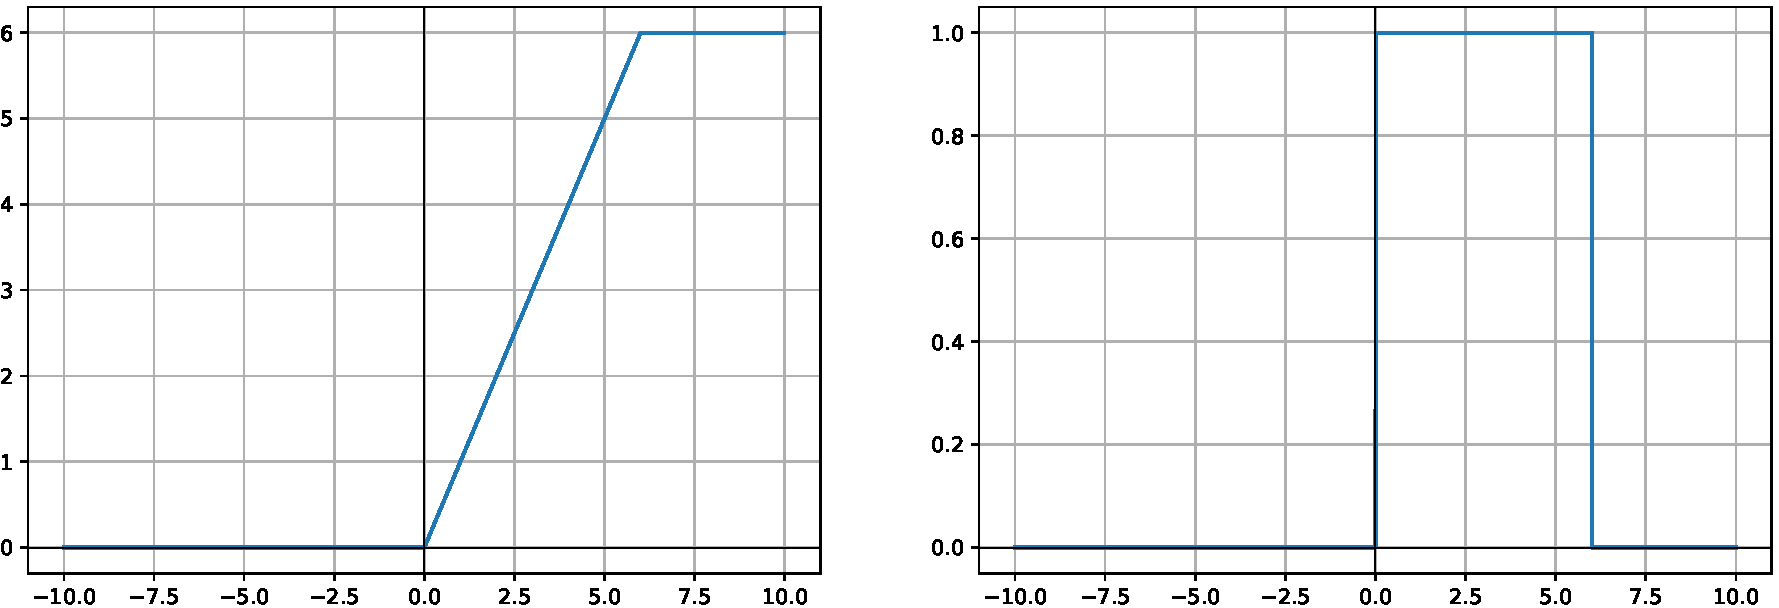
\includegraphics[width=\textwidth]{ReLU6.pdf}
\centering
\caption{Funkcija ReLU6 i njena derivacija}
\label{fig:relu6}
\end{figure}

\begin{equation}
\label{eq:relun}
\begin{split}
f(x) &= \begin{cases}
0,		& \text{ako } x < 0 \\
x,		& \text{ako } x \in [0, n] \\
n,		& \otherwise
\end{cases} \\
&= min(n, max(0, x))
\end{split}
\qquad
\begin{split}
f'(x) = 
\begin{cases}
1,		& \text{ako } x \in [0, n] \\
0,		& \otherwise
\end{cases}
\end{split}
\end{equation}
\begin{equation*}
n \in \realnum
\end{equation*}

Ograničena ReLU funkcija uvedena je kako bi ograničeni Boltzmann-ov stroj \engl{Restricted Boltzmann machine} brže naučio rijetke značajke, koje kasnije ugađa konvolucijski klasifikator. Za razliku od ReLU koji se može interpretirati kao kompozicija beskonačno mnogo identičnih Bernoullijevih jedinica translatiranih po domeni, ograničeni ReLU interpretira se kao kompozicija $n$ Bernoullijevih jedinica. Za vidljivi sloj autori koriste ReLU1, a za skrivene slojeve ReLU6. \citep{relu6}

S obzirom da je ReLUn neuron aktivan samo na relativno uskoj regiji u pozitivnoj domeni, postoji opasnost od pojave mrtvih neurona (kroz koje ne prolazi gradijent). Idealna regija je $<0,n>$ jer  je u njoj neuron aktivan, a učenjem se može specijalizirati približavanjem zasićenju i stvoriti rijetke reprezentacije. Stoga je potrebno koristiti regularizaciju te pažljivu inicijalizaciju parametara.

\subsection{Sigmoida ($\sigma $)}
\engl{Sigmoid}

\begin{figure}[H]
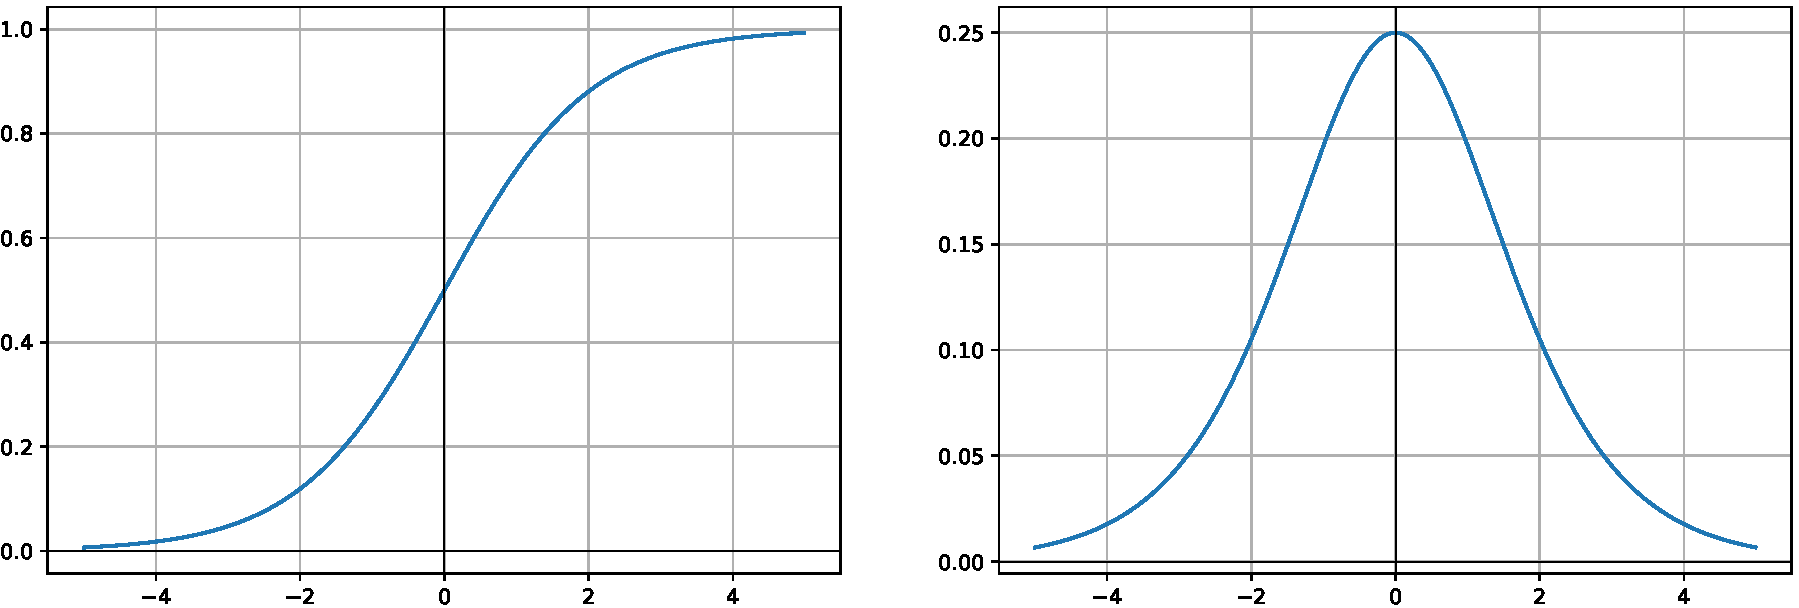
\includegraphics[width=\textwidth]{Sigmoid.pdf}
\centering
\caption{Sigmoida i njena derivacija}
\label{fig:sigmoid}
\end{figure}

\begin{equation}
\label{eq:sigmoid}
\begin{split}
f(x) = \frac{1}{1+e^{-x}}
\end{split}
\qquad
\begin{split}
f'(x) = \sigma(x)(1-\sigma(x))
\end{split}
\end{equation}

\todo{koji problem rješava}
\todo{svojstva}
\todo{problemi}

\subsection{Tvrda sigmoida}
\engl{Hard sigmoid}

\begin{figure}[H]
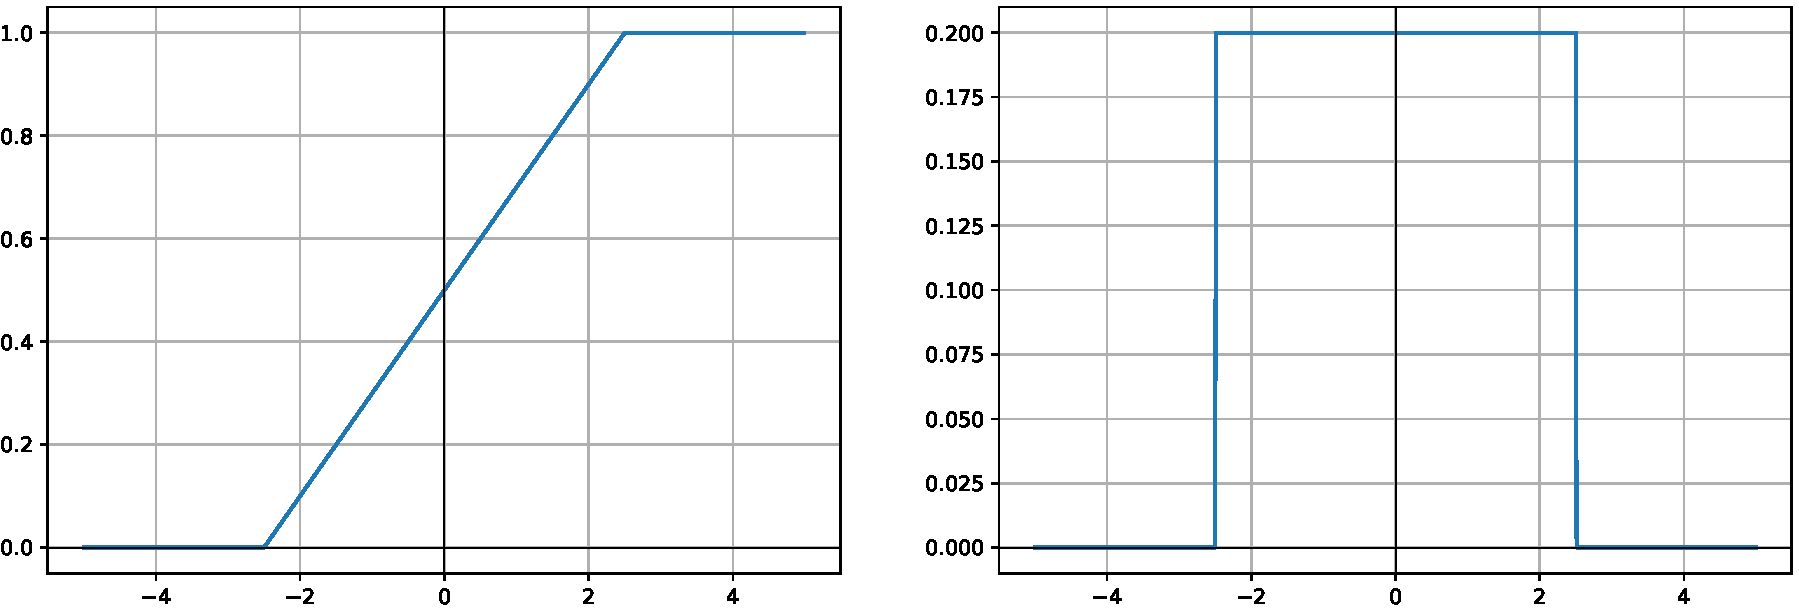
\includegraphics[width=\textwidth]{Hard_sigmoid.pdf}
\centering
\caption{Tvrda sigmoida i njena derivacija}
\label{fig:hard_sigmoid}
\end{figure}

\begin{equation}
\label{eq:hsigmoid}
\begin{split}
f(x) = min(1,\ max(0,\ 0.2x + 0.5))
\end{split}
\qquad
\begin{split}
f'(x) = 
\begin{cases}
0.2,	 		& \text{ako } |x| \leq 2.5 \\
0,	& \text{inače}
\end{cases}
\end{split}
\end{equation}

\todo{koji problem rješava}
\todo{svojstva}
\todo{problemi}

\subsection{Tangens hiperbolni (tanh)}
\label{func:tanh}

\begin{figure}[H]
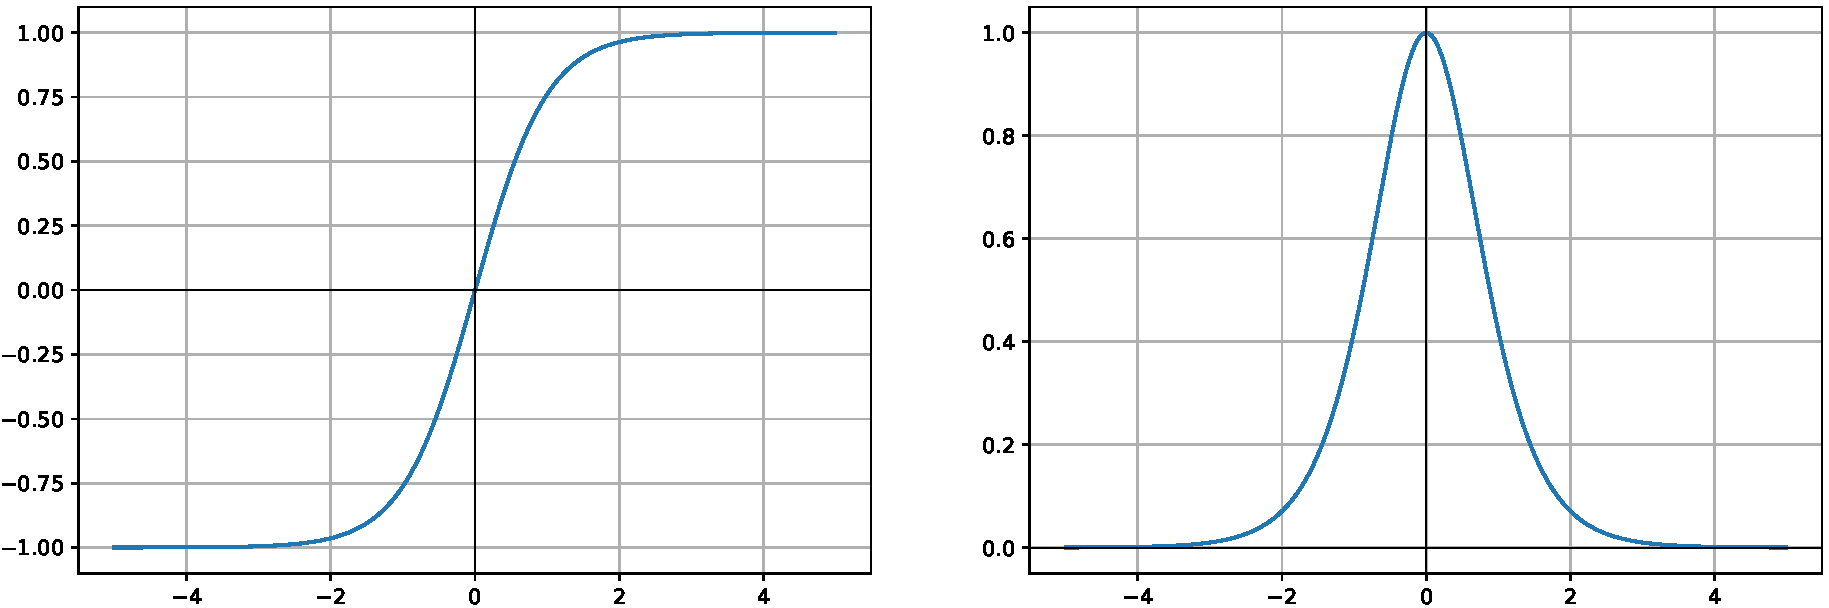
\includegraphics[width=\textwidth]{tanh.pdf}
\centering
\caption{Funkcija tanh i njena derivacija}
\label{fig:tanh}
\end{figure}

\begin{equation}
\label{eq:tanh}
\begin{split}
f(x) = \frac{e^x - e^{-x}}{e^x + e^{-x}}
\end{split}
\qquad
\begin{split}
f'(x) = 1 - tanh^2(x)
\end{split}
\end{equation}

\todo{koji problem rješava}
\todo{svojstva}
\todo{problemi}

\subsection{Tvrdi tangens hiperbolni}
\engl{Hard tanh}

\begin{figure}[H]
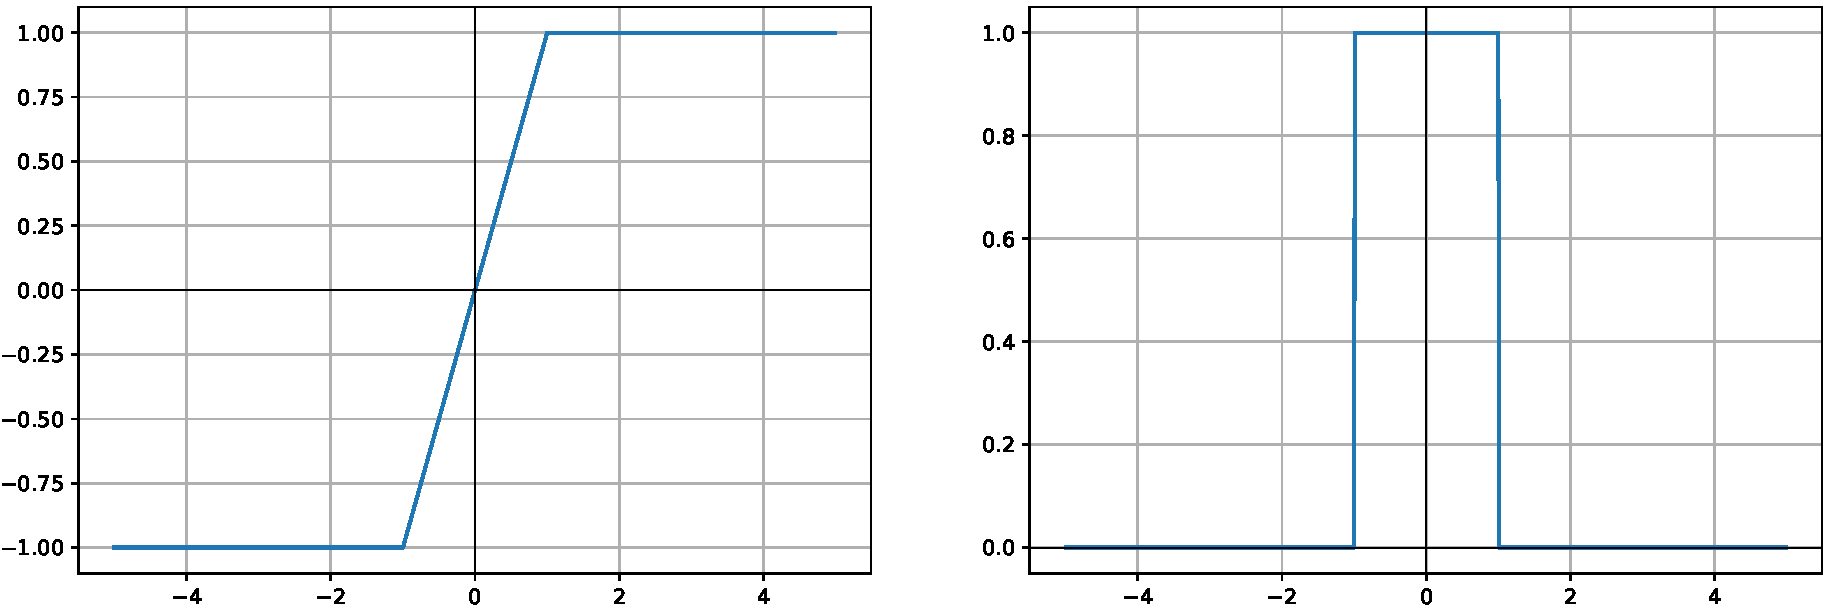
\includegraphics[width=\textwidth]{Hard_tanh.pdf}
\centering
\caption{Tvrdi tanh i njegova derivacija}
\label{fig:hard_tanh}
\end{figure}

\begin{equation}
\label{eq:htanh}
\begin{split}
f(x) =
\begin{cases}
-1,	 		& \text{ako } x < 1 \\
x,	 		& \text{ako } |x| \leq 1 \\
1,	& \text{inače}
\end{cases}
\end{split}
\qquad
\begin{split}
f'(x) =
\begin{cases}
0,	 		& \text{ako } x < 1 \\
1,	 		& \text{ako } |x| \leq 1 \\
0,	& \text{inače}
\end{cases}
\end{split}
\end{equation}

Tvrdi tangens hiperbolni je linearizirana aproksimacija tangensa hiperbolnog korištena u radu \citet{collobert_phd}. Iako nema glatkoću originalne funkcije i ne propušta gradijent izvan intervala $[-1,1]$, jednako dobro pomaže generalizaciji mreže. Koristan je zbog veće brzine izvođenja funkcije i derivacije u odnosu na tangens hiperbolni.

\subsection{Racionalna aproksimacija tanh}
\engl{Rational tanh}

\begin{figure}[H]
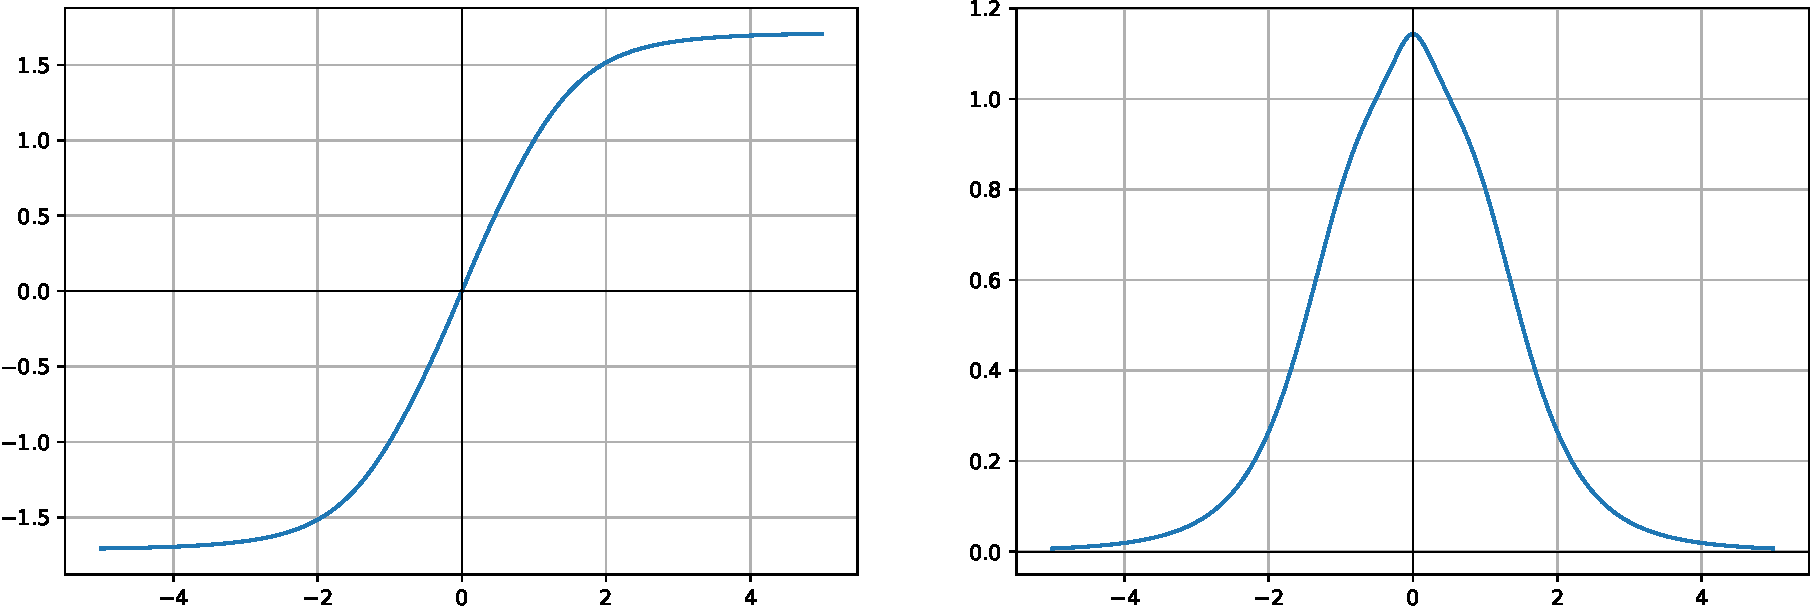
\includegraphics[width=\textwidth]{Rational_tanh.pdf}
\centering
\caption{Racionalni tanh i njegova derivacija}
\label{fig:rational_tanh}
\end{figure}

\begin{align}
\label{eq:rattanh}
\begin{split}
f(x) &= 1.7159 \cdot tanh^*(\frac{2}{3}x), \quad
tanh^*(x) = sgn(x)(1 - \frac{1}{1 + |x| + x^2 + 1.41645 \cdot x^4}) \\
f'(x) &= 1.7159 \cdot \frac{2}{3} \cdot tanh^{*'}(\frac{2}{3}x), \quad
tanh^{*'}(x) = \frac{1+sgn(x) \cdot (2x + 4 \cdot 1.41645 \cdot x^3)}{(1 + |x| + x^2 + 1.41645 \cdot x^4)^2}
\end{split}
\end{align}

\todo{koji problem rješava}
\todo{svojstva}
\todo{problemi}

\subsection{Ispravljeni tanh}
\engl{Rectified tanh}

\begin{figure}[H]
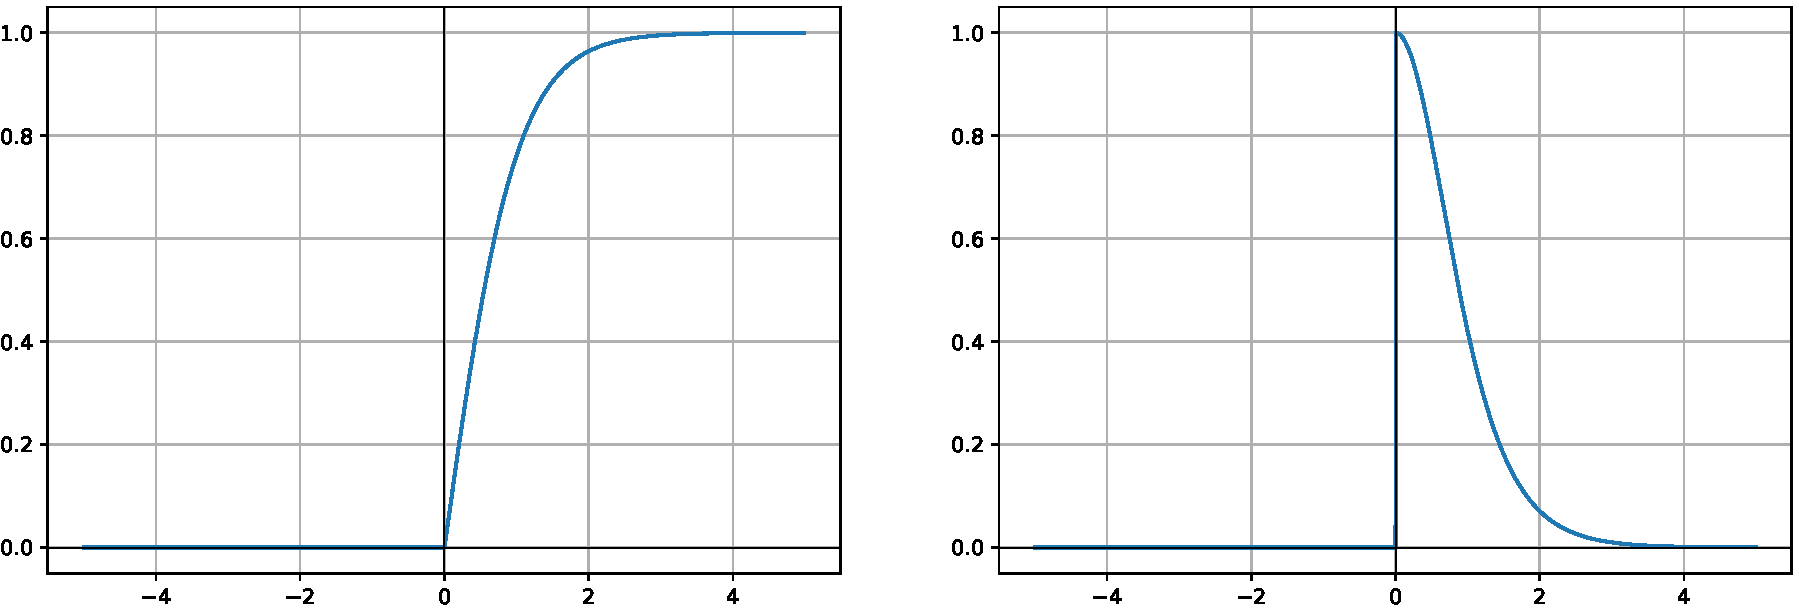
\includegraphics[width=\textwidth]{Rectified_tanh.pdf}
\centering
\caption{Ispravljeni tanh i njegova derivacija}
\label{fig:rectified_tanh}
\end{figure}

\begin{equation}
\label{eq:rectanh}
???
\end{equation}

\todo{koji problem rješava}
\todo{svojstva}
\todo{problemi}

\subsection{Softmax}

\todoimg{}

\begin{equation}
\label{eq:softmax}
\begin{split}
f(\vec{x}) = \frac{e^{\vec{x}}}{\sum_ie^{\vec{x_i}}}
\end{split}
\qquad
\begin{split}
f'(x) = \frac{e^x}{1+e^x}
\end{split}
\end{equation}

\todo{koji problem rješava}
\todo{svojstva}
\todo{problemi}

\iffalse %%%%%%%%%%%%%%%%%%%%%%%%%%%%%%%%%%%%%%%%%%%%%%%%%%%%%%%%%%%%%%%%%%%%%%%%%%%%%%%
\subsection{Maxout}

\todoimg{}

\begin{equation}
???
\end{equation}

\todo{koji problem rješava}
\todo{svojstva}
\todo{problemi}
\fi %%%%%%%%%%%%%%%%%%%%%%%%%%%%%%%%%%%%%%%%%%%%%%%%%%%%%%%%%%%%%%%%%%%%%%%%%%%%%%%%%%%%

\subsection{Softsign}

\begin{figure}[H]
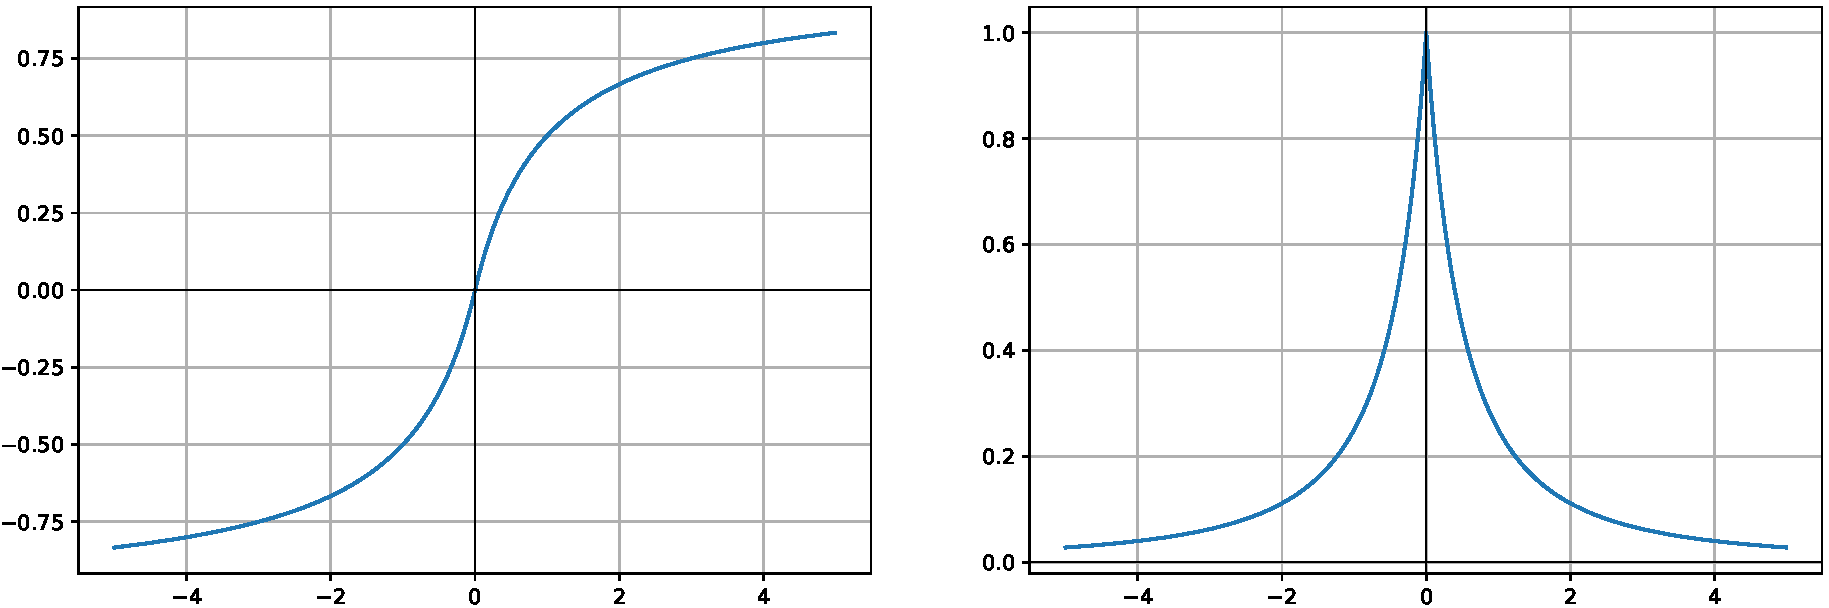
\includegraphics[width=\textwidth]{Softsign.pdf}
\centering
\caption{Softsign i njegova derivacija}
\label{fig:softsign}
\end{figure}

\begin{equation}
\label{eq:softsign}
\begin{split}
f(x) = \frac{x}{1+|x|}
\end{split}
\qquad
\begin{split}
f'(x) = \frac{1 + |x| - x \cdot sign(x)}{(1+|x|)^2}
\end{split}
\end{equation}

\todo{koji problem rješava}
\todo{svojstva}
\todo{problemi}

\subsection{Sinus (sin)}

\begin{figure}[H]
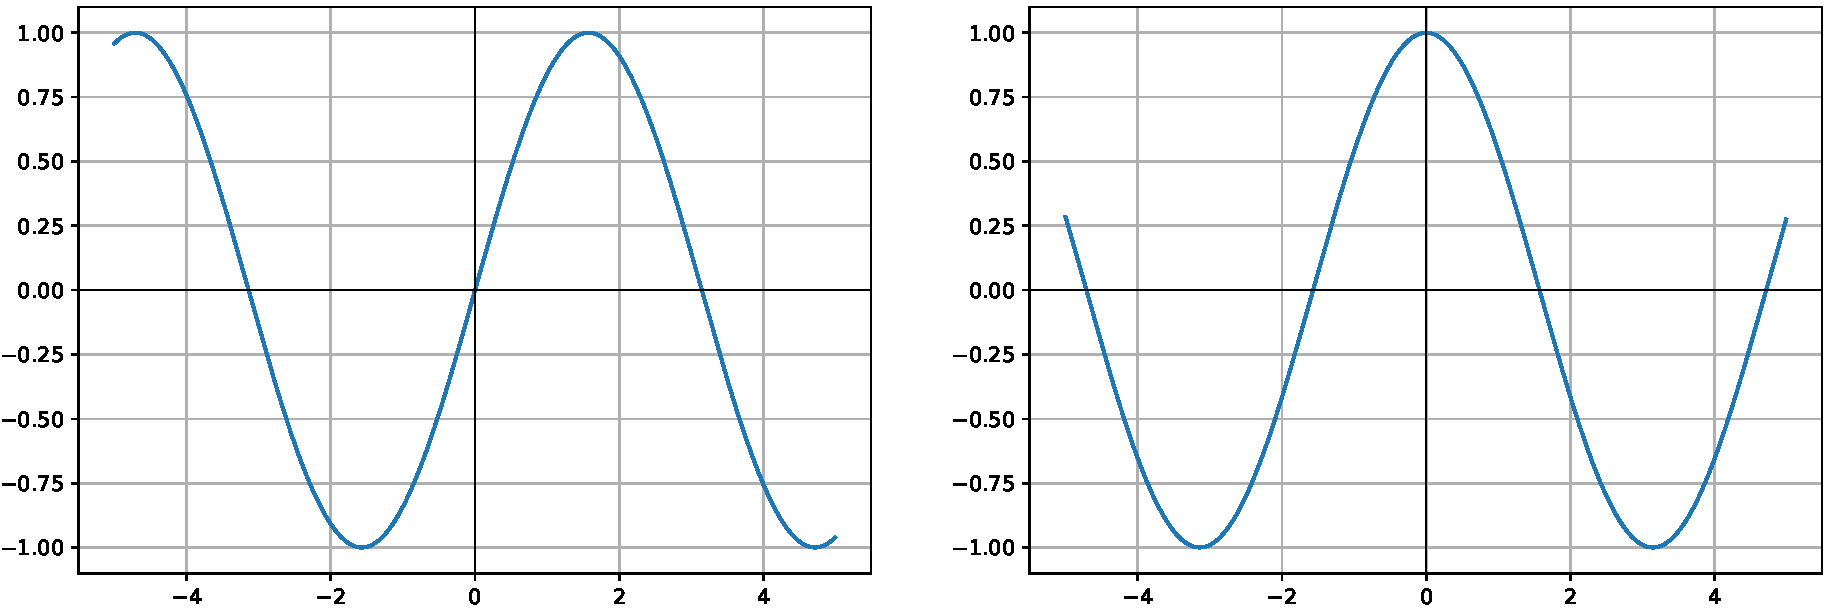
\includegraphics[width=\textwidth]{Sin.pdf}
\centering
\caption{Sinusoida i njegova derivacija}
\label{fig:sin}
\end{figure}

\begin{equation}
\label{eq:sin}
\begin{split}
f(x) = sin(x)
\end{split}
\qquad
\begin{split}
f'(x) = cos(x)
\end{split}
\end{equation}

%Sinus je periodička funkcija te nema teorijsku podlogu za uporabu u neuronskim mrežama, za razliku od monotonih funkcija.
%\todo{članak dokaz univerzalne aproksimacije monotonih fja}

Sinusoida se često pojavljuje u radovima pretrage aktivacijskih funkcija \citep{elish} pa tako i u ovom radu te pokazuje obećavajuće rezultate. U radu \citet{taming_waves} autori predstavljaju problematiku učenja sa sinusoidom na jednostavnom problemu. Problem stvaraju brojni lokalni optimumi na koje je izrazito osjetljiv gradijentni spust. Problem je ublažava učenje stohastičkim gradijentnim spustom koji zaglađuje valovitost funkcije gubitka. Dodatno, autori pokazuju da neuronska mreža zapravo ne ovisi snažno o periodičnosti funkcije tako da su rezultate usporedili s ograničenom sinusoidom \eqref{eq:trsin}. Članak nije prošao postupak recenzije jer su dodatni eksperimenti urodili nekonzistentnim rezultatima u usporedbi s tangensom hiperbolnim.

Po uzoru na slične funkcije kao što je sigmoida \figref{fig:sigmoid} i tangens hiperbolni \figref{fig:tanh}, sinusoida najveću vrijednost gradijenta daje upravo kada je aktivacija jednaka 0 (u ograničenom intervalu).

\subsection{Ograničeni sinus (TrSin)}
\label{func:trsin}
\engl{Truncated sine}

\begin{figure}[H]
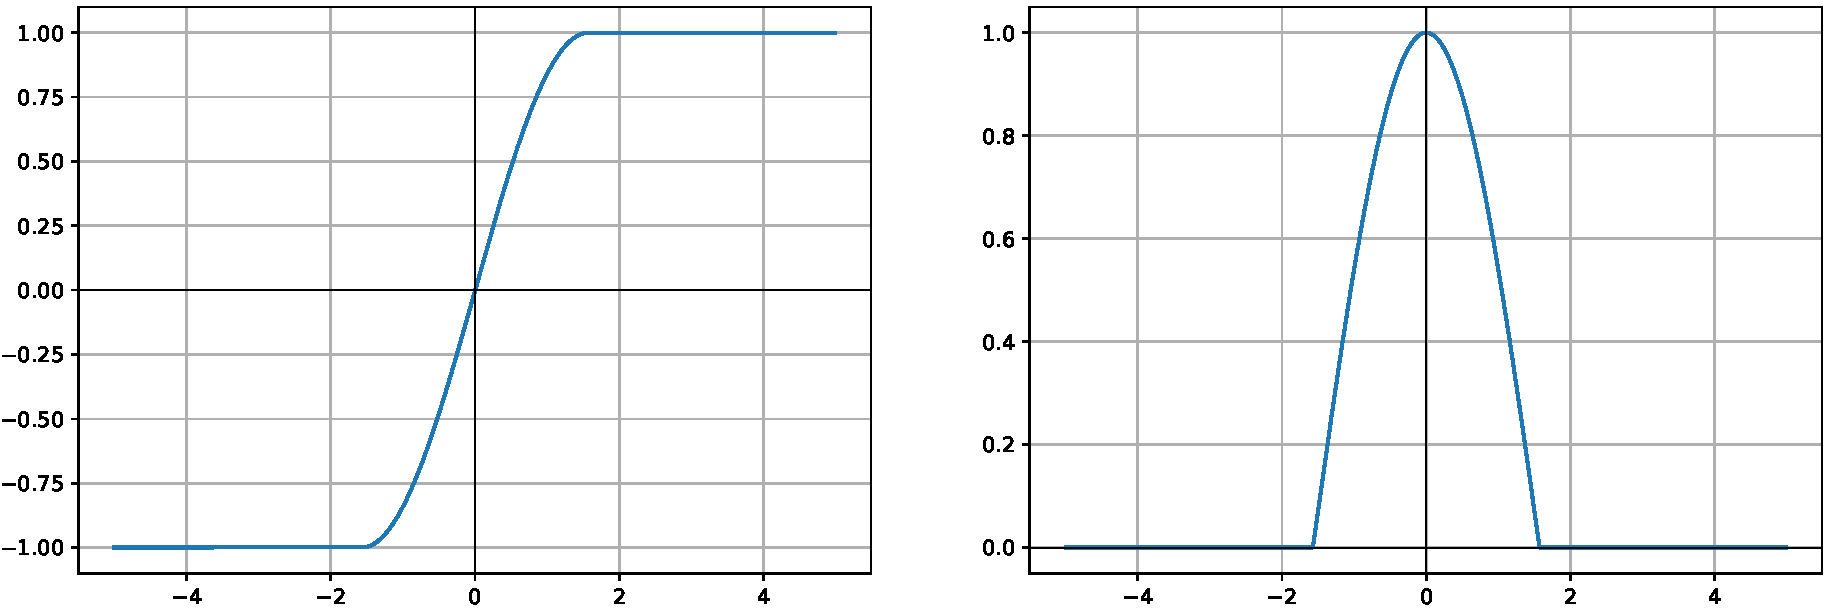
\includegraphics[width=\textwidth]{TrSin.pdf}
\centering
\caption{Ograničeni sinus i njegova derivacija}
\label{fig:trsin}
\end{figure}

\begin{equation}
\label{eq:trsin}
\begin{split}
f(x) =
\begin{cases}
0, \quad x < \frac{\pi}{2} \\
sin(x), \quad |x| \leq \frac{\pi}{2} \\
1, \quad \otherwise
\end{cases}
\end{split}
\qquad
\begin{split}
f'(x) =
\begin{cases}
cos(x), \quad |x| \leq \frac{\pi}{2} \\
0, \quad \otherwise
\end{cases}
\end{split}
\end{equation}

Ograničeni sinus korišten je u radu \citet{taming_waves} za usporedbu s klasičnom sinusoidom i tangensom hiperbolnim. U usporedbi sa sinusom ispituje se utjecaj periodičnosti sinusa na performanse. S tangensom hiperbolnim uspoređene su performanse zbog sličnosti u obliku krivulja.

\subsection{Kosinus (cos)}

\begin{figure}[H]
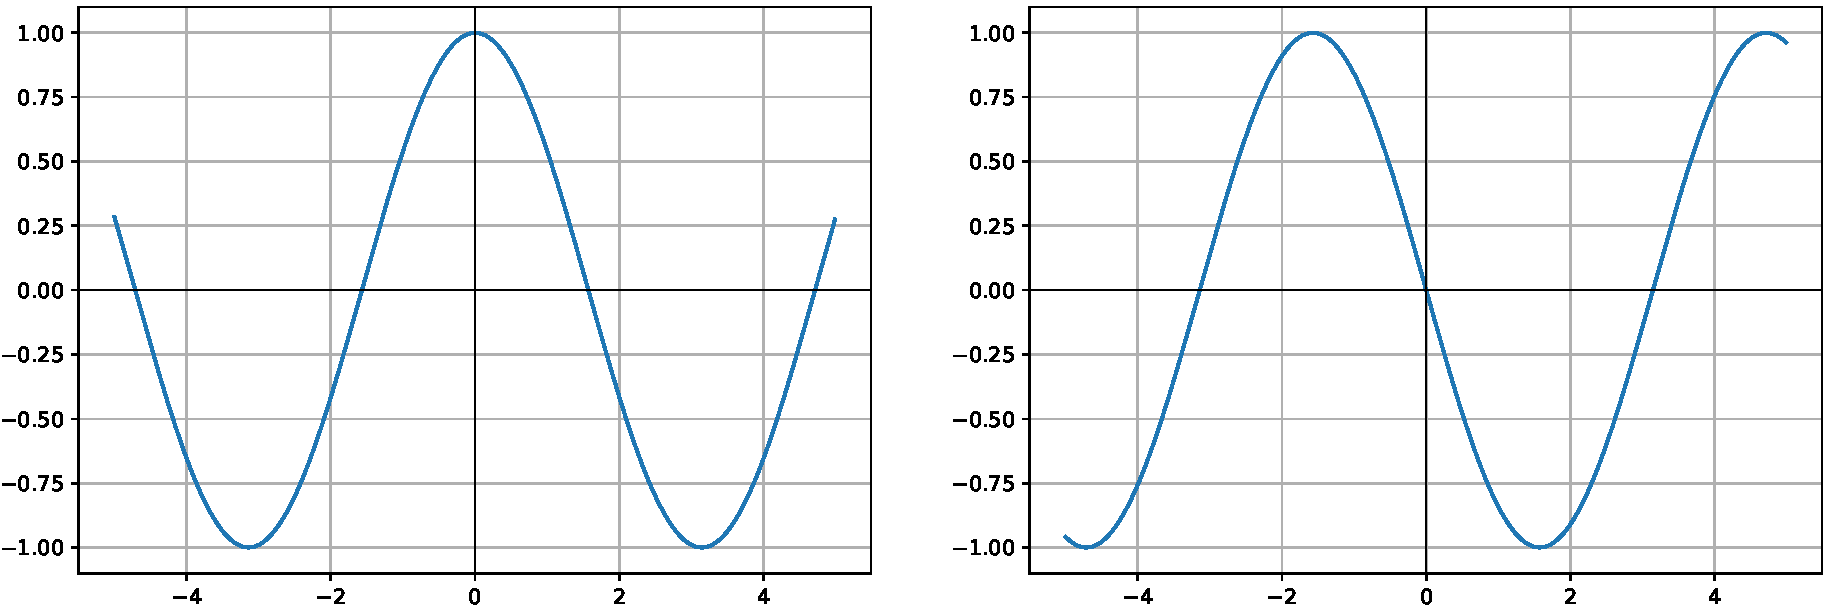
\includegraphics[width=\textwidth]{Cos.pdf}
\centering
\caption{Kosinus i njegova derivacija}
\label{fig:cos}
\end{figure}

\begin{equation}
\label{eq:cos}
\begin{split}
f(x) = cos(x)
\end{split}
\qquad
\begin{split}
f'(x) = -sin(x)
\end{split}
\end{equation}

Kosinus je funkcija sinusa pomaknuta za četvrtinu periode te dijeli ista svojstva i probleme. no, s obzirom da je pomak relativno velik u odnosu na očekivane veličine ulaza, može se promatrati kao zasebna aktivacijska funkcija. Derivacija kosinusa se poprilično razlikuje od ostalih aktivacijskih funkcija. Unatoč tome, daje vrlo kompetitivne rezultate \secref{sec:rezultati}.
\begin{equation}
cos(x) = sin(x + \frac{\pi}{2}) \approx sin(x + 1.571)
\end{equation}

\iffalse %%%%%%%%%%%%%%%%%%%%%%%%%%%%%%%%%%%%%%%%%%%%%%%%%%%%%%%%%%%%%%%%%%%%%%%%%%%%%%%
\subsection{Ograničeni kosinus (TrCos)}
\engl{Truncated cosine}

\begin{figure}[H]
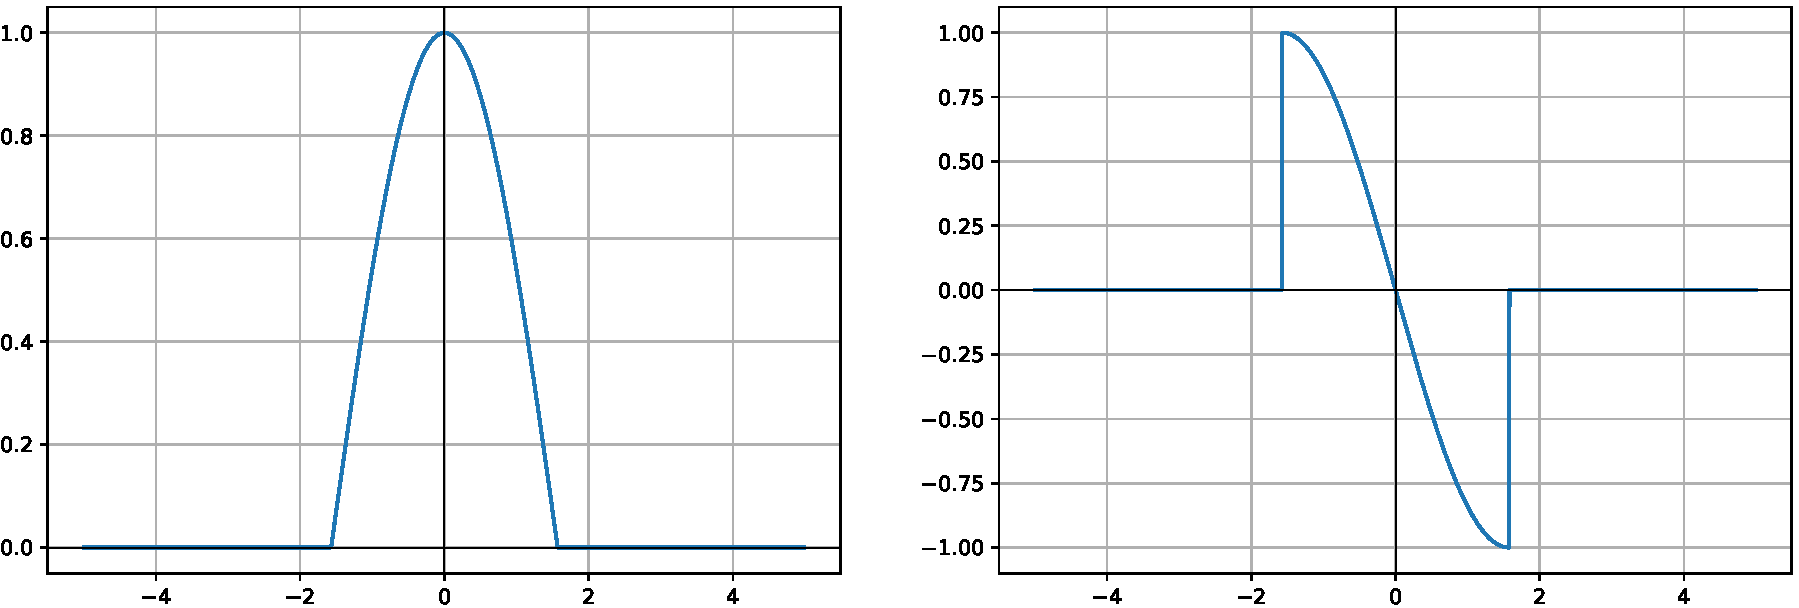
\includegraphics[width=\textwidth]{TrCos.pdf}
\centering
\caption{Ograničeni kosinus i njegova derivacija}
\end{figure}

\begin{equation}
\begin{split}
f(x) =
\begin{cases}
cos(x), \quad |x| \leq \frac{\pi}{2} \\
0, \quad \otherwise
\end{cases}
\end{split}
\qquad
\begin{split}
f'(x) =
\begin{cases}
-sin(x), \quad |x| \leq \frac{\pi}{2} \\
0, \quad \otherwise
\end{cases}
\end{split}
\end{equation}

Ograničeni kosinus autori nisu pronašli u literaturi, no navodi se zbog potrebe ispitivanja ovisnosti o periodičnosti kosinusa (po uzoru na poglavlje \ref{func:trsin}).
\fi %%%%%%%%%%%%%%%%%%%%%%%%%%%%%%%%%%%%%%%%%%%%%%%%%%%%%%%%%%%%%%%%%%%%%%%%%%%%%%%%%%%%

\subsection{Parabola $x^2$}

\begin{figure}[H]
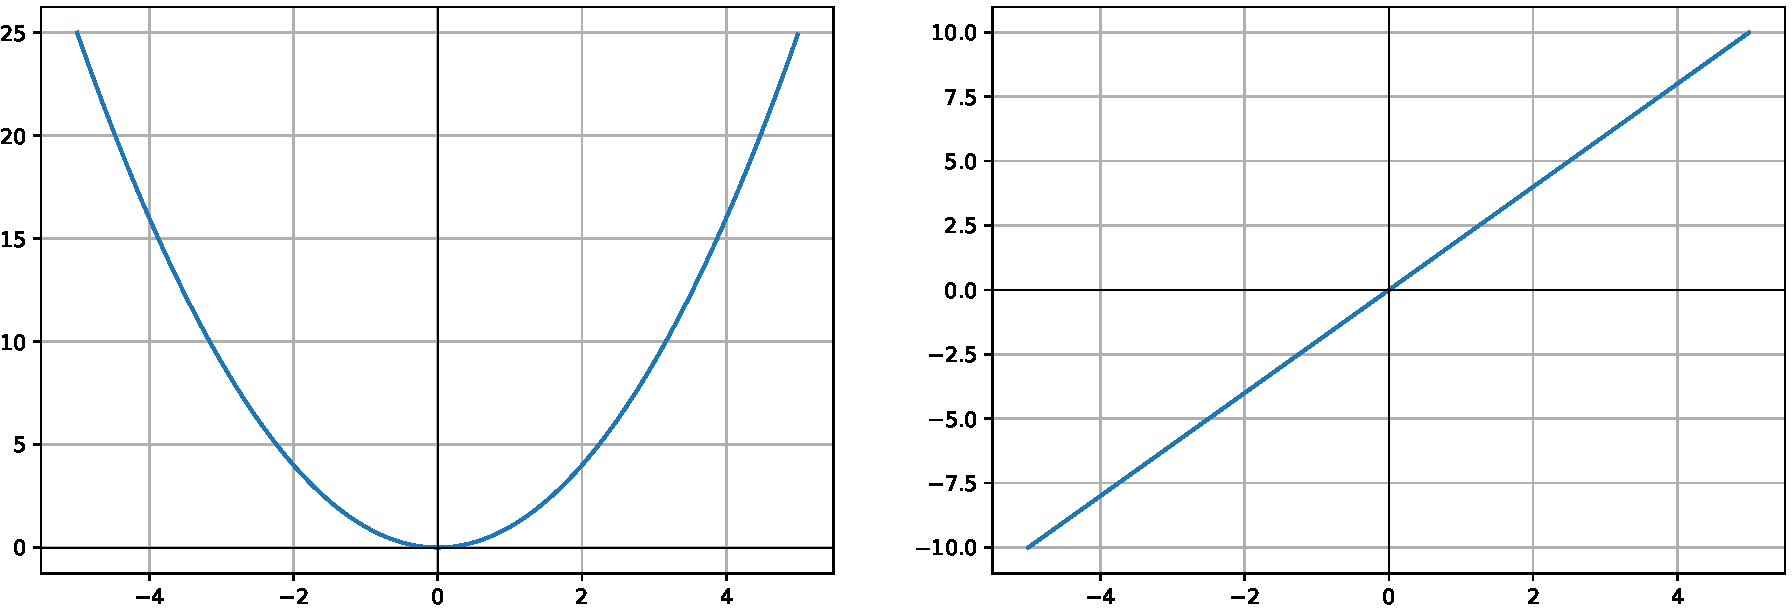
\includegraphics[width=\textwidth]{Pow2.pdf}
\centering
\caption{Parabola i njena derivacija}
\end{figure}

\begin{equation}
\begin{split}
f(x) = x^2
\end{split}
\qquad
\begin{split}
f'(x) = 2x
\end{split}
\end{equation}

\todo{koji problem rješava}
\todo{svojstva}
\todo{problemi}

\iffalse %%%%%%%%%%%%%%%%%%%%%%%%%%%%%%%%%%%%%%%%%%%%%%%%%%%%%%%%%%%%%%%%%%%%%%%%%%%%%%%
\subsection{Kubna parabola $x^3$}

\begin{figure}[H]
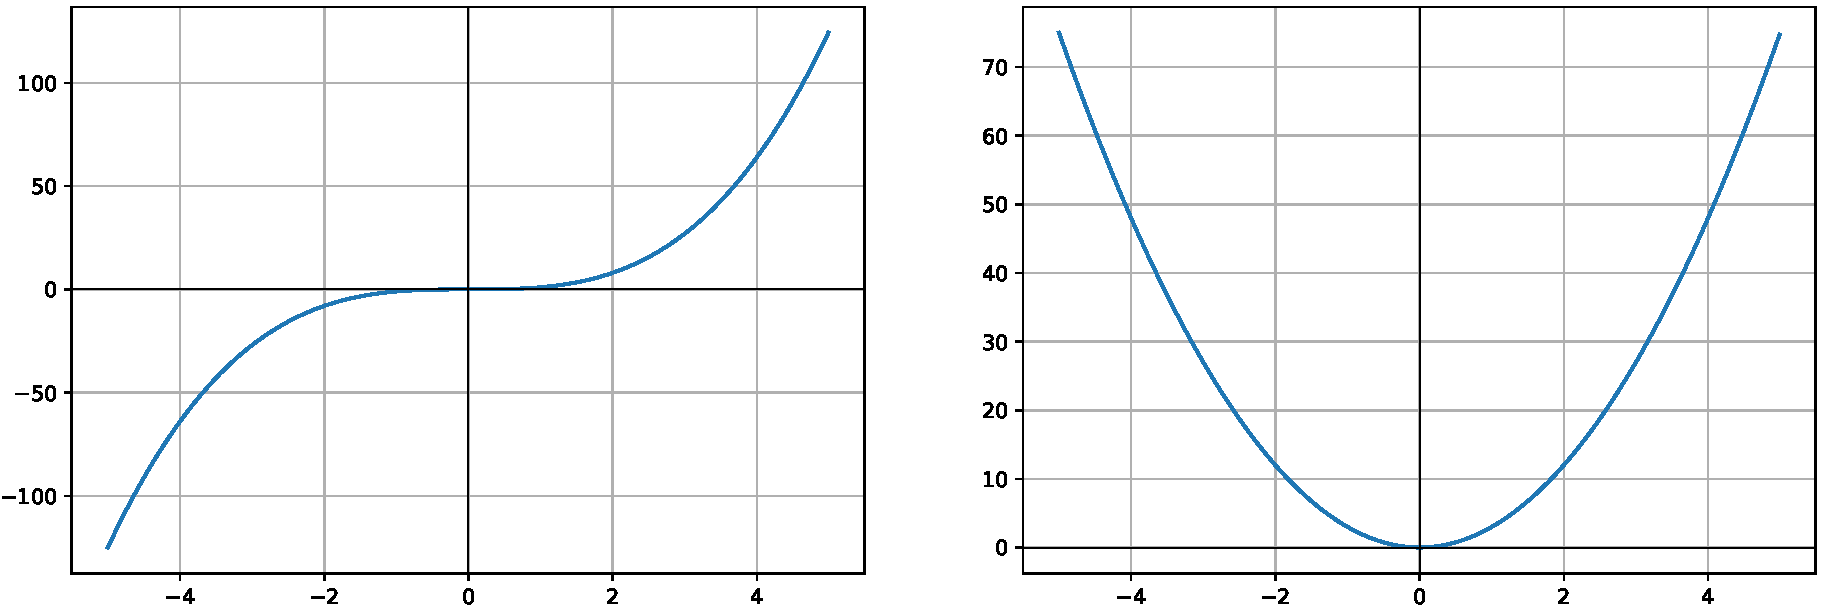
\includegraphics[width=\textwidth]{Pow3.pdf}
\centering
\caption{Kubna parabola i njena derivacija}
\end{figure}

\begin{equation}
\begin{split}
f(x) = x^3
\end{split}
\qquad
\begin{split}
f'(x) = 3x^2
\end{split}
\end{equation}

\todo{koji problem rješava}
\todo{svojstva}
\todo{problemi}
\fi %%%%%%%%%%%%%%%%%%%%%%%%%%%%%%%%%%%%%%%%%%%%%%%%%%%%%%%%%%%%%%%%%%%%%%%%%%%%%%%%%%%%

\subsection{Gaussova krivulja bez normalizacije}

\begin{figure}[H]
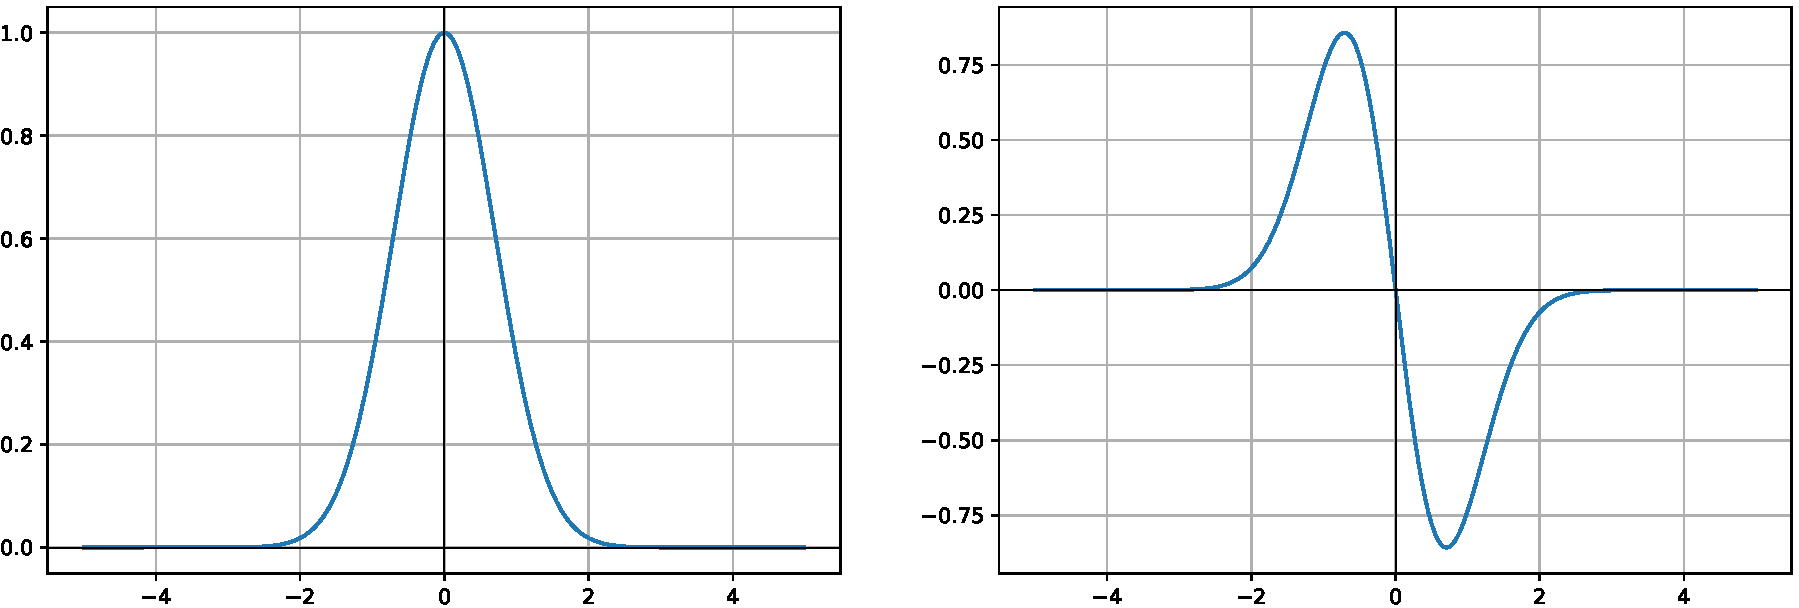
\includegraphics[width=\textwidth]{Gauss.pdf}
\centering
\caption{Gaussova krivulja bez normalizacije i njena derivacija}
\label{fig:gauss}
\end{figure}

\begin{equation}
\label{eq:gauss}
\begin{split}
f(x) = e^{-x^2}
\end{split}
\qquad
\begin{split}
f'(x) = -2x \cdot f(x)
\end{split}
\end{equation}

\todo{koji problem rješava}
\todo{svojstva}
\todo{problemi}

\iffalse %%%%%%%%%%%%%%%%%%%%%%%%%%%%%%%%%%%%%%%%%%%%%%%%%%%%%%%%%%%%%%%%%%%%%%%%%%%%%%%
\section{Adaptivne aktivacijske funkcije}
U nastavku su navedene adaptivne aktivacijske funkcije koje je autor pronašao u literaturi. Funkcije su adaptivne jer sadrže parametre koje je moguće optimizirati. Njihov izlaz ovisi o ulazu u funkciju i adaptivnim parametrima. Za svaku funkciju napisana je formula i iscrtan izgled funkcije i njene derivacije te navedena neka poznata svojstva.

\subsection{Parametrizirana ispravljena linearna jedinica (PReLU)}
\engl{Parametric ReLU}

\todoimg{}

\begin{equation}
\begin{split}
f(x) &= \begin{cases}
x,			& \text{ako } x > 0 \\
\alpha x,	& \otherwise
\end{cases} \\
&= max(\alpha x, x)
\end{split}
\qquad
\begin{split}
f'(x) = 
\begin{cases}
1,		& \text{ako } x > 0 \\
\alpha,	& \otherwise
\end{cases}
\end{split}
\end{equation}
\begin{equation*}
\alpha \text{ je učeći parametar}
\end{equation*}

\todo{koji problem rješava}
\todo{svojstva}
\todo{problemi}

\subsection{Adaptivna razlomljena linearna funkcija (APL)}
\engl{Adaptive piecewise linear}

\todoimg{}

\begin{equation}
\begin{split}
f(x) &=  \\
\end{split}
\qquad
\begin{split}
f'(x) = 
\end{split}
\end{equation}
\begin{equation*}
\alpha \text{ je učeći parametar}
\end{equation*}

\todo{koji problem rješava}
\todo{svojstva}
\todo{problemi}

\subsection{ReLU oblika S (S-ReLU)}
\engl{S-shaped ReLU}

\begin{figure}[H]
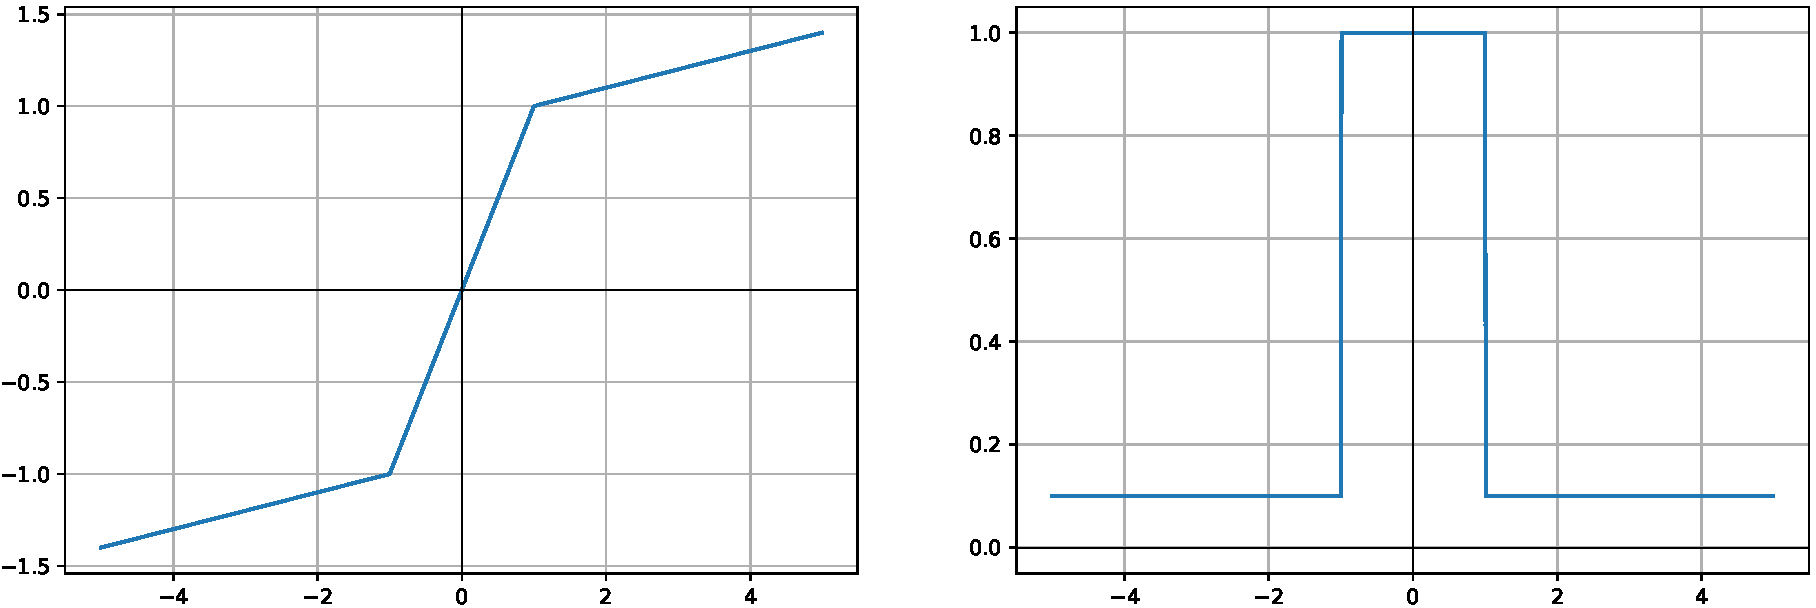
\includegraphics[width=\textwidth]{PLU.pdf}
\centering
\caption{Funkcija PLU i njena derivacija}
\end{figure}

\begin{equation}
\begin{split}
f(x) &=
\begin{cases}
x, \quad |x| \leq c \\
\alpha \cdot x, \quad \otherwise
\end{cases} \\
&= \max(\alpha x - c(1-\alpha), \min(x, \alpha x + c (1-\alpha)))
\end{split}
\quad
\begin{split}
f'(x) =
\begin{cases}
1, \quad |x| \leq c \\
\alpha, \quad \otherwise
\end{cases}
\end{split}
\end{equation}
\begin{equation*}
\alpha, c \in \realnum
\end{equation*}

\todo{koji problem rješava}
\todo{svojstva}
\todo{problemi}

\section{Aktivacijske funkcije posebne namjene}
U nastavku su navedene aktivacijske funkcije posebne namjene koje je autor pronašao u literaturi. Navedene funkcije uvedene su za pospješivanje neuronskih mreža specifičnih arhitektura. Funkcije nisu korištene u ovom radu, no autor smatra da ih je dobro spomenuti. Za svaku funkciju napisana je formula i iscrtan izgled funkcije i njene derivacije te navedena neka poznata svojstva.

\subsection{(DReLU)}
\engl{Dual ReLU}

\todoimg{}

\begin{equation}
???
\end{equation}

\todo{koji problem rješava}
\todo{svojstva}
\todo{problemi}

Koristi se u rekurzivnim neuronskim mrežama kako bi se ... LSTM

\subsection{Hijerarhijski softmax}
\engl{hierarchical softmax}

\todoimg{}

\begin{equation}
???
\end{equation}

\todo{koji problem rješava}
\todo{svojstva}
\todo{problemi}
\fi %%%%%%%%%%%%%%%%%%%%%%%%%%%%%%%%%%%%%%%%%%%%%%%%%%%%%%%%%%%%%%%%%%%%%%%%%%%%%%%%%%%%

%--------------------------------------------------------------------------------------%
\chapter{Optimizacija aktivacijske funkcije genetskim programiranjem}

\section{Genetsko programiranje}
Genetsko programiranje je područje evolucijskog računarstva koje se bavi algoritmima pretrage hijerarhijskih struktura. Razlikuje se od susjednih područja po tome što je genotip izvršivi program i dobrota jedinke se dobiva njenim izvršavanjem. Genotip tipično poprima stablastu strukturu te u pravilu nema zadanu veličinu, no može se ograničiti. Dijelovi genotipa definirani su jezikom, skupom funkcija i listova koje definiraju prostor pretraživanja. U ovom radu se elementi jezika nazivaju čvorovima. Jezik mora biti zatvoren (izlaz svakog čvora je kompatibilan s ulazom svakog drugog čvora) i dovoljan (rješenje je moguće predstaviti isključivo koristeći elemente jezika). \citep{comp_intelligence}

Evolucijski algoritmi su intrinzično stohastični te omogućuju globalno i lokalno pretraživanje prostora, za razliku od gradijentnog spusta koji lokalno pretražuje prostor. Dok se lokalnim pretraživanjem pretražuje usko susjedstvo oko točke u prostoru, globalno pretraživanje pretražuje točke po čitavoj domeni unutar dosega. To svojstvo osigurava otpornost evolucijskih algoritama na prepreke koje ograničavaju gradijentni spust \secref{sec:gradijentni_spust}. Opseg pretrage određen je jezikom te ograničenjima pri inicijalizaciji populacije i operatorima pretrage. Treba razlikovati genotipski i fenotipski prostor. Genotipski prostor definiran je jezikom i najvećom dubinom stabla, dok je fenotipski prostor definiran dekoderom koji genotip pretvara u primjenjivo rješenje. Iako ograničenja u genotipu ograničavaju fenotip, mogu imati nepredvidiv utjecaj.

\subsection{Građa}
Kao i ostali evolucijski algoritmi, algoritam genetskog programiranja sastoji se od više elemenata koji definiraju način pretrage. \textbf{Inicijalizator populacije} služi stvaranju početnih točaka iz kojih kreće pretraga i poželjno je da stvara što raznolikija rješenja (globalna pretraga). \textbf{Operator odabira} iz populacije uzima po jedan par jedinki za roditelje i jednu ili dvije jedinke za zamjenu. Pri RouletteWheel odabiru vjerojatnosti odabira jedinki proporcionalna je njihovoj dobroti. Pri turnirskom odabiru nasumično se odabire $n$ jedinki, dvije najbolje postaju roditeljima te ona najlošija biva odabrana za zamjenu. Operatori odabira naginju zadržavanju dobrih genotipa u populaciji i time osiguravaju konvergenciju algoritma (lokalna pretraga). \textbf{Operator križanja} iz genotipa odabranih roditelja izgradi jedno ili dva djeteta koja će biti dio nove populacije. Operatori križanja miješaju genotipove jedinki zadržavajući svojstva dobrih i time pomažu konvergenciji algoritma (lokalna pretraga). \textbf{Operator mutacije} nad stvorenim djetetom unosi nasumičnu izmjenu i time osigurava unos novih informacija u populaciji (globalna pretraga). Često se definira po nekoliko različitih operatora križanja i mutacije koji različito djeluju na pretragu te se time upravlja globalnošću pretrage. Pristup izgradnji nove populacije na temelju stare utječe na snagu konvergencije algoritma. \textbf{Generacijski pristup} će u svakoj iteraciji čitavu populaciju zamijeniti djecom. Pri tome često se koristi \textbf{elitizam} kojim se garantira očuvanje najbolje jedinke iz stare u novu populaciju. \textbf{Eliminacijski pristup} definira postotak populacije koji će biti zamijenjen djecom.
\newline
\newline
\begin{algorithm}[H]
\DontPrintSemicolon
\KwIn{funkcija $f(x)$}
\KwIn{kriterij zaustavljanja $K$}
\KwIn{veličina populacije $N$}
$InicijalizirajPopulaciju(populacija, N)$ \;
\While{$K$ nije zadovoljen}{
$x^* \gets OdaberiNajbolju(x, populacija)$ \;
definiraj novu populaciju: $populacija'$ \;
\For{$N$ puta}{
$(p_1, p_2) \gets OdaberiRoditelje(populacija)$ \;
$c \gets OperatorKrižanja(p_1, p_2)$ \;
$OperatorMutacije(c)$ \;
$DodajPopulaciji(c, populacija')$
}
$populacija \gets populacija'$
}
\KwResult{pronađena optimalna jedinka $x^*$}
\;
\caption{Tipičan generacijski evolucijski algoritam}
\label{alg:ea}
\end{algorithm}

\paragraph{}
Evolucijski algoritmi podržavaju nekoliko glavnih hiperparametara. \textbf{Veličina populacije} definira broj istovremenih točaka u prostoru te o njoj ovisi vjerojatnost pronalaska optimuma. Operatori mutacije unose izmjene u genomu i njihova primjena se regulira \textbf{vjerojatnošću primjene}. \textbf{Kriteriji zaustavljanja} određuju završetak pretrage i mogu ovisiti o kvaliteti rješenja ili raspoloživim resursima. \textbf{Broj iteracija} analogan je onome u gradijentnom spustu \secref{sec:gradijentni_spust} i često se koristi kao gornja granica za vremenski trošak izvođenja. \textbf{Broj evaluacija} je koristan kada je poznato trajanje pojedine evaluacije želi se sukladno raspoloživom vremenu odrediti veličina populacije. \textbf{Raspoloživo vrijeme} se koristi kao i broj iteracija, ali u situacijama kada nije poznato trajanje pojedine iteracije algoritma. \textbf{Kvaliteta rješenja} je koristan kriterij zaustavljanja ako postoji definirana granica zadovoljavajuće kvalitete. Razne inačice evolucijskih algoritama mogu uvesti brojne dodatne hiperparametre.

\iffalse %%%%%%%%%%%%%%%%%%%%%%%%%%%%%%%%%%%%%%%%%%%%%%%%%%%%%%%%%%%%%%%%%%%%%%%%%%%%%%%%%%%%%%%%%%
\subsection{Simbolička regresija}
Simbolička regresija je postupak izgradnje funkcije koja dobro aproksimira uzorke stvarne funkcije.
\fi %%%%%%%%%%%%%%%%%%%%%%%%%%%%%%%%%%%%%%%%%%%%%%%%%%%%%%%%%%%%%%%%%%%%%%%%%%%%%%%%%%%%%%%%%%%%%%%

\subsection{Neuroevolucija genetskim programiranjem}
Proizvoljnu neuronsku mrežu moguće je predstaviti stablom, gdje su čvorovi mreže ulazne i aktivacijske funkcije neurona te dodatne operacije (normalizacija grupe, dropout i ostali). Takav pristup korišten je u \citet{evo_atari} algoritmom kartezijevog genetskog programiranja. Metoda NEAT dijeli graf na neurone i težine istovremeno pretražuje prostor arhitektura i težina \citep{neat}. Postoje i metode indirektne evolucije arhitekture neuronskih mreža čiji genotip je potrebno dekodirati. Takve metode smanjuju prostor pretraživanja i time efikasno istražuju vrlo složene arhitekture \citep{gruau}.

\iffalse %%%%%%%%%%%%%%%%%%%%%%%%%%%%%%%%%%%%%%%%%%%%%%%%%%%%%%%%%%%%%%%%%%%%%%%%%%%%%%%%%%%%%%%%%%
\todo{negdje spomeni da su neuralke zapravo vrlo ograničene jer se ograničava prostor mogućnosti zadavanjem fiksnih aktivacijskih fja, arhitekture i načina optimizacije (induktivna pristranost ograničavanjem skupa hipoteza). leži negdje između GP i ručno izgrađenih modela (jer je neuralka samo stablo funkcija kao u TF). CGP unosi ograničenje strukture što je bliže neuralki i daje zanimljive rezultate (atari cgp). Čini se da im godi balans između strukture i nasumičnosti.}
\fi %%%%%%%%%%%%%%%%%%%%%%%%%%%%%%%%%%%%%%%%%%%%%%%%%%%%%%%%%%%%%%%%%%%%%%%%%%%%%%%%%%%%%%%%%%%%%%%%

\section{Optimizacija aktivacijskih funkcija}
U literaturi postoje brojni radovi na temu optimizacija aktivacijskih funkcija, neki od kojih se služe genetskim programiranjem. U nastavku su detaljnije objašnjeni radovi koje je autor pronašao na temu optimizacije aktivacijskih funkcija.

U radu \citet{swish} autori smanjuju prostor pretraživanja definirajući strukturu funkcija koje se pretražuju u obliku bloka. Blokove definiraju kompozicijom binarne i dviju unarnih funkcija te istražuju rekurzivna proširenja istog bloka (umjesto jedne unarne funkcije ponavlja se blok). Rekurzivna mreža predviđa funkciju na idućem mjestu u bloku temeljem prethodno odabrane funkcije. Izgrađeni blok koristi se kao aktivacijska funkcija dubokih mreža te se postignuta točnost uzima kao vrijednost nagrade za optimizaciju potpornim učenjem. Rezultat pretrage je funkcija $Swish$ \secref{func:swish} koja konzistentno nadjačava $ReLU$ \secref{func:relu} i ostale popularne funkcije.

U radu \citet{elish} autori koriste hibridni genetski algoritam kako bi evoluirali funkciju različito definiranu na pozitivnoj i negativnoj domeni. Dijelovi funkcije su predstavljeni stablima i križaju ih posebnim operatorima koji odvojeno mijenjaju pozitivnu i negativnu stranu. Skup čvorova su osnovne aritmetičke operacije, a listovi su popularne aktivacijske funkcije bez konstanti. Autori predstavljaju i nove aktivacijske funkcije (poglavlja \ref{func:elish}, \ref{func:hard_elish}) koje su ručno izgradili s ciljem kombiniranja dobrih svojstava manjih funkcija. Na tri podatkovna skupa pokazuju da su njihove funkcije najbolje.

Rad \citet{cube_spline_func} predstavlja aktivacijsku funkciju definiranu kubnim splajnom. Koristi se genetski algoritam za pronalazak točaka kojima se interpolira aktivacijska funkcija te pronalazak arhitekture čitave mreže. Rezultati pokazuju da pronađene funkcije ostvaruju poboljšanje nad sigmoidom na zadatcima klasifikacije.

\section{Genetsko programiranje s taboo listom}
Klasičan algoritam genetskog programiranja često dovodi do stvaranja identičnih jedinki u populaciji što loše utječe na globalnost pretrage. Stoga se u ovom radu unosi primjena taboo liste u proces algoritma. Nakon stvaranja djeteta klasičnim koracima (križanje i mutacija) dodaje se dodatan korak u kome se dijete mutira dok ne postane jedinstveno. Kako algoritam ne bi zapeo definira se gornja granica dozvoljenog broja mutacija. Kada je stvoreno jedinstveno dijete, ono se dodaje u populaciju i zabilježi na kraj taboo liste.
\newline
\newline
\begin{algorithm}[H]
\DontPrintSemicolon
\KwIn{funkcija $f(x)$}
\KwIn{kriterij zaustavljanja $K$}
\KwIn{veličina populacije $N$}
\KwIn{veličina taboo liste $T$}
$InicijalizirajPopulaciju(populacija, N)$ \;
$taboo \gets StvoriPraznuTabooListu(T)$ \;
\While{$K$ nije zadovoljen}{
$x^* \gets OdaberiNajbolju(x, populacija)$ \;
definiraj novu populaciju: $populacija'$ \;
\For{$N$ puta}{
$(p_1, p_2) \gets OdaberiRoditelje(populacija)$ \;
$c \gets OperatorKrižanja(p_1, p_2)$ \;
$OperatorMutacije(c)$ \;
\While{$x \in taboo$}{
	$OperatorMutacije(c)$
}
$DodajNaKraj(c, taboo)$ \;
\If{$|taboo| > T$}{
	$UkloniPrvog(taboo)$
}
$DodajPopulaciji(c, populacija')$
}
$populacija \gets populacija'$
}
\KwResult{pronađena optimalna jedinka $x^*$}
\;
\caption{Genetsko programiranje s taboo listom}
\label{alg:gp_taboo}
\end{algorithm}

Veličina taboo liste definira koliko se često smije pojaviti već postojeća jedinka u populaciji. U ovom radu se istražuje utjecaj na razini broja iteracija. Na primjer, ako je populacija veličine $10$ jedinki tada će veličina taboo liste za $2$ iteracije biti veličine $20$. Za vrijednost $0$ algoritam se ponaša identično klasičnom algoritmu genetskog programiranja.

Zbog ponovljenog mutiranja jedinke treba paziti na balans između mutacija koje povećavaju ili smanjuju dubinu stabla. U suprotnom će jedinke vrlo brzo postati vrlo velike što je nepoželjno za pretraživanje aktivacijskih funkcija \citep{swish} ili će ostati suviše male što ograničava pretraživanje šireg prostora.

\subsection{Skup čvorova (prostor pretraživanja)}
\label{sec:node_set}
Skup čvorova koji se koriste pri pretraživanju definiraju prostor pretraživanja. Skup čvorova je implementiran tako da razlikuje čvorove različitih stupnjeva i omogućuje operatorima selektivni, nasumično selektivni ili potpuno nasumičan pristup. Početna vrijednost konstante pri dohvatu je postojana i definira se unaprijed, a vrijednost pojedine konstante u stablima mijenja se operatorima.

\begin{table}[H]
\centering
\begin{tabular}[t]{lr}
\begin{tabular}[t]{l|c|r}
\textbf{Naziv} & \textbf{Funkcija} & \textbf{Stupanj} \\
\hline
x		& $x$					& 0 \\
const	& $c \in \realnum$		& 0 \\
\hline
+		& $x + y$				& 2 \\
-		& $x - y$				& 2 \\
*		& $x \cdot y$			& 2 \\
/		& $\frac{x}{y + 10^{-12}}$	& 2 \\
\hline
min		& $min(x, y)$			& 2 \\
max		& $max(x, y)$			& 2 \\
abs		& $|x|$					& 1 \\
\hline
sin		& $sin(x)$				& 1 \\
cos		& $cos(x)$				& 1 \\
tan		& $tan(x)$				& 1 \\
\hline
exp		& $e^x$					& 1 \\
log		& $log_e(x)$				& 1 \\
pow2		& $x^2$					& 1 \\
pow3		& $x^3$					& 1 \\
pow		& $x^y$					& 2 \\
\end{tabular}
& \quad
\begin{tabular}[t]{l|c|r}
\textbf{Naziv} & \textbf{Funkcija} & \textbf{Stupanj} \\
\hline
relu		& \eqref{eq:relu}		& 1 \\
lrelu	& \eqref{eq:lrelu}		& 1 \\
threlu 	& \eqref{eq:threlu}		& 1 \\
sotplus	& \eqref{eq:softplus}	& 1 \\
elu		& \eqref{eq:elu}			& 1 \\
selu		& \eqref{eq:selu}		& 1 \\
swish	& \eqref{eq:swish}		& 1 \\
sigmoid	& \eqref{eq:sigmoid}		& 1 \\
hsigmoid & \eqref{eq:hsigmoid}	& 1 \\
tanh		& \eqref{eq:tanh}		& 1 \\
htanh 	& \eqref{eq:htanh}		& 1 \\
rattanh & \eqref{eq:rattanh}		& 1 \\
rectanh & \eqref{eq:rectanh}		& 1 \\
softmax	& \eqref{eq:softmax}		& 1 \\
softsign	& \eqref{eq:softsign}	& 1 \\
trsin 	& \eqref{eq:trsin}		& 1 \\
gauss	& \eqref{eq:gauss}		& 1 \\
\end{tabular}
\end{tabular}
\caption{Popis čvorova korištenih pri pretrazi. U lijevoj tablici navedeni su čvorovi matematičkih funkcija, a u desnoj čvorovi popularnih aktivacijskih funkcija.}
\end{table}


\subsection{Operatori križanja}
U nastavku opisani operatori križanja primaju dva roditelja, obavljaju križanje i vraćaju jedno dijete. Neki operatori istovremeno stvaraju dva djeteta, no vraćaju samo jedno nasumično odabrano. Ne obavlja se biranje djece prema dobroti zbog skupocjenosti postupka evaluacije, no preporučuje se zbog kvalitetnije pretrage.

\subsubsection{Zamijeni podstabla}
Operator zamjene podstabla odabire u svakom roditelju po jedan čvor i zamijeni ih. Pri zamjeni čvorovi zadržavaju svoju djecu i time su efektivno zamijenjena podstabla. Operator služi za miješanje genotipa s čuvanjem podstruktura koje se pokazuju dobrima. %Očekivano miješanje potpunog binarnog stabla dubine $n$ je $XX$ čvorova.

Rubni slučajevi su zamjena korijena stabla i zamjena listova. Pri zamjeni korijena jedno dijete postaje podstablo drugog roditelja. Pri zamjeni listova operator je ekvivalentan operatoru zamjene čvorova odnosno konstanti ako su obje konstante.

% Očekivani odmak od zadnjeg sloja -> Desmos: x-\left(\sum_{n=1}^xn\cdot\frac{2^{\left(n-1\right)}}{2^x-1}\ \right)

\subsubsection{Zamijeni čvorove}
Operator zamjene čvorova nasumično odabire čvor u stablu s manje čvorova. Zatim nasumično pronalazi čvor istog stupnja u većem stablu i zamjenjuje ih bez zamjene djece. Ako operator ne pronađe čvor istog stupnja, vraća nasumičnog roditelja. Prvo se odabire čvor iz manjeg stabla jer je veća vjerojatnost da će veće stablo sadržavati čvor istog stupnja, što je važno za unarne čvorove.

\subsubsection{Zamijeni konstante}
Operator zamjene konstanti nasumično odabire po jednu konstantu u oba roditelja i zamijeni ih. Operator je posebno koristan u kasnijem dijelu optimizacije kada pretraživanje funkcija konvergira, a pretražuju se optimalne konstante. U slučaju da barem jedan roditelj nema niti jednu konstantu, operator vraća nasumičnog roditelja.

\subsubsection{Usrednji konstante}
Operator usrednjavanja konstanti nasumično odabire po jednu konstantu u oba roditelja i jednu zamijeni njihovom aritmetičkom sredinom. Vraća se dijete sa zamijenjenom konstantom. Operator je posebno koristan u kasnijem dijelu optimizacije kada pretraživanje funkcija konvergira, a pretražuju se optimalne konstante. U slučaju da barem jedan roditelj nema niti jednu konstantu, operator vraća nasumičnog roditelja.

\subsubsection{Vrati nasumičnog roditelja}
Operator vraća nasumičnog roditelja kao dijete. Služi za osnaživanje konvergencije algoritma jer u populaciju vraća već postojeću jedinku koja dodatno prolazi kroz operator mutacije.


\subsection{Operatori mutacije}
U nastavku opisani operatori mutacije primaju jedno dijete i nad njime obave mutaciju. Operatori koji unose nove čvorove biraju čvorove iz skupa dostupnih čvorova \secref{sec:node_set}.

\subsubsection{Ubaci korijen}
Operator ubacivanja korijena stabla odabire nasumičan čvor stupnja većeg od 0 iz seta i postavlja ga korijenom stabla. Ako je odabrani čvor unaran, njegovo dijete postaje stari korijen. Ako je odabrani čvor većeg stupnja prvo dijete postaje korijen roditelja, a ostala njegova djeca popune se nasumičnim listovima iz skupa. Operator služi povećavanju dubine stabla i ključan je za stvaranje kompozicija funkcija.

\subsubsection{Ubaci list}
Operator ubacivanja lista odabire nasumičan čvor u stablu i zamijeni ga nasumičnim listom iz skupa. Ne postoje ograničenja na mjesto postavljanja lista pa operator može zamijeniti čitavo stablo listom. Iako je vrlo radikalan operator snažno pomaže očuvanju raznolikosti populacije. Operator služi smanjivanju dubine stabla i ključan je za pronalaženje plitkih stabala, što se odražava na brzinu izvođenja pronađenih funkcija.

\subsubsection{Postavi vrijednost konstante}
Operator odabire nasumičnu konstantu u stablu i dodjeljuje joj nasumičnu vrijednost. Vrijednost se uzorkuje iz uniformne distribucije zadanog intervala. Ako stablo ne sadrži konstante, operator ne mijenja stablo. Operator je ključan za pretraživanje prostora konstanti u kasnijem dijelu optimizacije kada pretraživanje funkcija konvergira.

\subsubsection{Postavi cjelobrojnu vrijednost konstante}
Operator je ekvivalentan operatoru postavljanja vrijednosti konstante, ali služi za pretraživanje prostora cjelobrojnih konstanti funkcija.

\subsubsection{Pribroji vrijednost konstanti}
Operator odabire nasumičnu konstantu u stablu i pribraja joj nasumičnu vrijednost. Vrijednost se uzorkuje iz normalne distribucije i skalira zadanom konstantom. Ako stablo ne sadrži konstante, operator ne mijenja stablo. Operator dijeli namjenu s operatorom postavljanja vrijednosti konstante.

\subsubsection{Izmjeni čvor}
Operator odabire nasumičan čvor u stablu i zamijeni ga nasumičnim čvorom iz seta istog stupnja. Stablo se neće promijeniti ako postoji samo jedan čvor tog stupnja u setu. Operator ne mijenja veličinu stabla te služi za postizanje blažih izmjena u genotipu. Treba obratiti pažnju da se izmjene genotipa mogu značajno odraziti na fenotip.

\subsubsection{Izmjeni podstablo}
Operator odabire nasumičan čvor i na njegovo mjesto postavlja generirano podstablo. Podstablo se generira zadanim inicijalizatorom. Operator unosi snažne izmjene genotipa i služi održavanju raznolikosti populacije i globalnoj pretrazi prostora. Rubni uvjet je kada se generira stablo dubine $1$, što utjecaj operatora čini identičnim operatoru ubacivanja lista.

\subsubsection{Ukloni korijen}
Operator iz korijena stabla odabire nasumično dijete i njega postavi kao novi korijen. Ako je originalan korijen list, operator ne radi izmjene. Operator je komplementaran operatoru ubacivanja korijena te služi smanjivanju dubine stabla i ključan je za pronalaženje plitkih stabala.

\subsubsection{Ukloni unarni čvor}
Operator odabire nasumični unarni čvor i zamjenjuje ga njegovim djetetom. Ako stablo ne sadrži unarne čvorove operator ne unosi izmjene. Operator je posebno koristan pri eliminaciji dubokih kompozicija funkcija koje se znaju pojaviti pri pretraživanju, a koje nije moguće ukloniti operatorom uklanjanja korijena.

\subsubsection{Zamijeni redoslijed djece}
Operator odabire nasumičan čvor i njemu zamjeni mjesta dvaju djeteta. Ako je čvor stupnja $2$ operator će im zamijeniti mjesta. Ako je čvor stupnja većeg od $2$ operator će nasumično odabrati dva djeteta i njih zamijeniti. Pri tom operator može odabrati isto dijete dvaput čime se stablo ne mijenja. Za sve ostale čvorove operator ne unosi izmjene. Operator je koristan za promjenu utjecaja čvorova koji ovise o redoslijedu djece (npr. operator dijeljenja, oduzimanja, potenciranja i td.).

\subsubsection{Inicijaliziraj genotip}
Operator inicijalizacije genotipa zamjenjuje čitavo stablo novim generiranim stablom. Stablo se generira zadanim inicijalizatorom. Operator snažno pridonosi održavanju raznolikosti populacije i globalnoj pretrazi prostora.


%--------------------------------------------------------------------------------------%
\chapter{Implementacija}
\section{Razvojna okolina i alati}
Projekt je implementiran u programskom jeziku Java verzije 8, alatom IntelliJ. Razvojna okolina Deeplearning4j korištena je za učitavanje podatkovnih skupova, pretprocesiranje, izgradnju i optimizaciju neuronskih mreža te podršku izvođenja na grafičkim karticama s podrškom CUDA biblioteke. Obrada podataka i iscrtavanje grafova implementirano je u Jupyter bilježnicama u programskom jeziku Python verzije 3 korištenjem raznih biblioteka (numpy, sk-learn, matplotlib i ostalim).

\noindent
Kod je dostupan na GitHub repozitoriju: \\
\url{https://github.com/lirfu/EvolvingOutputFunctions}

\section{Organizacija koda}
U implementaciji je napisano nekoliko izvršnih programa različitih namjena. Napisani su i \textit{JUnit} testovi za ispitivanje ispravnosti ključnih dijelova implementacije. U nastavku su spomenuti glavni dijelovi implementacije korisni korisniku za brže snalaženje.

\subsection{Evolucijski algoritmi}
Evolucijski algoritmi i pomoćni razredi implementirani su u paketu $genetics$. Dizajn biblioteke inspiriran je bibliotekom \textit{Evolutionary Computation Framework} \citep{ecf} u programskom jeziku C++. 

Najsloženiji razred je apstraktni razred $Algorithm$ koji čuva parametre i operatore algoritma, implementaciju inicijalizacije i pokretanja algoritma te praćenje i dohvat rezultata. Implementacije algoritma definiraju funkciju $runIteration$ u kojoj se obavljaju sve operacije pri jednoj iteraciji algoritma. Implementacije algoritma nalaze se u paketu $genetics.algorithms$. Algoritam podržava oblikovni obrazac \textit{graditelj} za jednostavniju i pregledniju definiciju algoritma. Primjere implementacije moguće je pronaći u paketu $genetics.algorithms$.

Genotip je definiran apstraktnim razredom $Genotype$ koji čuva svoju vrijednost dobrote i definira nekoliko apstraktnih metoda za rad s genotipom. Primjer implementacije genotipa je razred $symboregression.SymbolicTree$ opisan kasnije. Genotip je moguće serijalizirati u tekst.

Operatori su definirani apstraktnim razredom $Operator$ koji čuva vrijednost važnosti operatora te referencu na generator slučajnih brojeva. Operatori križanja $Crossover$ i mutacije $Mutation$ dodaju svoje apstraktne metode koje je potrebno implementirati i koje se pozivaju u algoritmu. Implementacije generičnih operatora nalaze se u korijenu paketa, dok se operatori specifični za pojedine vrste genotipa nalaze u zasebnim paketima tog genotipa (npr. $genetics.symboregression$). Parametre operatora moguće je serijalizirati u tekst.

Metoda odabira jedinki iz populacije definirana je sučeljem $Selector$ koja definira apstraktnu metodu $selectParentsFrom$ koja na ulaz dobiva populaciju, a vraća polje kandidata za roditelje. Ovisno o implementaciji, algoritam odabira može vratiti samo 2 roditelja ($RouletteWheelSelector$) ili 2 roditelja i jedinku koja se zamjenjuje djetetom ($TournamentSelector$). Metode odabira implementirane su u paketu $selectors$.

Inicijalizator populacije definiran je sučeljem $Initializer$. Uvjet zaustavljanja algoritma definiran je razredom $stopconditions.StopCondition$ čiji objekt se predaje algoritmu. Uvijete zaustavljanja moguće serijalizirati u tekst. Rezultat algoritma opisan je razredom $Result$ kojeg je moguće serijalizirati u tekst.

\subsubsection{Simbolička regresija}
Implementacija simboličke regresije nalazi se u paketu $genetics.symboregression$. Sadrži operatore križanja definirane paketom $crx$ i operatore mutacije definirane paketom $mut$. Genotip je definiran razredom $SymbolicTree$ koji sadrži referencu na korijenski čvor. Čvorovi su definirani apstraktnim razredom $TreeNode$, a skup dostupnih čvorova s pristupnim metodama definiran je razredom $TreeNodeSet$.

Izvršavanje operacija obilaskom stabla obavlja se objektom sučelja $IExecutable$ koji se definira pri implementaciji čvora. Čvor sadrži i operacije za dohvat i zamjenu djece te izvršnog objekta, a koje su potrebne operatorima križanja i mutacije. Čvor može primiti i dodatan objekt koji može poslužiti čvorovima specijalne namjene.

\subsubsection{Evaluator}
S obzirom da je postupak treniranja i validacije često vrlo zahtjevan postupak u evaluator je ugrađena memorija evaluiranih aktivacijskih funkcija. Jedinka se prvo serijalizira u tekstualni oblik i uspoređuje s memorijom. Ako je pronađena, dohvaća se njena vrijednost i vraća umjesto ponovljenog treniranja. Postupak je valjan samo ako su eksperimenti ponovljivi za zadane parametre što u ovom projektu vrijedi.

\subsection{Neuronska mreža}
Neuronska mreža definirana je razredom $CommonModel$ te služi za transparentnu izgradnju mreže iz zadanih parametara, čuvanje instance mreže i povijesti vrijednosti gubitka nakon učenja.

\subsubsection{Zajednički razred za optimizaciju mreža}
Za potrebe transparentnog učenja, validacije i testiranja neuronskih mreža te ponovljivost eksperimenata i memorijske uštede definiran je razred $TrainProcedureDL4J$. Pri inicijalizaciji razred učitava skupove za treniranje i testiranje. Ako je tako definirano parametrima, značajke skupova se normaliziraju prema skupu za učenje te se, po potrebi, iz izmiješanog skupa za učenje gradi skup za validaciju. Miješanje skupa za učenje je konzistentno u svim eksperimentima.
Razred nasljeđuje sučelje s istim metodama kako bi se omogućila drugačija implementacija razreda. Jedan primjer je mogućnost pozivanja skripti koje implementiraju te postupke. Za komunikaciju s Python skriptama izgrađen je pomoćni razred $PythonBridge$.

\subsection{Pomoćni mehanizmi projekta}

\subsubsection{Standardizirana pohrana rezultata}
Zbog potrebe standardizirane i transparentne pohrane rezultata i parametara eksperimenata definiran je razred $StorageManager$ koji definira zapisivanje podataka i putanje datoteka za različite eksperimente. Opisnik eksperimenta definiran je razredom $Context$, a sadrži naziv podatkovnog skupa i naziv eksperimenta. Metode za pohranu primaju podatke koji se zapisuju i opisnik kojim se izgradi putanja (npr. za Windows sustave: $podatkovni\_skup \textbackslash eksperiment$). Poddirektoriji datoteke grade se automatski, a putanje se grade razdjelnikom ovisnom o operacijskom sustavu (definiran u Javi: $File.separator$). Standardizirana pohrana rezultata uvelike olakšava kasniju obradu podataka.

\subsubsection{Parametri}
Hiperparametre programa moguće je zadati konfiguracijskom datotekom. Datoteka je formata ključ-vrijednost, odvojeni regularnim izrazom: "$[:\ \textbackslash t]+$". Kroz datoteku moguće je definirati i više vrijednosti parametara koji će se pretraživati po rešetci (npr. $\{p1,p2,p3\}$). Datotekom je moguće zadati sve parametre postupaka, uključujući sjeme korišteno u brojnim procesima. Ako nije zadan važan parametar program će baciti iznimku.

\todo{grid search mehanizam}

\subsubsection{Paralelizacija}
Paralelizaciju je moguće postići vrlo jednostavno paketom $utils.threading$. Prvo je potrebno instancirati razred $WorkArbiter$ koji u sebi sadrži red poslova koje treba obaviti i listu radnika. Posao koji treba izvršiti definira se implementacijom sučelja $Work$. Poslovi se predaju objektu $WorkArbiter$ koja ih stavlja u red. Radnici $Worker$ paralelno i sinkronizirano dohvaćaju i izvršavaju poslove iz reda poslova razreda $WorkArbiter$ koji ih je stvorio. S obzirom da su radnici implementirani kao zasebne dretve, navalom poslova radnici će paralelno uzimati poslove i izvršavati ih.

Čekanje pozivajuće dretve na izvršenje zadataka moguće je ostvariti pozivom metode $waitOn$ koja prima uvjet čekanja $WaitCondition$. Moguće je definirati svoj uvjet (npr. čekanje dok se ne popuni spremnik) ili pričekati dok se svi poslovi ne izvrše, uvjetom koji vraća metoda $getAllFinishedCondition$.

Pri definiranju poslova često je potrebno definirati lokalnu varijablu s modifikatorom $final$ koja se ažurira po početku ili završetku posla. Kako se ne bi trebalo definirati polje (što je česta praksa) definiran je pomoćan generički razred $Holder$ koji nudi metode za dohvat i postavljanje unutarnjeg objekta. Za potrebe nabrajanja definiran je razred $Counter$, a za zajedničko pamćenje dva ili tri objekta definirani su generički razredi $Pair$ i $Triple$.

\subsubsection{Bilježenje napretka algoritma}
\begin{figure}[H]
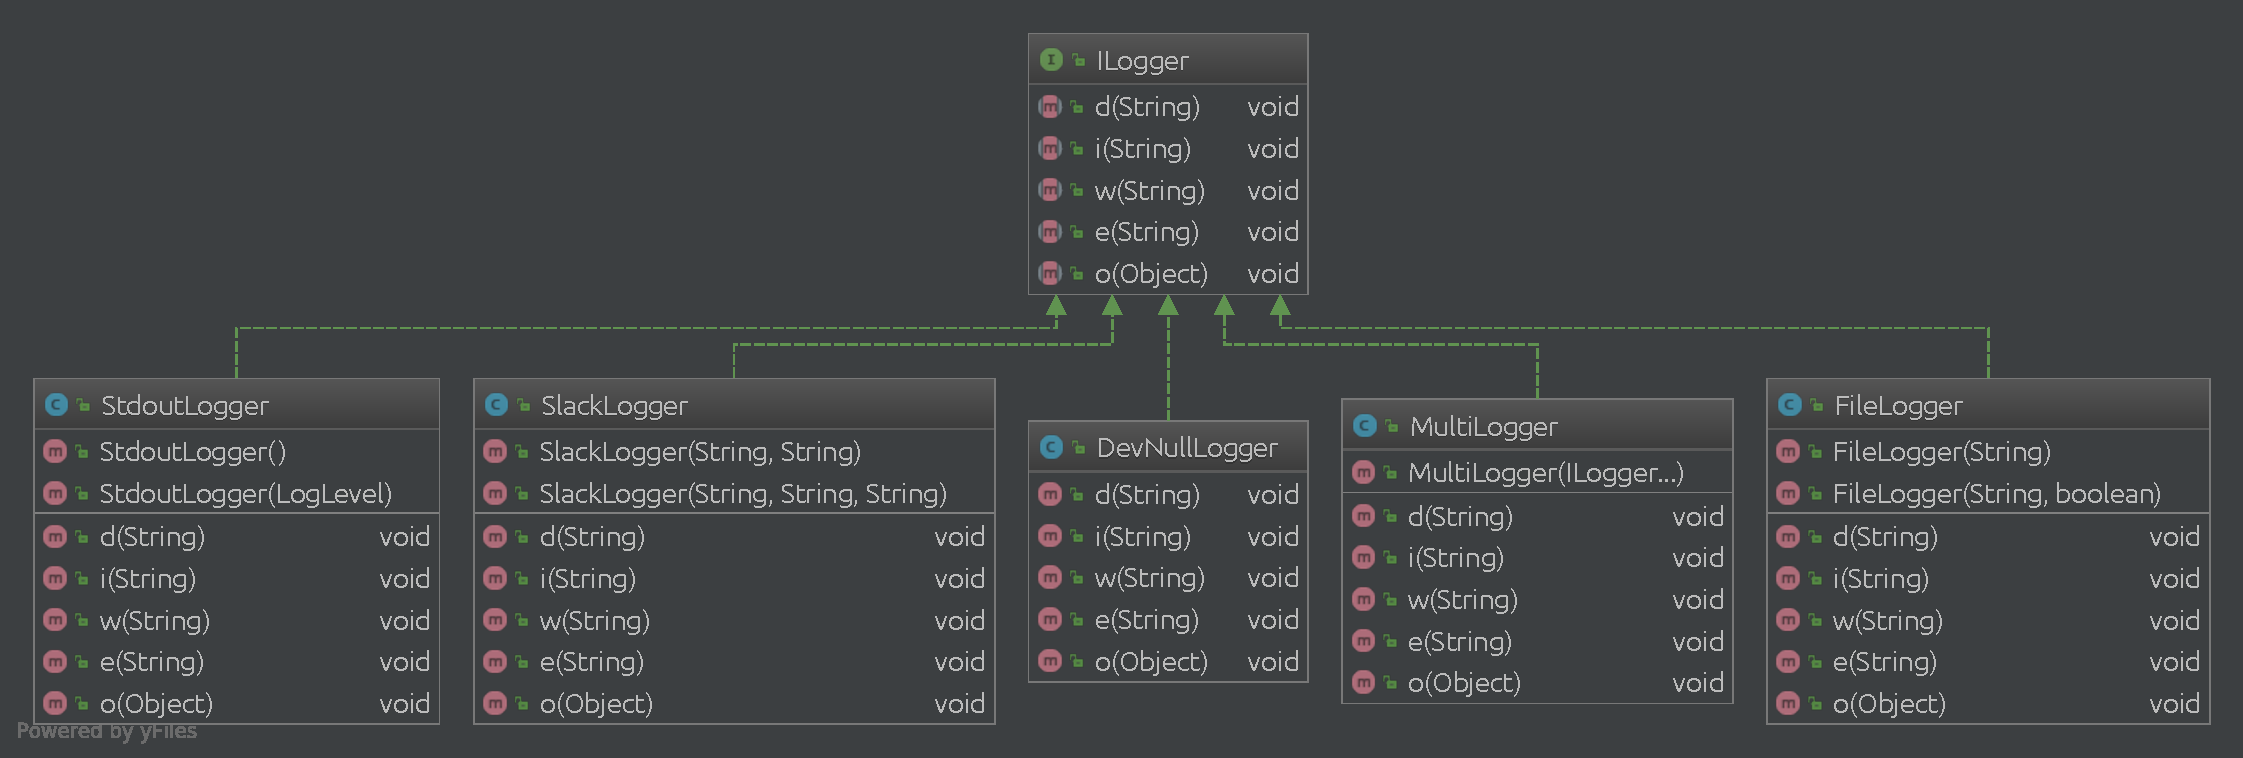
\includegraphics[width=\textwidth]{pkg_logs.pdf}
\centering
\caption{Paket $utils.logs$}
\label{fig:pkg_logs}
\end{figure}

Pri izvršavanju algoritma učenja ili pretrage predaje se objekt koji implementira sučelje $ILogger$. Objekt nudi metode za selektivno bilježenje informacija o izvođenju programa ili algoritma ovisno o njihovom tipu. Metode selektivnog bilježenja inspirirane su objektom $Log$ Java razvojne biblioteke operacijskog sustava Android. Postoji nekoliko izvedbi koje preusmjeravaju ulaze ostalim mehanizmima. Tablica \ref{tab:loggers} prikazuje implementacije i njihovo odredište.

\begin{table}[h]
\begin{tabular}{ll}
Klasa & Odredište \\
\hline
DevNullLogger & Ignorira ulaze \\
StdoutLogger & Standardni izlaz \\
FileLogger & Zapisuje u zadanu datoteku (s kreiranjem poddirektorija) \\
SlackLogger & Kanal servisa Slack \\
MultiLogger & Prosljeđuje listi zadanih implementacija
\end{tabular}
\centering
\caption{Implementacije za bilježenje}
\label{tab:loggers}
\end{table}

\subsection{Izvršni programi projekta}
U projektu su napisani brojni izvršni programi čije namjene uključuju demonstraciju dodataka, izvršavanje eksperimenata, ponavljanje eksperimenta s dodatnim bilježenjem i slično. U nastavku su opisani programi korišteni za izvršavanje eksperimenata.

\subsubsection{Pohlepna pretraga uobičajenih funkcija}
\todo{ulazi u program}
\todo{grid-search}

\subsubsection{Izgradnja aktivacijskih funkcija simboličkom regresijom}
\todo{ulazi u program}
\todo{procesni način rada}

%--------------------------------------------------------------------------------------%
\chapter{Rezultati}
\label{sec:rezultati}

\section{DPAv4}

\subsection{Usporedba uobičajenih aktivacijskih funkcija}

U ovom poglavlju prikazana je usporedba performansi popularnih aktivacijskih funkcija. Ispitivane su kombinacije arhitektura i aktivacijskih funkcija te su priložene postignute mjere točnosti i F1 mjere na skupu za testiranje. Za svaku kombinaciju arhitekture i aktivacijske funkcije provedeno je pretraživanje hiperparametara po rešetci i zabilježeni su najbolji postignuti rezultati. Zajednički i pretraživani hiperparametri navedeni su tablici \ref{tab:hp_common}. Najbolje kombinacije hiperparametara su navedene u dodatku \ref{app:grid_hp}.

\begin{table}
\centering
\begin{tabular}{lr}
Hiperparametar & Vrijednosti \\
\hline
Seed & 42 \\
Veličina minigrupe & 256 \\
Normalizacija značajki & Da \\
Permutacija mini-grupa & Ne \\
Normalizacija mini-grupe & Da \\
Dropout & Ne \\
Stopa opadanja stope učenja & 0.99 \\
Broj iteracija do idućeg opadanja stope učenja & 1 \\
Maksimalan broj epoha & 40 \\
Broj uzastopnih iteracija za rano zaustavljanje & 5 \\
Minimalna relativna promjena gubitka za detekciju konvergencije & 0.01 \\
\hline
Koeficijent L2 regularizacije & $10^{-3}$, $10^{-4}$, $10^{-5}$ \\
Stopa učenja & $10^{-3}$, $5 \cdot 10^{-4}$, $10^{-4}$
\end{tabular}
\caption{Hiperparametri korišteni pri učenju mreža. Zarezima su odvojene vrijednosti hiperparametara koje su pretraživane po rešetci.}
\label{tab:hp_common}
\end{table}

\begin{figure}[ht]
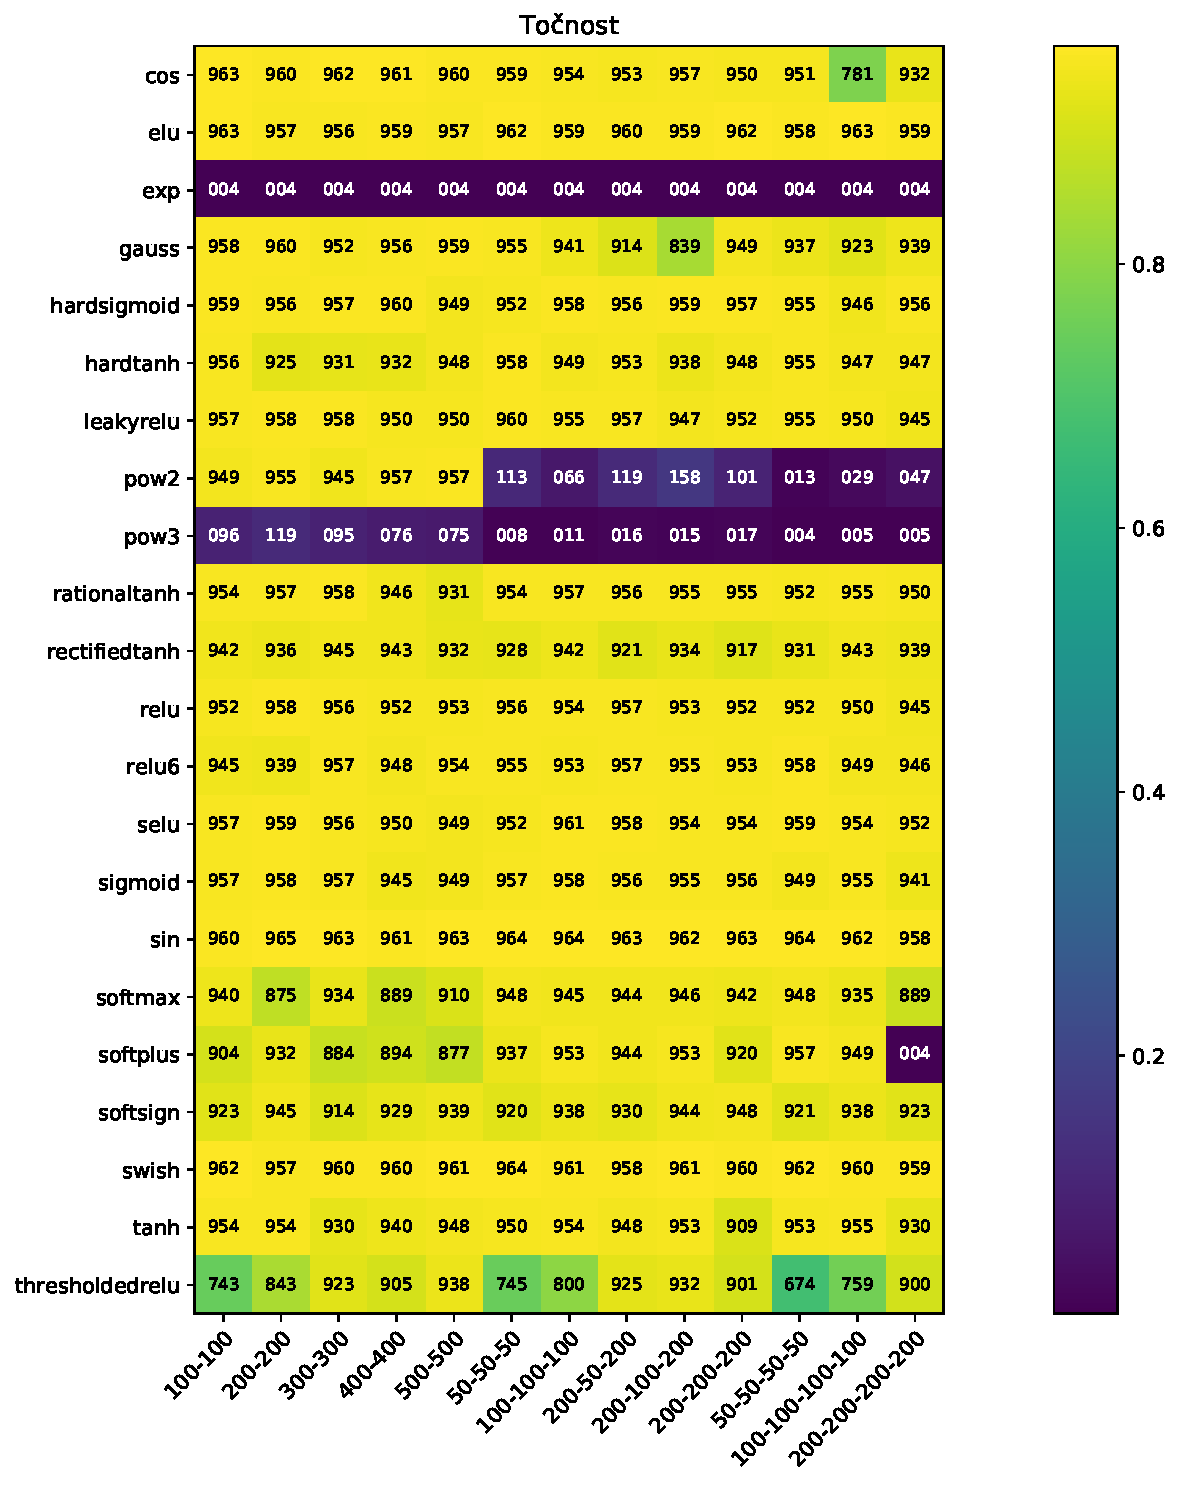
\includegraphics[width=\textwidth]{greedy_9_acc.pdf}
\centering
\caption{Postignuta točnost aktivacijskih funkcija na različitim arhitekturama. Vrijednosti u ćelijama su tri najznačajnije znamenke nakon točke. Na vrijednosti mjere $0.5$ tekst mijenja boju iz bijele u crnu.}
\label{fig:greedy_9_acc}
\end{figure}

\begin{figure}[ht]
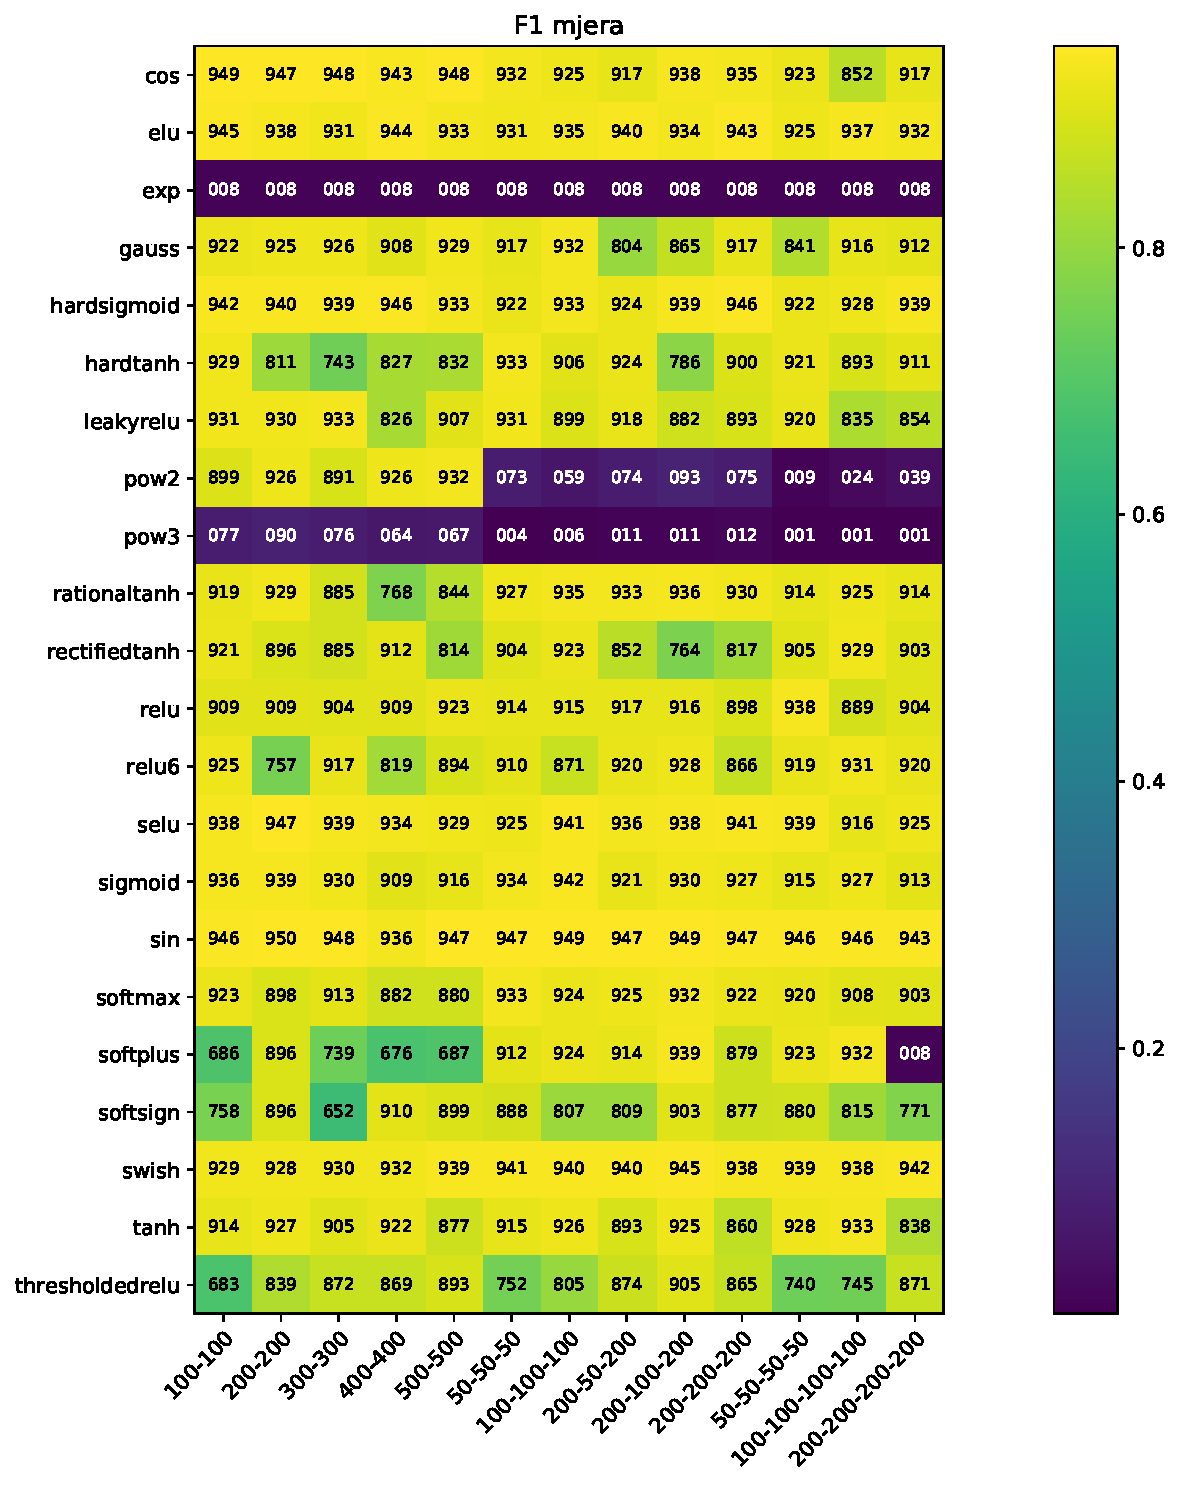
\includegraphics[width=\textwidth]{greedy_9_f1.pdf}
\centering
\caption{Postignuta F1 mjera aktivacijskih funkcija na različitim arhitekturama. Vrijednosti u ćelijama su tri najznačajnije znamenke nakon točke. Na vrijednosti mjere $0.5$ tekst mijenja boju iz bijele u crnu.}
\label{fig:greedy_9_f1}
\end{figure}

\begin{figure}[ht]
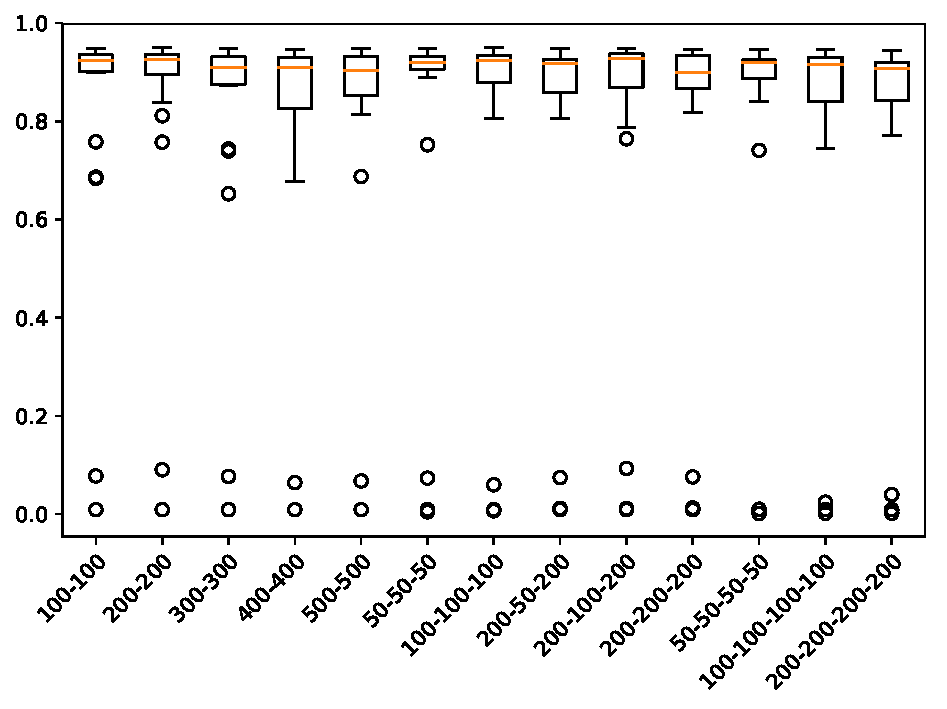
\includegraphics[width=.8\textwidth]{greedy_9_arch_quality.pdf}
\centering
\caption{Prosječna F1 mjera po svim arhitekturama. Ignorirani su rezultati funkcija kojima mreža nije uspješno naučena ($exp,pow2,pow3$). Najveću sumu ostvaruje arhitektura \textbf{[50-50-50]} te se upravo ona koristi za daljnjim eksperimentima. Koristi se najčešća kombinacija hiperparametara za tu arhitekturu je pod \textbf{indeksom 5} tablice \ref{tab:hp_comb}.}
\label{fig:greedy_9_arch_quality}
\end{figure}

\clearpage

\subsection{Izgradnja aktivacijskih funkcija simboličkom regresijom}
\todo{Tablica}
\todo{Komentar}
\todoimg{boxplot usporedba po taboo veličini}

\subsection{Izgradnja heterogenog rasporeda aktivacijskih funkcija}
\todo{Ne znam hoću li stići i ovo izvrtiti. Za najbolju prethodnu arhitekturu ću pronaći najbolji raspored uobičajenih fja po slojevima mreže (npr. sin-relu).}

\section{DPAv2}

\subsection{Usporedba uobičajenih aktivacijskih funkcija}

U ovom poglavlju prikazana je usporedba performansi popularnih aktivacijskih funkcija. Ispitivane su kombinacije arhitektura i aktivacijskih funkcija te su priložene postignute mjere točnosti i F1 mjere na skupu za testiranje. Za svaku kombinaciju arhitekture i aktivacijske funkcije provedeno je pretraživanje hiperparametara po rešetci i zabilježeni su najbolji postignuti rezultati. Zajednički i pretraživani hiperparametri identični su eksperimentima za DPAv2 (tablica \ref{tab:hp_common}). Najbolje kombinacije hiperparametara su navedene u dodatku \ref{app:grid_hp}.

\begin{figure}[ht]
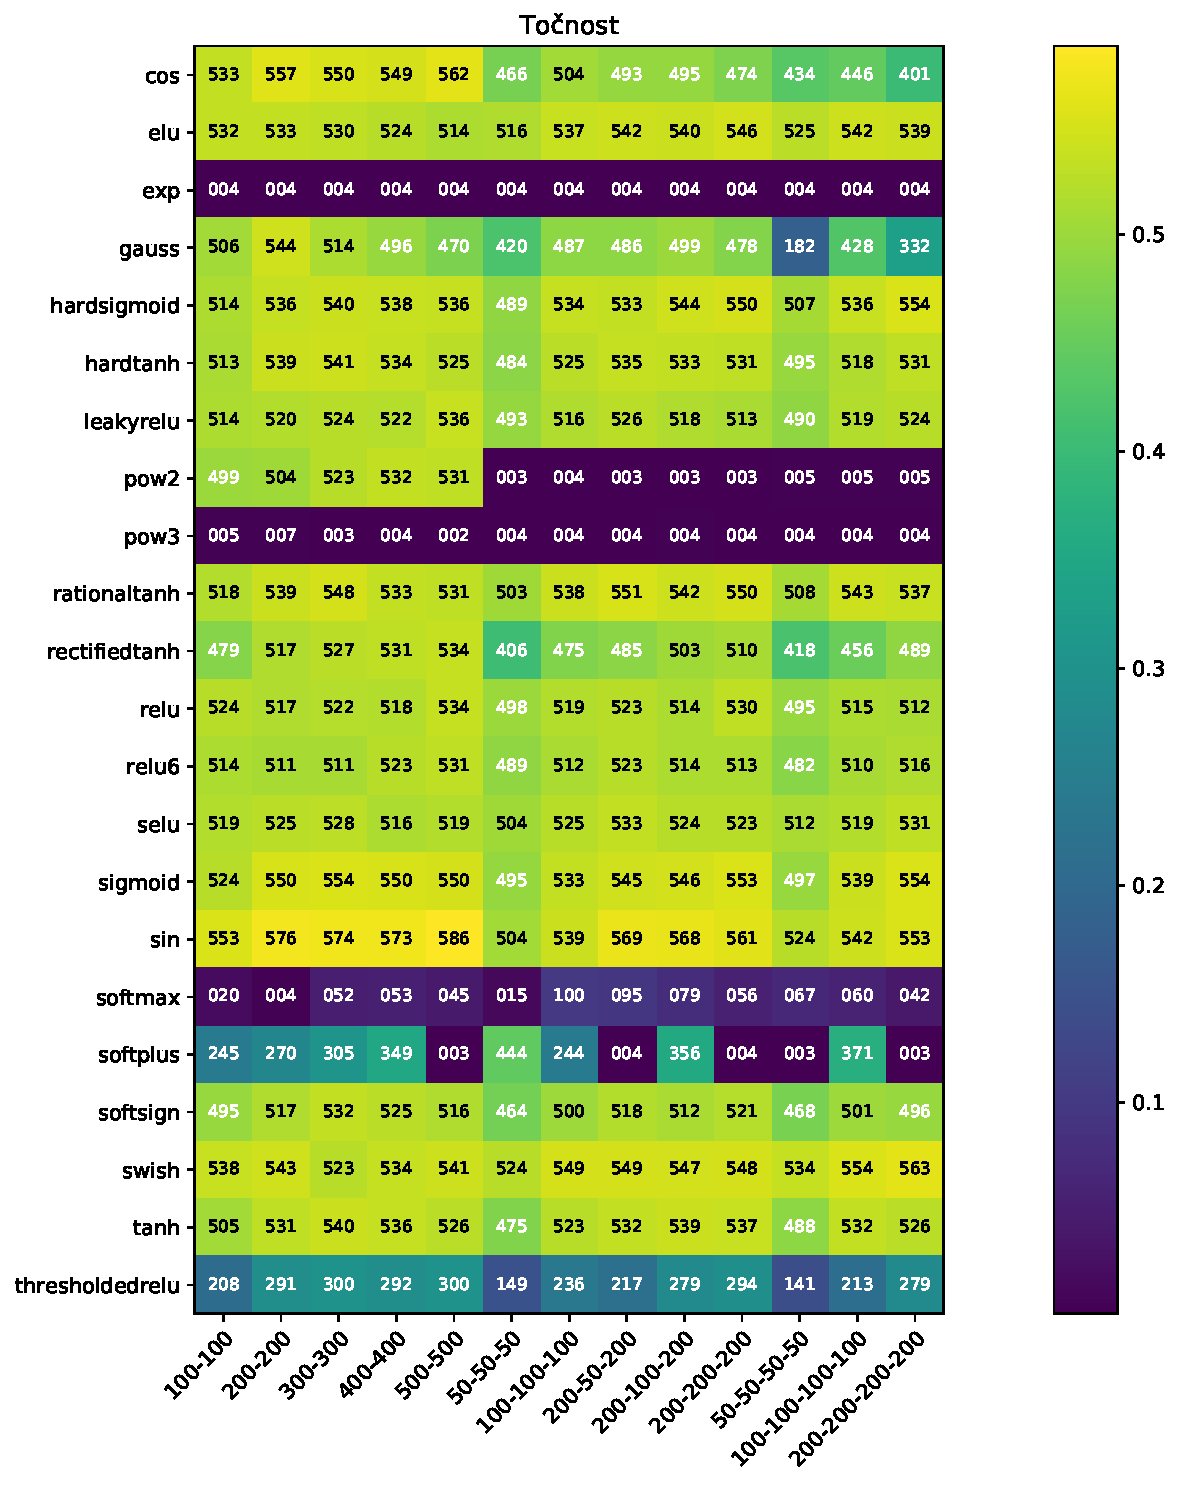
\includegraphics[width=\textwidth]{greedy_256_acc.pdf}
\centering
\caption{Postignuta točnost aktivacijskih funkcija na različitim arhitekturama. Vrijednosti u ćelijama su tri najznačajnije znamenke nakon točke. Na vrijednosti mjere $0.5$ tekst mijenja boju iz bijele u crnu.}
\label{fig:greedy_256_acc}
\end{figure}

\begin{figure}[ht]
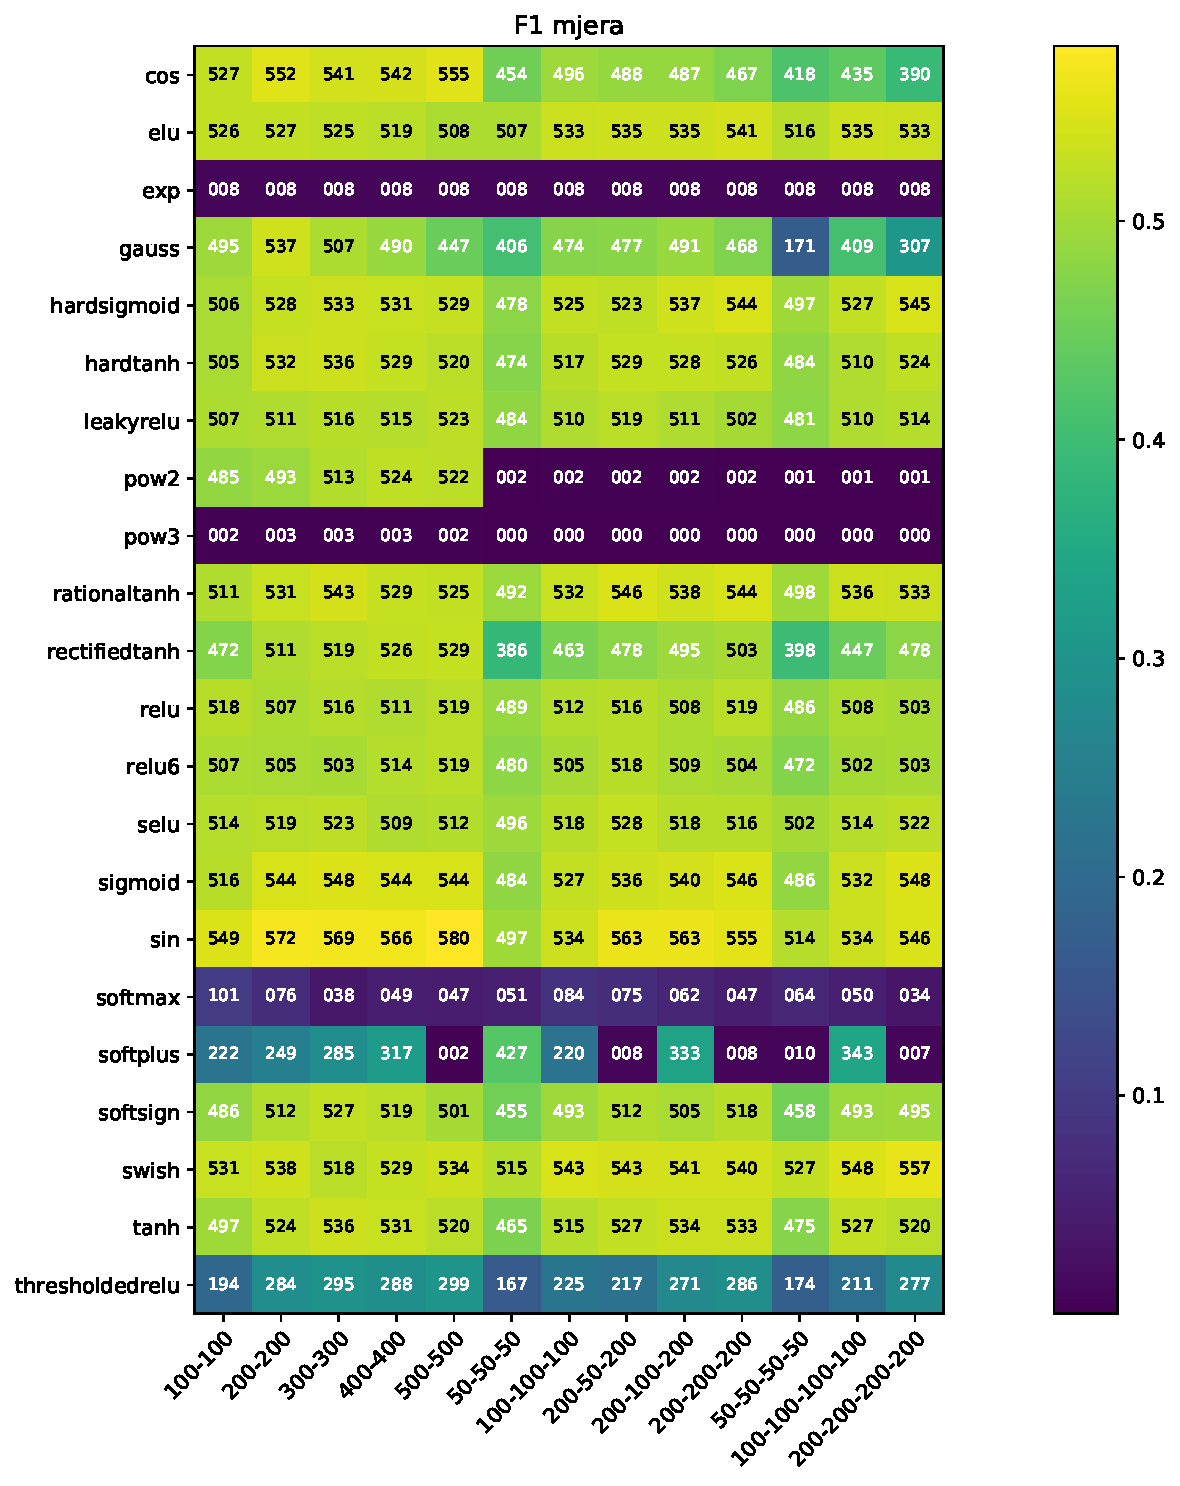
\includegraphics[width=\textwidth]{greedy_256_f1.pdf}
\centering
\caption{Postignuta F1 mjera aktivacijskih funkcija na različitim arhitekturama. Vrijednosti u ćelijama su tri najznačajnije znamenke nakon točke. Na vrijednosti mjere $0.5$ tekst mijenja boju iz bijele u crnu.}
\label{fig:greedy_256_f1}
\end{figure}

\clearpage

\todoimg{mjesta aktivacije top 4 funkcije po arh}
\todo{Komentar}

\todoimg{mjesta aktivacije bottom 4 funkcije po arh}
\todo{Komentar}

\todo{analiza slučaja pow2}

\begin{figure}[ht]
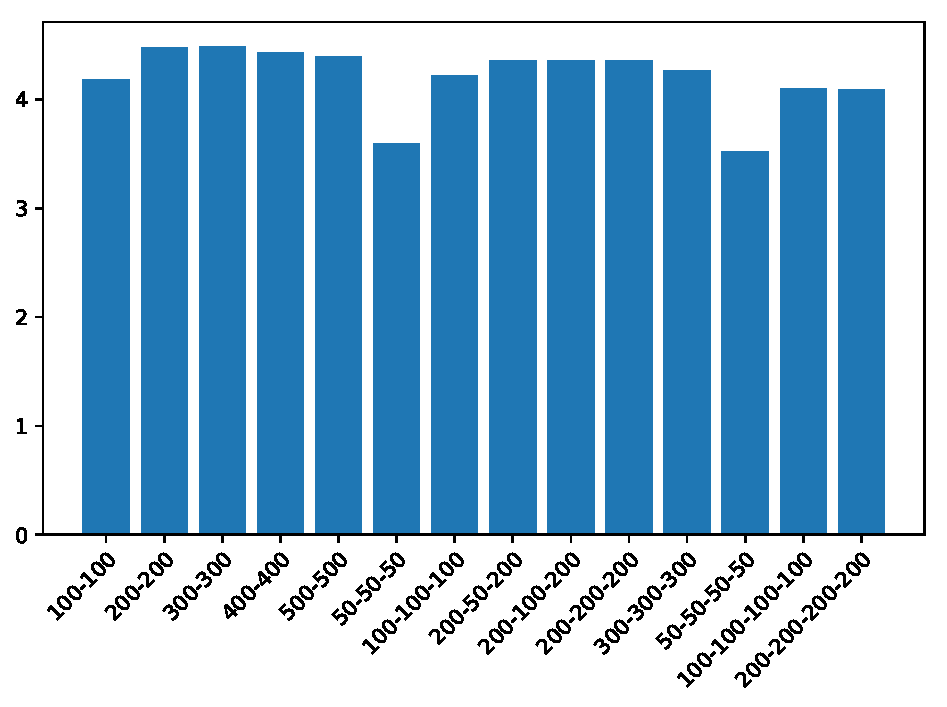
\includegraphics[width=.8\textwidth]{greedy_256_arch_quality.pdf}
\centering
\caption{Prosječna F1 mjera po svim arhitekturama. Ignorirani su rezultati funkcija kojima mreža nije uspješno naučena ($exp,pow2,pow3,softmax,softplus,thresholdedrelu$). Najveću sumu ostvaruje arhitektura \textbf{[300-300]} te se upravo ona koristi za daljnjim eksperimentima. Koristi se najčešća kombinacija hiperparametara za tu arhitekturu je pod \textbf{indeksom 5} tablice \ref{tab:hp_256_comb}.}
\label{fig:greedy_256_arch_quality}
\end{figure}

\clearpage

\subsection{Izgradnja aktivacijskih funkcija simboličkom regresijom}

\todo{Tablica}
\todo{Komentar}
\todoimg{boxplot usporedba po taboo veličini}

\subsection{Izgradnja heterogenog rasporeda aktivacijskih funkcija}
\todo{Ne znam hoću li stići i ovo izvrtiti. Za najbolju prethodnu arhitekturu ću pronaći najbolji raspored uobičajenih fja po slojevima mreže (npr. sin-relu).}

%--------------------------------------------------------------------------------------%
\chapter{Stvari koje sam probao, ali nisu ispale korisne}
\subsubsection{Učeći parametri}
\todo{dokaz da na korištene funkcije nema utjecaja (stopi se s težinama ili biasom)}
\todo{pokazati primjer fje gdje bi se mogao koristiti}

\subsubsection{Dropout}
Dropout \citep{dropout} je tehnika regularizacije neuronskih mreža koja ostvaruje dobre rezultate na vrlo dubokim i širokim modelima koji su skloni pretreniranju i koadaptaciji neurona. Radi tako da za vrijeme učenja mreže proporcionalno zadanoj vjerojatnosti nasumično isključuje neurone u oba smjera. Tehnika efikasno sprječava koadaptaciju neurona širokih slojeva jer je vjerojatnost da će dva neurona koji su skloni koadaptaciji biti identično naučena vrlo mala. Isključivani neuroni će ipak učiti jer vjerojatnost da će neuron ostati isključen kroz više iteracija obrnuto proporcionalna broju iteracija.

Negativna posljedica Dropout-a je dulje vrijeme učenja jer je potrebno više iteracija da svaki neuron dobije dovoljan broj efektivnih iteracija učenja. Ta činjenica nije korisna za postupke neuroevolucije kojima trošak evaluacije definira traktabilnost postupka. U sklopu projekta, provedeni su i preliminarni eksperimenti koji su dokazali spomenutu neučinkovitost.

\subsubsection{Tensorflow Java API}
\todo{probo, ali je još u razvoju (puno toga je falilo)}

%--------------------------------------------------------------------------------------%
\chapter{Buduća istraživanja}
\todo{Primjena CNN na sirovim vremenskim uzorcima po uzoru na onaj rad}
\todo{Ispitivanje učinkovitosti korištene optimizacije na ostalim zadatcima}
\todo{Operatori različitog utjecaja i uzorkovanje s rastućim pragom osjetljivosti na izmjene populacije. Operatori imaju definiranu snagu, kako vrijeme ide sve manje se biraju (putujuća sigmoida) snažni operatori -> konvergencija kao sim. kaljenje}
\todo{Paralelna evolucija arhitekture i aktivacijskih fja \citep{cnn_evolution}}

%--------------------------------------------------------------------------------------%
\chapter{Zaključak}
\todo{Radi/Ne radi}
\todo{Pronađene zanimljivosti}
\todo{Pouka za doma}

\bibliography{literatura}
\bibliographystyle{fer}

\begin{sazetak}
Proučiti postojeće metode u izgradnji aktivacijskih funkcija u umjetnim neuronskim mrežama. Posebnu pažnju posvetiti evolucijskim algoritmima simboličke regresije za izgradnju ciljanih funkcija. Ustanoviti moguće nedostatke postojećih algoritama ili mogućnost poboljšanja. Primijeniti evoluirane aktivacijske funkcije u homogenoj ili heterogenoj umjetnoj neuronskoj mreži na skupovima DPAv2 i DPAv4 te odrediti mjere kvalitete izgrađenog klasifikatora: točnost, preciznost, odziv te F mjere. Usporediti učinkovitost ostvarenih postupaka s postojećim rješenjima iz literature. Radu priložiti izvorne tekstove programa, dobivene rezultate uz potrebna objašnjenja i korištenu literaturu.

\kljucnerijeci{Ključne riječi, odvojene zarezima.}
\end{sazetak}

\engtitle{Optimized activation functions for classifiers based on artificial neural networks in the domain of implementation attacks on cryptographic devices}
\begin{abstract}
Examine existing methods in building activation functions in artificial neural networks. Give special attention to evolutionary algorithms of symbolic regression for constructing the targeted functions. Apply evolved activation functions in a homogeneous or heterogeneous artificial neural network on datasets DPAv2 and DPAv4 and examine quality measures of the built classifier: accuracy, precision, recall and F measures. Compare the efficiency of acquired methods with existing solutions from the literature. Alongside thesis attach source code of programs, acquired results with necessarry discussion and literature used.

\keywords{Keywords.}
\end{abstract}

\appendix
\chapter{Hiperparametri pretrage po rešetci}
\label{app:grid_hp}

\begin{table}
\centering
\begin{tabular}{lcc}
Indeks & Koeficijent L2 reg. & Stopa učenja \\
\hline
1 & $10^{-3}$ & $10^{-3}$  \\
2 & $10^{-3}$ & $5 \cdot 10^{-4}$ \\
3 & $10^{-3}$ & $10^{-4}$ \\
4 & $10^{-4}$ & $10^{-3}$ \\
5 & $10^{-4}$ & $5 \cdot 10^{-4}$ \\
6 & $10^{-4}$ & $10^{-4}$ \\
7 & $10^{-5}$ & $10^{-3}$ \\
8 & $10^{-5}$ & $5 \cdot 10^{-4}$ \\
9 & $10^{-5}$ & $10^{-4}$
\end{tabular}
\caption{Indeksi kombinacija hiperparametara korištenih pri pretraživanju po rešetci.}
\label{tab:hp_comb}
\end{table}

\begin{figure}[ht]
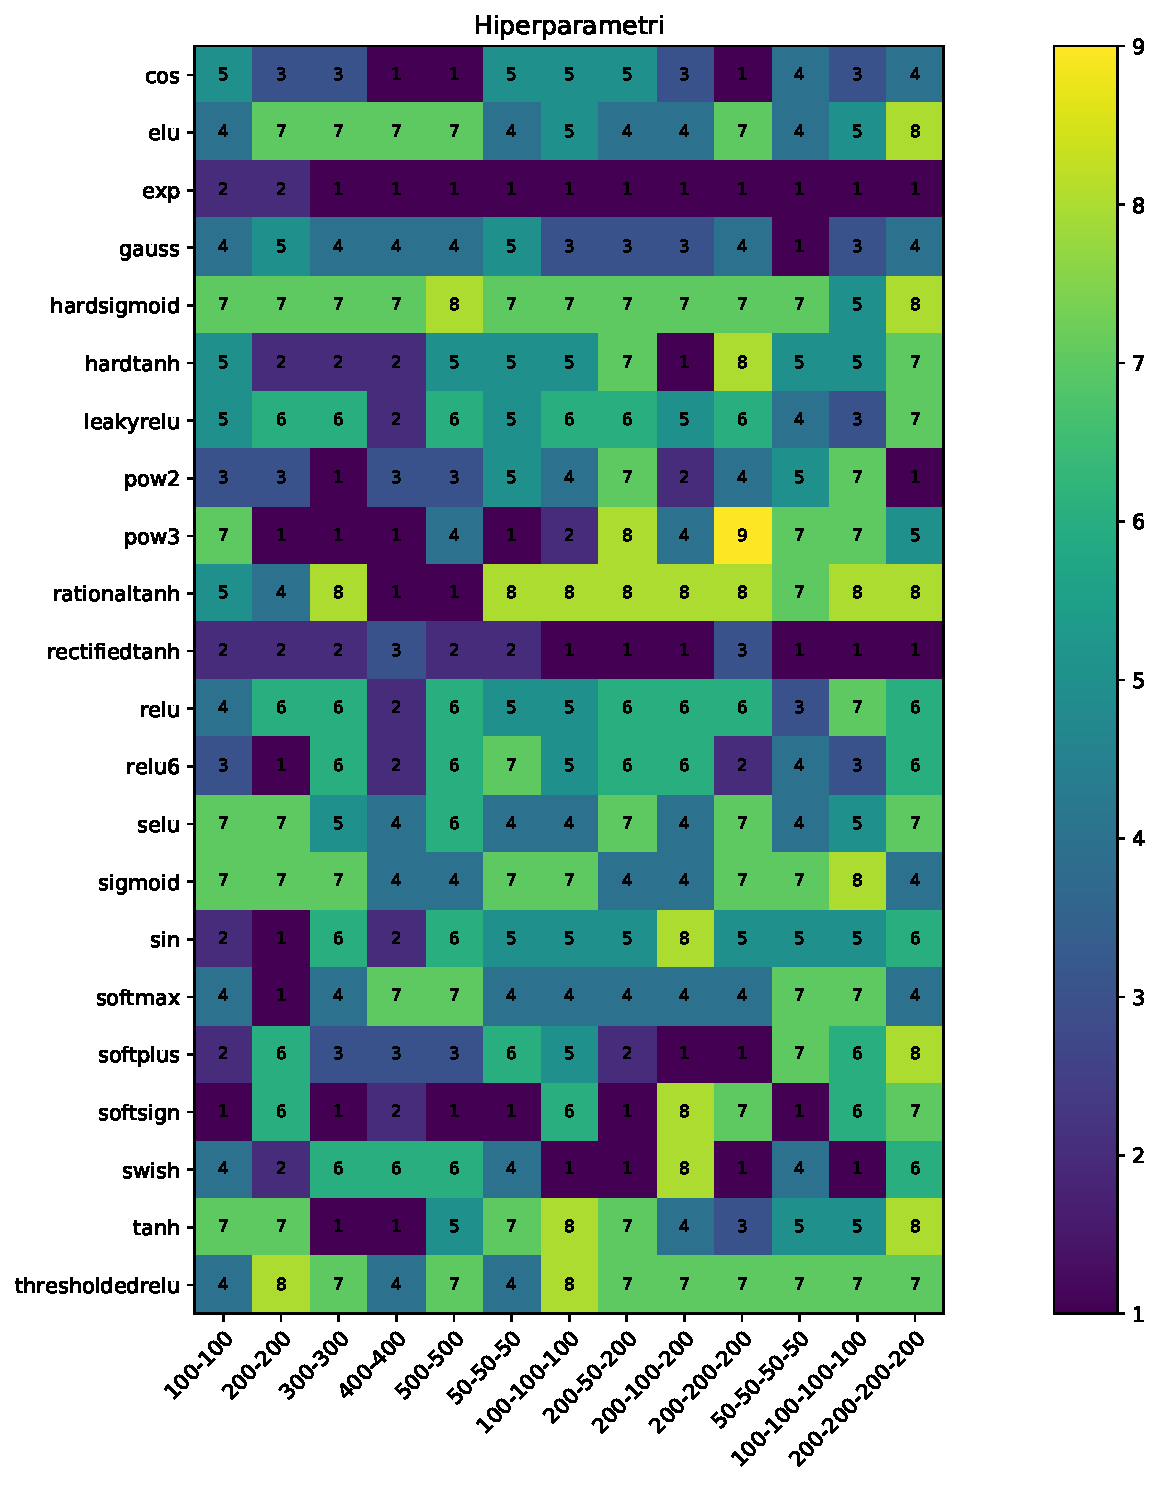
\includegraphics[width=\textwidth]{greedy_9_hp.pdf}
\centering
\caption{Skup \textbf{DPAv4}: Optimalne kombinacije hiperparametara za aktivacijske funkcije na različitim arhitekturama. Vrijednosti u ćelijama označavaju kombinacije hiperparametara navedene u tablici \ref{tab:hp_comb}}
\label{fig:greedy_9_hp}
\end{figure}

\begin{figure}[ht]
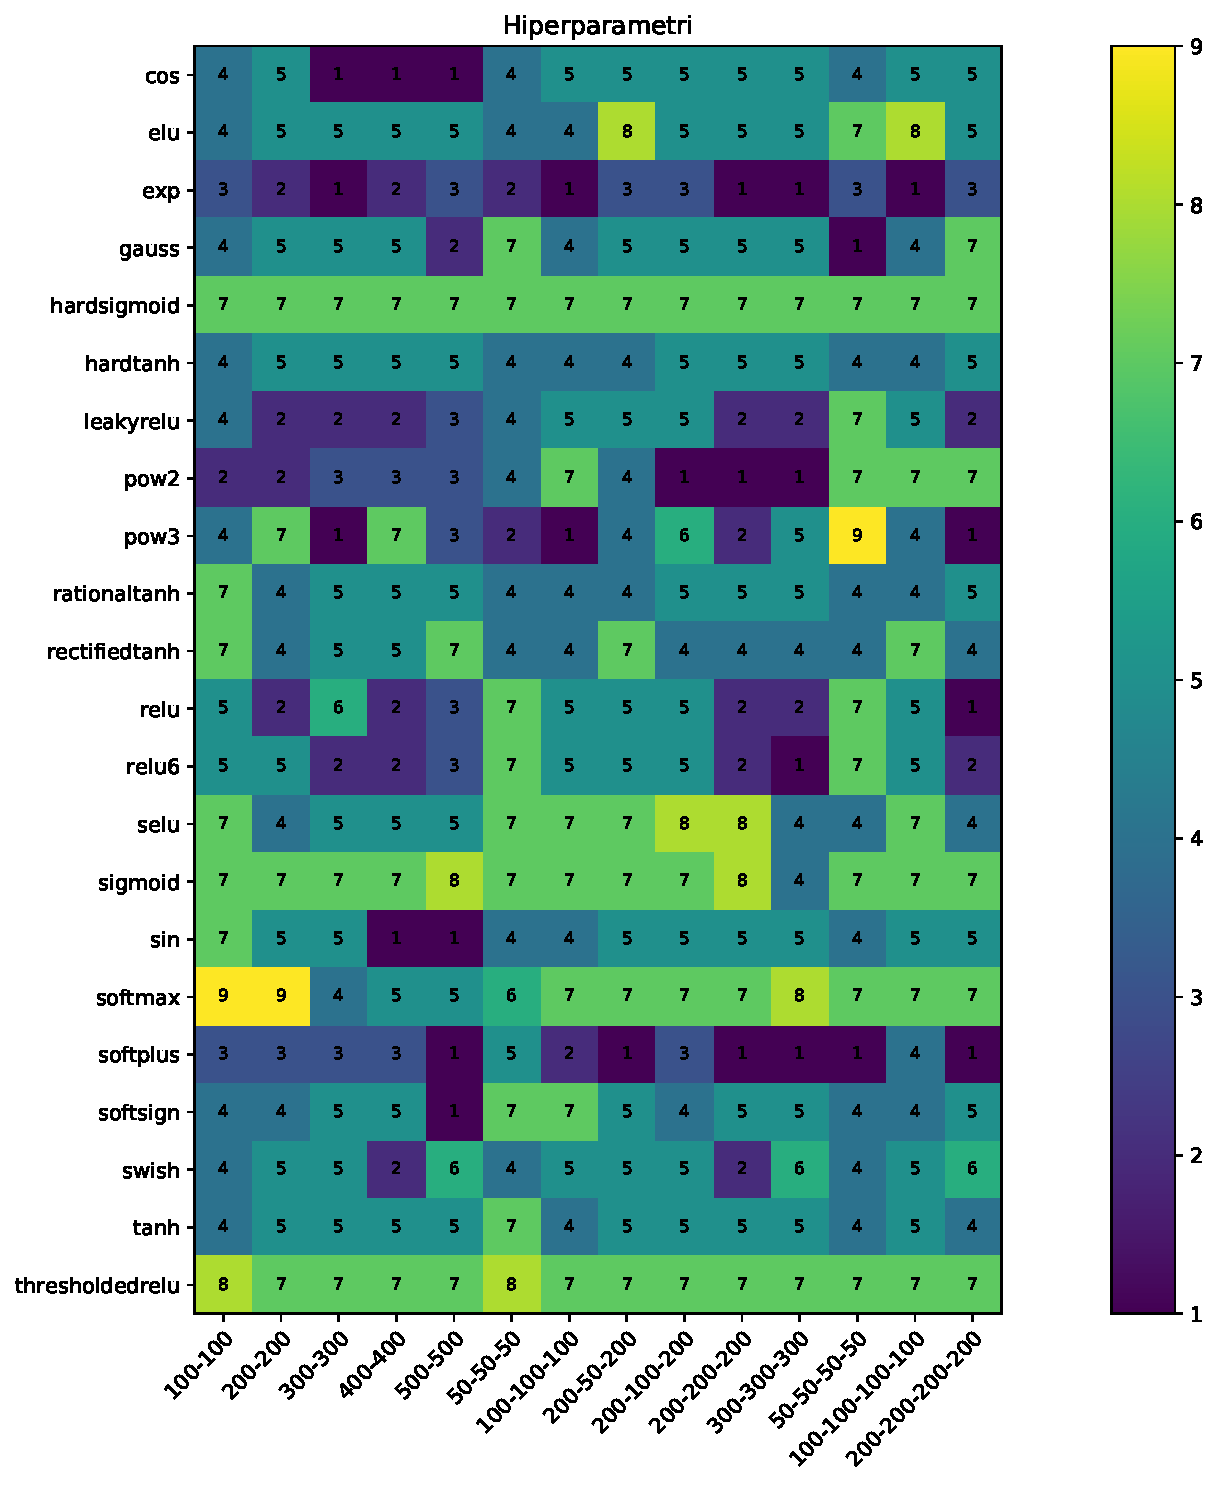
\includegraphics[width=\textwidth]{greedy_256_hp.pdf}
\centering
\caption{Skup \textbf{DPAv2}: Optimalne kombinacije hiperparametara za aktivacijske funkcije na različitim arhitekturama. Vrijednosti u ćelijama označavaju kombinacije hiperparametara navedene u tablici \ref{tab:hp_comb}}
\label{fig:greedy_256_hp}
\end{figure}

\end{document}
